\bigskip

\bigskip

Dla prostoty i przejrzystości sprawozdania wykorzystane zostały oznaczenia pierwotnie wprowadzone w skrypcie z przedmiotu STP.

\bigskip

Zadane wartości:

\smallskip

W1=W2=50\%

\smallskip

$\mathrm{G1_{pp}}=30$

\smallskip

$\mathrm{G2_{pp}}=35$

\smallskip

$T=4s$ (okres próbkowania)

\bigskip

Ograniczenia:

\smallskip

$0 \le \mathrm{G1}(k) \le 100$

$0 \le \mathrm{G2}(k) \le 100$

\chapter{Podpunkt 1}
Sprawdzenie możliwości sterowania i pomiaru w komunikacji ze stanowiskiem odbyło się po wgraniu początkowego kodu poprzez wysłanie do stanowiska kilku różnych wartości sterowania i zaobserwowanie odpowiedniej odpowiedzi stanowiska oraz zmian w napływających danych.

Pomiar wartości temperatur w punkcie pracy odbył się zgodnie z poleceniem poprzez zadanie wartości sygnałów W1, W2 oraz G1, G2, a następnie zarejestrowanie wartości sygnałów T1, T3 po ustabilizowaniu się układu. Otrzymane wartości to $\mathrm{T1_{pp}}=\num{36,5}$ oraz $\mathrm{T3_{pp}}=\num{38,3}$.

\begin{figure}[ht]
\centering
% This file was created by matlab2tikz.
%
%The latest updates can be retrieved from
%  http://www.mathworks.com/matlabcentral/fileexchange/22022-matlab2tikz-matlab2tikz
%where you can also make suggestions and rate matlab2tikz.
%
\definecolor{mycolor1}{rgb}{0.00000,0.44700,0.74100}%
%
\begin{tikzpicture}

\begin{axis}[%
width=4.521in,
height=3.566in,
at={(0.758in,0.481in)},
scale only axis,
xmin=0,
xmax=350,
xtick={0,50,100,150,200,250,300,350},
xlabel style={font=\color{white!15!black}},
xlabel={k},
ymin=27,
ymax=36,
ytick={27,28,29,30,31,32,33,34,35,36},
ylabel style={font=\color{white!15!black}},
ylabel={T1},
axis background/.style={fill=white}
]
\addplot [color=mycolor1, forget plot]
  table[row sep=crcr]{%
1	27.25\\
2	27.25\\
3	27.25\\
4	27.25\\
5	27.25\\
6	27.31\\
7	27.31\\
8	27.31\\
9	27.37\\
10	27.43\\
11	27.43\\
12	27.5\\
13	27.5\\
14	27.56\\
15	27.62\\
16	27.62\\
17	27.68\\
18	27.75\\
19	27.81\\
20	27.87\\
21	27.93\\
22	28\\
23	28.06\\
24	28.12\\
25	28.18\\
26	28.25\\
27	28.31\\
28	28.37\\
29	28.43\\
30	28.5\\
31	28.56\\
32	28.62\\
33	28.75\\
34	28.75\\
35	28.87\\
36	28.93\\
37	29\\
38	29.06\\
39	29.12\\
40	29.25\\
41	29.31\\
42	29.31\\
43	29.43\\
44	29.5\\
45	29.56\\
46	29.62\\
47	29.68\\
48	29.75\\
49	29.81\\
50	29.87\\
51	29.93\\
52	30.06\\
53	30.12\\
54	30.18\\
55	30.25\\
56	30.31\\
57	30.43\\
58	30.5\\
59	30.56\\
60	30.68\\
61	30.75\\
62	30.81\\
63	30.87\\
64	30.93\\
65	31\\
66	31.06\\
67	31.12\\
68	31.18\\
69	31.25\\
70	31.25\\
71	31.31\\
72	31.37\\
73	31.43\\
74	31.5\\
75	31.5\\
76	31.56\\
77	31.62\\
78	31.68\\
79	31.68\\
80	31.75\\
81	31.81\\
82	31.87\\
83	31.93\\
84	31.93\\
85	32\\
86	32.06\\
87	32.06\\
88	32.12\\
89	32.18\\
90	32.18\\
91	32.25\\
92	32.31\\
93	32.31\\
94	32.37\\
95	32.37\\
96	32.43\\
97	32.5\\
98	32.5\\
99	32.56\\
100	32.62\\
101	32.62\\
102	32.68\\
103	32.75\\
104	32.75\\
105	32.75\\
106	32.81\\
107	32.87\\
108	32.87\\
109	32.87\\
110	32.93\\
111	33\\
112	33\\
113	33.06\\
114	33.12\\
115	33.12\\
116	33.12\\
117	33.18\\
118	33.18\\
119	33.25\\
120	33.25\\
121	33.31\\
122	33.31\\
123	33.31\\
124	33.37\\
125	33.37\\
126	33.43\\
127	33.43\\
128	33.43\\
129	33.5\\
130	33.5\\
131	33.56\\
132	33.56\\
133	33.56\\
134	33.62\\
135	33.62\\
136	33.62\\
137	33.62\\
138	33.68\\
139	33.68\\
140	33.68\\
141	33.75\\
142	33.75\\
143	33.81\\
144	33.81\\
145	33.87\\
146	33.87\\
147	33.93\\
148	33.87\\
149	33.93\\
150	34\\
151	34\\
152	34\\
153	34\\
154	34.06\\
155	34.06\\
156	34.06\\
157	34.12\\
158	34.12\\
159	34.12\\
160	34.18\\
161	34.18\\
162	34.18\\
163	34.25\\
164	34.25\\
165	34.25\\
166	34.31\\
167	34.31\\
168	34.31\\
169	34.31\\
170	34.37\\
171	34.37\\
172	34.37\\
173	34.37\\
174	34.37\\
175	34.43\\
176	34.43\\
177	34.43\\
178	34.5\\
179	34.43\\
180	34.5\\
181	34.5\\
182	34.5\\
183	34.5\\
184	34.56\\
185	34.56\\
186	34.56\\
187	34.56\\
188	34.56\\
189	34.56\\
190	34.62\\
191	34.62\\
192	34.62\\
193	34.62\\
194	34.62\\
195	34.62\\
196	34.68\\
197	34.68\\
198	34.68\\
199	34.68\\
200	34.68\\
201	34.68\\
202	34.68\\
203	34.68\\
204	34.68\\
205	34.68\\
206	34.68\\
207	34.68\\
208	34.68\\
209	34.68\\
210	34.75\\
211	34.75\\
212	34.75\\
213	34.75\\
214	34.75\\
215	34.81\\
216	34.81\\
217	34.81\\
218	34.81\\
219	34.81\\
220	34.81\\
221	34.81\\
222	34.87\\
223	34.87\\
224	34.87\\
225	34.87\\
226	34.87\\
227	34.87\\
228	34.87\\
229	34.87\\
230	34.93\\
231	34.93\\
232	34.93\\
233	34.93\\
234	34.93\\
235	34.93\\
236	34.93\\
237	34.93\\
238	34.93\\
239	34.93\\
240	34.93\\
241	34.93\\
242	34.93\\
243	34.93\\
244	35\\
245	35\\
246	35\\
247	35\\
248	35\\
249	35\\
250	35\\
251	35\\
252	35\\
253	35.06\\
254	35.06\\
255	35.06\\
256	35.06\\
257	35.06\\
258	35.06\\
259	35.06\\
260	35.06\\
261	35.06\\
262	35.06\\
263	35.06\\
264	35.06\\
265	35.06\\
266	35.12\\
267	35.06\\
268	35.12\\
269	35.12\\
270	35.06\\
271	35.06\\
272	35.12\\
273	35.12\\
274	35.12\\
275	35.12\\
276	35.12\\
277	35.12\\
278	35.12\\
279	35.12\\
280	35.12\\
281	35.12\\
282	35.12\\
283	35.12\\
284	35.12\\
285	35.12\\
286	35.12\\
287	35.12\\
288	35.12\\
289	35.12\\
290	35.12\\
291	35.12\\
292	35.12\\
293	35.12\\
294	35.12\\
295	35.12\\
296	35.12\\
297	35.12\\
298	35.12\\
299	35.12\\
300	35.12\\
301	35.12\\
302	35.12\\
303	35.12\\
304	35.12\\
305	35.12\\
306	35.12\\
307	35.18\\
308	35.18\\
309	35.18\\
310	35.18\\
311	35.18\\
312	35.12\\
313	35.12\\
314	35.12\\
315	35.12\\
316	35.12\\
317	35.12\\
318	35.18\\
319	35.12\\
320	35.18\\
321	35.18\\
322	35.12\\
323	35.18\\
324	35.18\\
325	35.18\\
326	35.18\\
327	35.18\\
328	35.18\\
329	35.25\\
330	35.25\\
331	35.25\\
332	35.25\\
333	35.25\\
334	35.25\\
335	35.25\\
336	35.25\\
337	35.25\\
338	35.25\\
339	35.25\\
340	35.25\\
341	35.31\\
342	35.31\\
343	35.31\\
344	35.31\\
345	35.31\\
346	35.31\\
347	35.31\\
348	35.31\\
349	35.31\\
350	35.31\\
};
\end{axis}
\end{tikzpicture}%
\caption{Pomiar T1 w punkcie pracy}
\label{Z1T1}
\end{figure}

\begin{figure}[ht]
\centering
% This file was created by matlab2tikz.
%
%The latest updates can be retrieved from
%  http://www.mathworks.com/matlabcentral/fileexchange/22022-matlab2tikz-matlab2tikz
%where you can also make suggestions and rate matlab2tikz.
%
\definecolor{mycolor1}{rgb}{0.00000,0.44700,0.74100}%
%
\begin{tikzpicture}

\begin{axis}[%
width=4.521in,
height=3.566in,
at={(0.758in,0.481in)},
scale only axis,
xmin=0,
xmax=350,
xtick={0,50,100,150,200,250,300,350},
xlabel style={font=\color{white!15!black}},
xlabel={$k$},
ymin=27,
ymax=36,
ytick={27,28,29,30,31,32,33,34,35,36},
ylabel style={font=\color{white!15!black}},
ylabel={T3},
axis background/.style={fill=white}
]
\addplot [color=mycolor1, forget plot]
  table[row sep=crcr]{%
1	27.5\\
2	27.5\\
3	27.43\\
4	27.43\\
5	27.5\\
6	27.5\\
7	27.5\\
8	27.5\\
9	27.5\\
10	27.5\\
11	27.56\\
12	27.62\\
13	27.62\\
14	27.68\\
15	27.68\\
16	27.75\\
17	27.81\\
18	27.81\\
19	27.93\\
20	27.93\\
21	28\\
22	28.06\\
23	28.12\\
24	28.18\\
25	28.25\\
26	28.31\\
27	28.37\\
28	28.43\\
29	28.5\\
30	28.62\\
31	28.68\\
32	28.75\\
33	28.81\\
34	28.87\\
35	28.93\\
36	29.06\\
37	29.12\\
38	29.18\\
39	29.25\\
40	29.37\\
41	29.43\\
42	29.5\\
43	29.56\\
44	29.68\\
45	29.75\\
46	29.81\\
47	29.87\\
48	30\\
49	30.06\\
50	30.12\\
51	30.18\\
52	30.25\\
53	30.31\\
54	30.43\\
55	30.43\\
56	30.56\\
57	30.62\\
58	30.68\\
59	30.75\\
60	30.81\\
61	30.87\\
62	30.93\\
63	31\\
64	31.06\\
65	31.12\\
66	31.18\\
67	31.25\\
68	31.31\\
69	31.37\\
70	31.43\\
71	31.5\\
72	31.56\\
73	31.62\\
74	31.68\\
75	31.68\\
76	31.75\\
77	31.81\\
78	31.87\\
79	31.93\\
80	31.93\\
81	32\\
82	32.06\\
83	32.12\\
84	32.18\\
85	32.18\\
86	32.25\\
87	32.31\\
88	32.37\\
89	32.37\\
90	32.43\\
91	32.5\\
92	32.56\\
93	32.56\\
94	32.62\\
95	32.68\\
96	32.75\\
97	32.81\\
98	32.87\\
99	32.87\\
100	32.93\\
101	33\\
102	33\\
103	33.06\\
104	33.06\\
105	33.12\\
106	33.18\\
107	33.18\\
108	33.18\\
109	33.25\\
110	33.25\\
111	33.31\\
112	33.31\\
113	33.37\\
114	33.37\\
115	33.43\\
116	33.43\\
117	33.5\\
118	33.5\\
119	33.56\\
120	33.56\\
121	33.62\\
122	33.62\\
123	33.68\\
124	33.68\\
125	33.68\\
126	33.75\\
127	33.75\\
128	33.81\\
129	33.81\\
130	33.81\\
131	33.87\\
132	33.93\\
133	33.93\\
134	33.93\\
135	34\\
136	34.06\\
137	34.06\\
138	34.06\\
139	34.12\\
140	34.12\\
141	34.12\\
142	34.18\\
143	34.18\\
144	34.25\\
145	34.25\\
146	34.25\\
147	34.31\\
148	34.31\\
149	34.31\\
150	34.37\\
151	34.37\\
152	34.43\\
153	34.43\\
154	34.43\\
155	34.5\\
156	34.5\\
157	34.5\\
158	34.56\\
159	34.56\\
160	34.56\\
161	34.56\\
162	34.62\\
163	34.62\\
164	34.68\\
165	34.62\\
166	34.68\\
167	34.68\\
168	34.75\\
169	34.75\\
170	34.75\\
171	34.75\\
172	34.75\\
173	34.75\\
174	34.81\\
175	34.81\\
176	34.81\\
177	34.81\\
178	34.81\\
179	34.87\\
180	34.87\\
181	34.87\\
182	34.87\\
183	34.87\\
184	34.93\\
185	34.93\\
186	34.93\\
187	34.93\\
188	34.93\\
189	35\\
190	34.93\\
191	35\\
192	35\\
193	35\\
194	35\\
195	35\\
196	35.06\\
197	35.06\\
198	35.06\\
199	35.06\\
200	35.06\\
201	35.12\\
202	35.12\\
203	35.12\\
204	35.12\\
205	35.12\\
206	35.12\\
207	35.12\\
208	35.12\\
209	35.12\\
210	35.12\\
211	35.18\\
212	35.18\\
213	35.18\\
214	35.18\\
215	35.18\\
216	35.18\\
217	35.18\\
218	35.25\\
219	35.25\\
220	35.25\\
221	35.25\\
222	35.25\\
223	35.25\\
224	35.25\\
225	35.25\\
226	35.31\\
227	35.31\\
228	35.31\\
229	35.31\\
230	35.37\\
231	35.37\\
232	35.37\\
233	35.37\\
234	35.43\\
235	35.37\\
236	35.43\\
237	35.43\\
238	35.43\\
239	35.43\\
240	35.5\\
241	35.5\\
242	35.5\\
243	35.5\\
244	35.5\\
245	35.5\\
246	35.5\\
247	35.5\\
248	35.5\\
249	35.5\\
250	35.5\\
251	35.5\\
252	35.5\\
253	35.5\\
254	35.5\\
255	35.5\\
256	35.56\\
257	35.56\\
258	35.5\\
259	35.56\\
260	35.56\\
261	35.56\\
262	35.56\\
263	35.56\\
264	35.56\\
265	35.56\\
266	35.56\\
267	35.56\\
268	35.56\\
269	35.56\\
270	35.56\\
271	35.56\\
272	35.56\\
273	35.56\\
274	35.56\\
275	35.56\\
276	35.56\\
277	35.56\\
278	35.56\\
279	35.56\\
280	35.56\\
281	35.62\\
282	35.56\\
283	35.62\\
284	35.62\\
285	35.56\\
286	35.62\\
287	35.62\\
288	35.56\\
289	35.62\\
290	35.62\\
291	35.62\\
292	35.62\\
293	35.62\\
294	35.62\\
295	35.62\\
296	35.62\\
297	35.62\\
298	35.68\\
299	35.68\\
300	35.68\\
301	35.68\\
302	35.68\\
303	35.68\\
304	35.68\\
305	35.68\\
306	35.75\\
307	35.75\\
308	35.75\\
309	35.75\\
310	35.75\\
311	35.75\\
312	35.75\\
313	35.75\\
314	35.75\\
315	35.75\\
316	35.75\\
317	35.75\\
318	35.75\\
319	35.75\\
320	35.75\\
321	35.75\\
322	35.81\\
323	35.81\\
324	35.81\\
325	35.81\\
326	35.81\\
327	35.81\\
328	35.81\\
329	35.87\\
330	35.81\\
331	35.87\\
332	35.87\\
333	35.87\\
334	35.87\\
335	35.87\\
336	35.87\\
337	35.87\\
338	35.87\\
339	35.87\\
340	35.87\\
341	35.87\\
342	35.87\\
343	35.87\\
344	35.87\\
345	35.87\\
346	35.87\\
347	35.87\\
348	35.87\\
349	35.87\\
350	35.87\\
};
\end{axis}
\end{tikzpicture}%

\caption{Pomiar T3 w punkcie pracy}
\label{Z1T3}
\end{figure}

\chapter{Podpunkty 2 i 3}
Mechanizm zabezpieczający przed przekroczeniem pracy został zaimplementowany jako instrukacja warunkowa zerująca sygnał sterujący odpowiedniej grzałki w wypadku przekroczenia temperatury \SI{150}{\celsius}.

Regulator PID zaimplementowany został na sterowniku bez większych zmian w stosunku do formy zaprezentowanej w instrukcji i umieszczony grupie cyklicznych instrukcji ``Fixed Scan'', poniżej zamieszczono istotną część kodu jednego z regulatorów. Warto zauważyć, że mało estetycznie parametry są powtórzone w dwóch instrukcjach warunkowych, wynika to z tego, że parametry pierwotnie były lokalne i aby uniknąć długich zmian pierwsza instrukacja służy ich inicjalizacji. Druga instrukcja ułatwia zmianę wartości parametrów w czasie pracy sterownika. Całość kodu regulatora znajduje się w pliku \verb+PID3.gx3+.

\begin{lstlisting}
//Regulator PID na podstawie rownania roznicowego
IF NOT flag THEN
    Kp3 := 0.5;
    Ti3 := 45.0;
    Td3 := 2.0;
    Tp3 := 4.0;
    flag := TRUE;
END_IF;

IF (SD412 > 300) THEN
    Zadana_PID3 := 3650.0 + 200.0;
ELSE
    Zadana_PID3 := 3650.0;
END_IF;

SV_PID3 := Zadana_PID3;
PV_PID3 := INT_TO_REAL(D100);

//Wyliczenie parametrow
IF SM402 THEN
    Kp3 := 0.5;
    Ti3 := 45.0;
    Td3 := 2.0;
    Tp3 := 4.0;
END_IF;

R0_PID3 := Kp3*( 1.0+(Tp3/(2.0*Ti3))+Td3/Tp3 );
R1_PID3 := Kp3*( (Tp3/(2.0*Ti3))-(2.0*Td3/Tp3)-1.0);
R2_PID3 := Kp3*Td3/Tp3;

//Wyliczenie uchybu regulacji i przesuniecie historii
E2_PID3 := E1_PID3;
E1_PID3 := E0_PID3;
E0_PID3 := SV_PID3 - PV_PID3;

//Obliczenie sterowania
U_PID3 := R2_PID3*E2_PID3 + R1_PID3*E1_PID3 + R0_PID3*E0_PID3 + U_PID3;
//u = R2*E2 + R1*E1 + R0*E0 + u;

//Ograniczenia
IF (U_PID3 > 1000.0) THEN
    U_PID3:=1000.0;
END_IF;

IF (U_PID3 < 0.0) THEN
    U_PID3:=0.0;
END_IF;

//Zabezpieczenie
IF (PV_PID3 > 15000.0) THEN
    U_PID3:=0.0;
END_IF;

D114:=REAL_TO_INT(U_PID3);
\end{lstlisting}

Poniżej zamieszczono uzyskany z użyciem regulatora przebieg dla prostej trajektorii składającej się z dwóch skoków wartości zadanej.

// tu wykres


\chapter{Podpunkt 4}
Odpowiedzi skokowe procesu zbadane zostały dla skoku sygnału sterującego G1 o 20 z początkowej wartości 30 z pomiarem na T1 i T3. Na rys. \ref{Z2steps} zamieszczono wyznaczone odpowiedzi.

\begin{figure}[ht]
\centering
% This file was created by matlab2tikz.
%
%The latest updates can be retrieved from
%  http://www.mathworks.com/matlabcentral/fileexchange/22022-matlab2tikz-matlab2tikz
%where you can also make suggestions and rate matlab2tikz.
%
\definecolor{mycolor1}{rgb}{0.00000,0.44700,0.74100}%
\definecolor{mycolor2}{rgb}{0.85000,0.32500,0.09800}%
\definecolor{mycolor3}{rgb}{0.92900,0.69400,0.12500}%
%
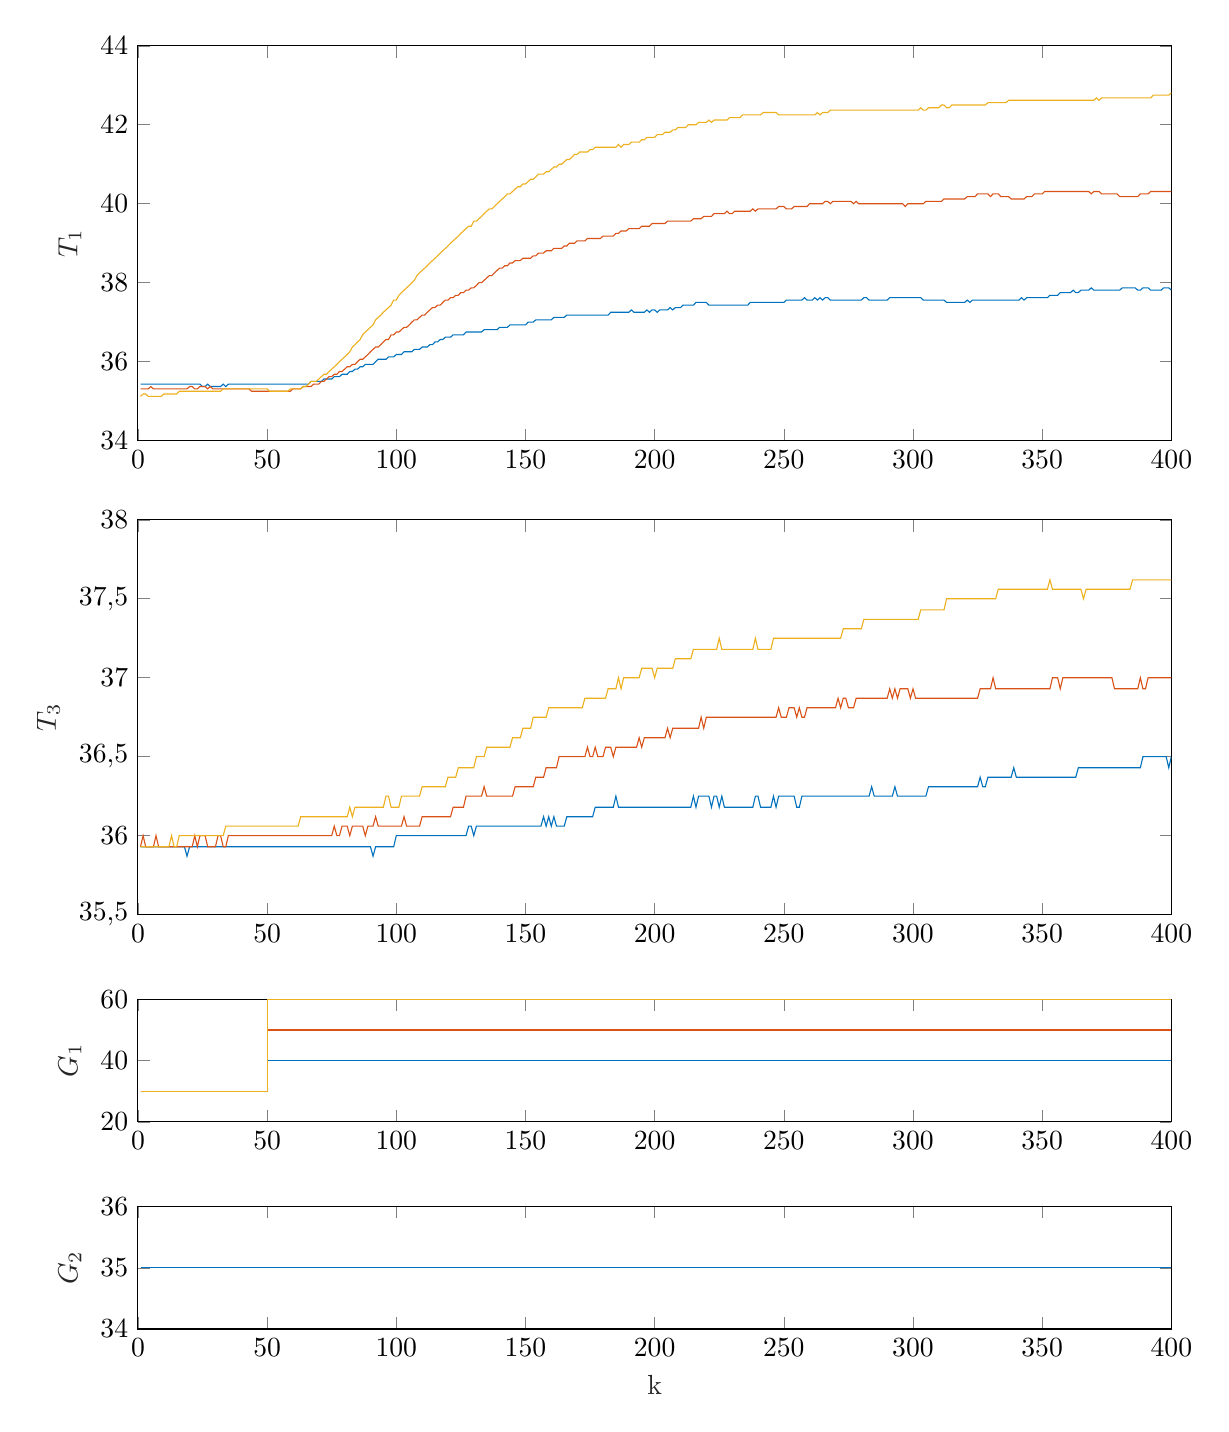
\begin{tikzpicture}

\begin{axis}[%
width=5.167in,
height=0.612in,
at={(0.646in,0.494in)},
scale only axis,
xmin=0,
xmax=400,
xtick={0,50,100,150,200,250,300,350,400},
xlabel style={font=\color{white!15!black}},
xlabel={k},
ymin=34,
ymax=36,
ytick={34,35,36},
ylabel style={font=\color{white!15!black}},
ylabel={$\text{G}_\text{2}$},
axis background/.style={fill=white}
]
\addplot[const plot, color=mycolor1, forget plot] table[row sep=crcr] {%
1	35\\
2	35\\
3	35\\
4	35\\
5	35\\
6	35\\
7	35\\
8	35\\
9	35\\
10	35\\
11	35\\
12	35\\
13	35\\
14	35\\
15	35\\
16	35\\
17	35\\
18	35\\
19	35\\
20	35\\
21	35\\
22	35\\
23	35\\
24	35\\
25	35\\
26	35\\
27	35\\
28	35\\
29	35\\
30	35\\
31	35\\
32	35\\
33	35\\
34	35\\
35	35\\
36	35\\
37	35\\
38	35\\
39	35\\
40	35\\
41	35\\
42	35\\
43	35\\
44	35\\
45	35\\
46	35\\
47	35\\
48	35\\
49	35\\
50	35\\
51	35\\
52	35\\
53	35\\
54	35\\
55	35\\
56	35\\
57	35\\
58	35\\
59	35\\
60	35\\
61	35\\
62	35\\
63	35\\
64	35\\
65	35\\
66	35\\
67	35\\
68	35\\
69	35\\
70	35\\
71	35\\
72	35\\
73	35\\
74	35\\
75	35\\
76	35\\
77	35\\
78	35\\
79	35\\
80	35\\
81	35\\
82	35\\
83	35\\
84	35\\
85	35\\
86	35\\
87	35\\
88	35\\
89	35\\
90	35\\
91	35\\
92	35\\
93	35\\
94	35\\
95	35\\
96	35\\
97	35\\
98	35\\
99	35\\
100	35\\
101	35\\
102	35\\
103	35\\
104	35\\
105	35\\
106	35\\
107	35\\
108	35\\
109	35\\
110	35\\
111	35\\
112	35\\
113	35\\
114	35\\
115	35\\
116	35\\
117	35\\
118	35\\
119	35\\
120	35\\
121	35\\
122	35\\
123	35\\
124	35\\
125	35\\
126	35\\
127	35\\
128	35\\
129	35\\
130	35\\
131	35\\
132	35\\
133	35\\
134	35\\
135	35\\
136	35\\
137	35\\
138	35\\
139	35\\
140	35\\
141	35\\
142	35\\
143	35\\
144	35\\
145	35\\
146	35\\
147	35\\
148	35\\
149	35\\
150	35\\
151	35\\
152	35\\
153	35\\
154	35\\
155	35\\
156	35\\
157	35\\
158	35\\
159	35\\
160	35\\
161	35\\
162	35\\
163	35\\
164	35\\
165	35\\
166	35\\
167	35\\
168	35\\
169	35\\
170	35\\
171	35\\
172	35\\
173	35\\
174	35\\
175	35\\
176	35\\
177	35\\
178	35\\
179	35\\
180	35\\
181	35\\
182	35\\
183	35\\
184	35\\
185	35\\
186	35\\
187	35\\
188	35\\
189	35\\
190	35\\
191	35\\
192	35\\
193	35\\
194	35\\
195	35\\
196	35\\
197	35\\
198	35\\
199	35\\
200	35\\
201	35\\
202	35\\
203	35\\
204	35\\
205	35\\
206	35\\
207	35\\
208	35\\
209	35\\
210	35\\
211	35\\
212	35\\
213	35\\
214	35\\
215	35\\
216	35\\
217	35\\
218	35\\
219	35\\
220	35\\
221	35\\
222	35\\
223	35\\
224	35\\
225	35\\
226	35\\
227	35\\
228	35\\
229	35\\
230	35\\
231	35\\
232	35\\
233	35\\
234	35\\
235	35\\
236	35\\
237	35\\
238	35\\
239	35\\
240	35\\
241	35\\
242	35\\
243	35\\
244	35\\
245	35\\
246	35\\
247	35\\
248	35\\
249	35\\
250	35\\
251	35\\
252	35\\
253	35\\
254	35\\
255	35\\
256	35\\
257	35\\
258	35\\
259	35\\
260	35\\
261	35\\
262	35\\
263	35\\
264	35\\
265	35\\
266	35\\
267	35\\
268	35\\
269	35\\
270	35\\
271	35\\
272	35\\
273	35\\
274	35\\
275	35\\
276	35\\
277	35\\
278	35\\
279	35\\
280	35\\
281	35\\
282	35\\
283	35\\
284	35\\
285	35\\
286	35\\
287	35\\
288	35\\
289	35\\
290	35\\
291	35\\
292	35\\
293	35\\
294	35\\
295	35\\
296	35\\
297	35\\
298	35\\
299	35\\
300	35\\
301	35\\
302	35\\
303	35\\
304	35\\
305	35\\
306	35\\
307	35\\
308	35\\
309	35\\
310	35\\
311	35\\
312	35\\
313	35\\
314	35\\
315	35\\
316	35\\
317	35\\
318	35\\
319	35\\
320	35\\
321	35\\
322	35\\
323	35\\
324	35\\
325	35\\
326	35\\
327	35\\
328	35\\
329	35\\
330	35\\
331	35\\
332	35\\
333	35\\
334	35\\
335	35\\
336	35\\
337	35\\
338	35\\
339	35\\
340	35\\
341	35\\
342	35\\
343	35\\
344	35\\
345	35\\
346	35\\
347	35\\
348	35\\
349	35\\
350	35\\
351	35\\
352	35\\
353	35\\
354	35\\
355	35\\
356	35\\
357	35\\
358	35\\
359	35\\
360	35\\
361	35\\
362	35\\
363	35\\
364	35\\
365	35\\
366	35\\
367	35\\
368	35\\
369	35\\
370	35\\
371	35\\
372	35\\
373	35\\
374	35\\
375	35\\
376	35\\
377	35\\
378	35\\
379	35\\
380	35\\
381	35\\
382	35\\
383	35\\
384	35\\
385	35\\
386	35\\
387	35\\
388	35\\
389	35\\
390	35\\
391	35\\
392	35\\
393	35\\
394	35\\
395	35\\
396	35\\
397	35\\
398	35\\
399	35\\
400	35\\
};
\end{axis}

\begin{axis}[%
width=5.167in,
height=0.612in,
at={(0.646in,1.53in)},
scale only axis,
xmin=0,
xmax=400,
xtick={0,50,100,150,200,250,300,350,400},
ymin=20,
ymax=60,
ytick={20,40,60},
ylabel style={font=\color{white!15!black}},
ylabel={$\text{G}_\text{1}$},
axis background/.style={fill=white}
]
\addplot[const plot, color=mycolor1, forget plot] table[row sep=crcr] {%
1	30\\
2	30\\
3	30\\
4	30\\
5	30\\
6	30\\
7	30\\
8	30\\
9	30\\
10	30\\
11	30\\
12	30\\
13	30\\
14	30\\
15	30\\
16	30\\
17	30\\
18	30\\
19	30\\
20	30\\
21	30\\
22	30\\
23	30\\
24	30\\
25	30\\
26	30\\
27	30\\
28	30\\
29	30\\
30	30\\
31	30\\
32	30\\
33	30\\
34	30\\
35	30\\
36	30\\
37	30\\
38	30\\
39	30\\
40	30\\
41	30\\
42	30\\
43	30\\
44	30\\
45	30\\
46	30\\
47	30\\
48	30\\
49	30\\
50	40\\
51	40\\
52	40\\
53	40\\
54	40\\
55	40\\
56	40\\
57	40\\
58	40\\
59	40\\
60	40\\
61	40\\
62	40\\
63	40\\
64	40\\
65	40\\
66	40\\
67	40\\
68	40\\
69	40\\
70	40\\
71	40\\
72	40\\
73	40\\
74	40\\
75	40\\
76	40\\
77	40\\
78	40\\
79	40\\
80	40\\
81	40\\
82	40\\
83	40\\
84	40\\
85	40\\
86	40\\
87	40\\
88	40\\
89	40\\
90	40\\
91	40\\
92	40\\
93	40\\
94	40\\
95	40\\
96	40\\
97	40\\
98	40\\
99	40\\
100	40\\
101	40\\
102	40\\
103	40\\
104	40\\
105	40\\
106	40\\
107	40\\
108	40\\
109	40\\
110	40\\
111	40\\
112	40\\
113	40\\
114	40\\
115	40\\
116	40\\
117	40\\
118	40\\
119	40\\
120	40\\
121	40\\
122	40\\
123	40\\
124	40\\
125	40\\
126	40\\
127	40\\
128	40\\
129	40\\
130	40\\
131	40\\
132	40\\
133	40\\
134	40\\
135	40\\
136	40\\
137	40\\
138	40\\
139	40\\
140	40\\
141	40\\
142	40\\
143	40\\
144	40\\
145	40\\
146	40\\
147	40\\
148	40\\
149	40\\
150	40\\
151	40\\
152	40\\
153	40\\
154	40\\
155	40\\
156	40\\
157	40\\
158	40\\
159	40\\
160	40\\
161	40\\
162	40\\
163	40\\
164	40\\
165	40\\
166	40\\
167	40\\
168	40\\
169	40\\
170	40\\
171	40\\
172	40\\
173	40\\
174	40\\
175	40\\
176	40\\
177	40\\
178	40\\
179	40\\
180	40\\
181	40\\
182	40\\
183	40\\
184	40\\
185	40\\
186	40\\
187	40\\
188	40\\
189	40\\
190	40\\
191	40\\
192	40\\
193	40\\
194	40\\
195	40\\
196	40\\
197	40\\
198	40\\
199	40\\
200	40\\
201	40\\
202	40\\
203	40\\
204	40\\
205	40\\
206	40\\
207	40\\
208	40\\
209	40\\
210	40\\
211	40\\
212	40\\
213	40\\
214	40\\
215	40\\
216	40\\
217	40\\
218	40\\
219	40\\
220	40\\
221	40\\
222	40\\
223	40\\
224	40\\
225	40\\
226	40\\
227	40\\
228	40\\
229	40\\
230	40\\
231	40\\
232	40\\
233	40\\
234	40\\
235	40\\
236	40\\
237	40\\
238	40\\
239	40\\
240	40\\
241	40\\
242	40\\
243	40\\
244	40\\
245	40\\
246	40\\
247	40\\
248	40\\
249	40\\
250	40\\
251	40\\
252	40\\
253	40\\
254	40\\
255	40\\
256	40\\
257	40\\
258	40\\
259	40\\
260	40\\
261	40\\
262	40\\
263	40\\
264	40\\
265	40\\
266	40\\
267	40\\
268	40\\
269	40\\
270	40\\
271	40\\
272	40\\
273	40\\
274	40\\
275	40\\
276	40\\
277	40\\
278	40\\
279	40\\
280	40\\
281	40\\
282	40\\
283	40\\
284	40\\
285	40\\
286	40\\
287	40\\
288	40\\
289	40\\
290	40\\
291	40\\
292	40\\
293	40\\
294	40\\
295	40\\
296	40\\
297	40\\
298	40\\
299	40\\
300	40\\
301	40\\
302	40\\
303	40\\
304	40\\
305	40\\
306	40\\
307	40\\
308	40\\
309	40\\
310	40\\
311	40\\
312	40\\
313	40\\
314	40\\
315	40\\
316	40\\
317	40\\
318	40\\
319	40\\
320	40\\
321	40\\
322	40\\
323	40\\
324	40\\
325	40\\
326	40\\
327	40\\
328	40\\
329	40\\
330	40\\
331	40\\
332	40\\
333	40\\
334	40\\
335	40\\
336	40\\
337	40\\
338	40\\
339	40\\
340	40\\
341	40\\
342	40\\
343	40\\
344	40\\
345	40\\
346	40\\
347	40\\
348	40\\
349	40\\
350	40\\
351	40\\
352	40\\
353	40\\
354	40\\
355	40\\
356	40\\
357	40\\
358	40\\
359	40\\
360	40\\
361	40\\
362	40\\
363	40\\
364	40\\
365	40\\
366	40\\
367	40\\
368	40\\
369	40\\
370	40\\
371	40\\
372	40\\
373	40\\
374	40\\
375	40\\
376	40\\
377	40\\
378	40\\
379	40\\
380	40\\
381	40\\
382	40\\
383	40\\
384	40\\
385	40\\
386	40\\
387	40\\
388	40\\
389	40\\
390	40\\
391	40\\
392	40\\
393	40\\
394	40\\
395	40\\
396	40\\
397	40\\
398	40\\
399	40\\
400	40\\
};
\addplot[const plot, color=mycolor2, forget plot] table[row sep=crcr] {%
1	30\\
2	30\\
3	30\\
4	30\\
5	30\\
6	30\\
7	30\\
8	30\\
9	30\\
10	30\\
11	30\\
12	30\\
13	30\\
14	30\\
15	30\\
16	30\\
17	30\\
18	30\\
19	30\\
20	30\\
21	30\\
22	30\\
23	30\\
24	30\\
25	30\\
26	30\\
27	30\\
28	30\\
29	30\\
30	30\\
31	30\\
32	30\\
33	30\\
34	30\\
35	30\\
36	30\\
37	30\\
38	30\\
39	30\\
40	30\\
41	30\\
42	30\\
43	30\\
44	30\\
45	30\\
46	30\\
47	30\\
48	30\\
49	30\\
50	50\\
51	50\\
52	50\\
53	50\\
54	50\\
55	50\\
56	50\\
57	50\\
58	50\\
59	50\\
60	50\\
61	50\\
62	50\\
63	50\\
64	50\\
65	50\\
66	50\\
67	50\\
68	50\\
69	50\\
70	50\\
71	50\\
72	50\\
73	50\\
74	50\\
75	50\\
76	50\\
77	50\\
78	50\\
79	50\\
80	50\\
81	50\\
82	50\\
83	50\\
84	50\\
85	50\\
86	50\\
87	50\\
88	50\\
89	50\\
90	50\\
91	50\\
92	50\\
93	50\\
94	50\\
95	50\\
96	50\\
97	50\\
98	50\\
99	50\\
100	50\\
101	50\\
102	50\\
103	50\\
104	50\\
105	50\\
106	50\\
107	50\\
108	50\\
109	50\\
110	50\\
111	50\\
112	50\\
113	50\\
114	50\\
115	50\\
116	50\\
117	50\\
118	50\\
119	50\\
120	50\\
121	50\\
122	50\\
123	50\\
124	50\\
125	50\\
126	50\\
127	50\\
128	50\\
129	50\\
130	50\\
131	50\\
132	50\\
133	50\\
134	50\\
135	50\\
136	50\\
137	50\\
138	50\\
139	50\\
140	50\\
141	50\\
142	50\\
143	50\\
144	50\\
145	50\\
146	50\\
147	50\\
148	50\\
149	50\\
150	50\\
151	50\\
152	50\\
153	50\\
154	50\\
155	50\\
156	50\\
157	50\\
158	50\\
159	50\\
160	50\\
161	50\\
162	50\\
163	50\\
164	50\\
165	50\\
166	50\\
167	50\\
168	50\\
169	50\\
170	50\\
171	50\\
172	50\\
173	50\\
174	50\\
175	50\\
176	50\\
177	50\\
178	50\\
179	50\\
180	50\\
181	50\\
182	50\\
183	50\\
184	50\\
185	50\\
186	50\\
187	50\\
188	50\\
189	50\\
190	50\\
191	50\\
192	50\\
193	50\\
194	50\\
195	50\\
196	50\\
197	50\\
198	50\\
199	50\\
200	50\\
201	50\\
202	50\\
203	50\\
204	50\\
205	50\\
206	50\\
207	50\\
208	50\\
209	50\\
210	50\\
211	50\\
212	50\\
213	50\\
214	50\\
215	50\\
216	50\\
217	50\\
218	50\\
219	50\\
220	50\\
221	50\\
222	50\\
223	50\\
224	50\\
225	50\\
226	50\\
227	50\\
228	50\\
229	50\\
230	50\\
231	50\\
232	50\\
233	50\\
234	50\\
235	50\\
236	50\\
237	50\\
238	50\\
239	50\\
240	50\\
241	50\\
242	50\\
243	50\\
244	50\\
245	50\\
246	50\\
247	50\\
248	50\\
249	50\\
250	50\\
251	50\\
252	50\\
253	50\\
254	50\\
255	50\\
256	50\\
257	50\\
258	50\\
259	50\\
260	50\\
261	50\\
262	50\\
263	50\\
264	50\\
265	50\\
266	50\\
267	50\\
268	50\\
269	50\\
270	50\\
271	50\\
272	50\\
273	50\\
274	50\\
275	50\\
276	50\\
277	50\\
278	50\\
279	50\\
280	50\\
281	50\\
282	50\\
283	50\\
284	50\\
285	50\\
286	50\\
287	50\\
288	50\\
289	50\\
290	50\\
291	50\\
292	50\\
293	50\\
294	50\\
295	50\\
296	50\\
297	50\\
298	50\\
299	50\\
300	50\\
301	50\\
302	50\\
303	50\\
304	50\\
305	50\\
306	50\\
307	50\\
308	50\\
309	50\\
310	50\\
311	50\\
312	50\\
313	50\\
314	50\\
315	50\\
316	50\\
317	50\\
318	50\\
319	50\\
320	50\\
321	50\\
322	50\\
323	50\\
324	50\\
325	50\\
326	50\\
327	50\\
328	50\\
329	50\\
330	50\\
331	50\\
332	50\\
333	50\\
334	50\\
335	50\\
336	50\\
337	50\\
338	50\\
339	50\\
340	50\\
341	50\\
342	50\\
343	50\\
344	50\\
345	50\\
346	50\\
347	50\\
348	50\\
349	50\\
350	50\\
351	50\\
352	50\\
353	50\\
354	50\\
355	50\\
356	50\\
357	50\\
358	50\\
359	50\\
360	50\\
361	50\\
362	50\\
363	50\\
364	50\\
365	50\\
366	50\\
367	50\\
368	50\\
369	50\\
370	50\\
371	50\\
372	50\\
373	50\\
374	50\\
375	50\\
376	50\\
377	50\\
378	50\\
379	50\\
380	50\\
381	50\\
382	50\\
383	50\\
384	50\\
385	50\\
386	50\\
387	50\\
388	50\\
389	50\\
390	50\\
391	50\\
392	50\\
393	50\\
394	50\\
395	50\\
396	50\\
397	50\\
398	50\\
399	50\\
400	50\\
};
\addplot[const plot, color=mycolor3, forget plot] table[row sep=crcr] {%
1	30\\
2	30\\
3	30\\
4	30\\
5	30\\
6	30\\
7	30\\
8	30\\
9	30\\
10	30\\
11	30\\
12	30\\
13	30\\
14	30\\
15	30\\
16	30\\
17	30\\
18	30\\
19	30\\
20	30\\
21	30\\
22	30\\
23	30\\
24	30\\
25	30\\
26	30\\
27	30\\
28	30\\
29	30\\
30	30\\
31	30\\
32	30\\
33	30\\
34	30\\
35	30\\
36	30\\
37	30\\
38	30\\
39	30\\
40	30\\
41	30\\
42	30\\
43	30\\
44	30\\
45	30\\
46	30\\
47	30\\
48	30\\
49	30\\
50	60\\
51	60\\
52	60\\
53	60\\
54	60\\
55	60\\
56	60\\
57	60\\
58	60\\
59	60\\
60	60\\
61	60\\
62	60\\
63	60\\
64	60\\
65	60\\
66	60\\
67	60\\
68	60\\
69	60\\
70	60\\
71	60\\
72	60\\
73	60\\
74	60\\
75	60\\
76	60\\
77	60\\
78	60\\
79	60\\
80	60\\
81	60\\
82	60\\
83	60\\
84	60\\
85	60\\
86	60\\
87	60\\
88	60\\
89	60\\
90	60\\
91	60\\
92	60\\
93	60\\
94	60\\
95	60\\
96	60\\
97	60\\
98	60\\
99	60\\
100	60\\
101	60\\
102	60\\
103	60\\
104	60\\
105	60\\
106	60\\
107	60\\
108	60\\
109	60\\
110	60\\
111	60\\
112	60\\
113	60\\
114	60\\
115	60\\
116	60\\
117	60\\
118	60\\
119	60\\
120	60\\
121	60\\
122	60\\
123	60\\
124	60\\
125	60\\
126	60\\
127	60\\
128	60\\
129	60\\
130	60\\
131	60\\
132	60\\
133	60\\
134	60\\
135	60\\
136	60\\
137	60\\
138	60\\
139	60\\
140	60\\
141	60\\
142	60\\
143	60\\
144	60\\
145	60\\
146	60\\
147	60\\
148	60\\
149	60\\
150	60\\
151	60\\
152	60\\
153	60\\
154	60\\
155	60\\
156	60\\
157	60\\
158	60\\
159	60\\
160	60\\
161	60\\
162	60\\
163	60\\
164	60\\
165	60\\
166	60\\
167	60\\
168	60\\
169	60\\
170	60\\
171	60\\
172	60\\
173	60\\
174	60\\
175	60\\
176	60\\
177	60\\
178	60\\
179	60\\
180	60\\
181	60\\
182	60\\
183	60\\
184	60\\
185	60\\
186	60\\
187	60\\
188	60\\
189	60\\
190	60\\
191	60\\
192	60\\
193	60\\
194	60\\
195	60\\
196	60\\
197	60\\
198	60\\
199	60\\
200	60\\
201	60\\
202	60\\
203	60\\
204	60\\
205	60\\
206	60\\
207	60\\
208	60\\
209	60\\
210	60\\
211	60\\
212	60\\
213	60\\
214	60\\
215	60\\
216	60\\
217	60\\
218	60\\
219	60\\
220	60\\
221	60\\
222	60\\
223	60\\
224	60\\
225	60\\
226	60\\
227	60\\
228	60\\
229	60\\
230	60\\
231	60\\
232	60\\
233	60\\
234	60\\
235	60\\
236	60\\
237	60\\
238	60\\
239	60\\
240	60\\
241	60\\
242	60\\
243	60\\
244	60\\
245	60\\
246	60\\
247	60\\
248	60\\
249	60\\
250	60\\
251	60\\
252	60\\
253	60\\
254	60\\
255	60\\
256	60\\
257	60\\
258	60\\
259	60\\
260	60\\
261	60\\
262	60\\
263	60\\
264	60\\
265	60\\
266	60\\
267	60\\
268	60\\
269	60\\
270	60\\
271	60\\
272	60\\
273	60\\
274	60\\
275	60\\
276	60\\
277	60\\
278	60\\
279	60\\
280	60\\
281	60\\
282	60\\
283	60\\
284	60\\
285	60\\
286	60\\
287	60\\
288	60\\
289	60\\
290	60\\
291	60\\
292	60\\
293	60\\
294	60\\
295	60\\
296	60\\
297	60\\
298	60\\
299	60\\
300	60\\
301	60\\
302	60\\
303	60\\
304	60\\
305	60\\
306	60\\
307	60\\
308	60\\
309	60\\
310	60\\
311	60\\
312	60\\
313	60\\
314	60\\
315	60\\
316	60\\
317	60\\
318	60\\
319	60\\
320	60\\
321	60\\
322	60\\
323	60\\
324	60\\
325	60\\
326	60\\
327	60\\
328	60\\
329	60\\
330	60\\
331	60\\
332	60\\
333	60\\
334	60\\
335	60\\
336	60\\
337	60\\
338	60\\
339	60\\
340	60\\
341	60\\
342	60\\
343	60\\
344	60\\
345	60\\
346	60\\
347	60\\
348	60\\
349	60\\
350	60\\
351	60\\
352	60\\
353	60\\
354	60\\
355	60\\
356	60\\
357	60\\
358	60\\
359	60\\
360	60\\
361	60\\
362	60\\
363	60\\
364	60\\
365	60\\
366	60\\
367	60\\
368	60\\
369	60\\
370	60\\
371	60\\
372	60\\
373	60\\
374	60\\
375	60\\
376	60\\
377	60\\
378	60\\
379	60\\
380	60\\
381	60\\
382	60\\
383	60\\
384	60\\
385	60\\
386	60\\
387	60\\
388	60\\
389	60\\
390	60\\
391	60\\
392	60\\
393	60\\
394	60\\
395	60\\
396	60\\
397	60\\
398	60\\
399	60\\
400	60\\
};
\end{axis}

\begin{axis}[%
width=5.167in,
height=1.974in,
at={(0.646in,2.566in)},
scale only axis,
xmin=0,
xmax=400,
xtick={0,50,100,150,200,250,300,350,400},
ymin=35.5,
ymax=38,
ytick={35.5,36,36.5,37,37.5,38},
yticklabels={{35,5},{36},{36,5},{37},{37,5},{38}},
ylabel style={font=\color{white!15!black}},
ylabel={$\text{T}_\text{3}$},
axis background/.style={fill=white}
]
\addplot [color=mycolor1, forget plot]
  table[row sep=crcr]{%
1	35.93\\
2	35.93\\
3	35.93\\
4	35.93\\
5	35.93\\
6	35.93\\
7	35.93\\
8	35.93\\
9	35.93\\
10	35.93\\
11	35.93\\
12	35.93\\
13	35.93\\
14	35.93\\
15	35.93\\
16	35.93\\
17	35.93\\
18	35.93\\
19	35.87\\
20	35.93\\
21	35.93\\
22	35.93\\
23	35.93\\
24	35.93\\
25	35.93\\
26	35.93\\
27	35.93\\
28	35.93\\
29	35.93\\
30	35.93\\
31	35.93\\
32	35.93\\
33	35.93\\
34	35.93\\
35	35.93\\
36	35.93\\
37	35.93\\
38	35.93\\
39	35.93\\
40	35.93\\
41	35.93\\
42	35.93\\
43	35.93\\
44	35.93\\
45	35.93\\
46	35.93\\
47	35.93\\
48	35.93\\
49	35.93\\
50	35.93\\
51	35.93\\
52	35.93\\
53	35.93\\
54	35.93\\
55	35.93\\
56	35.93\\
57	35.93\\
58	35.93\\
59	35.93\\
60	35.93\\
61	35.93\\
62	35.93\\
63	35.93\\
64	35.93\\
65	35.93\\
66	35.93\\
67	35.93\\
68	35.93\\
69	35.93\\
70	35.93\\
71	35.93\\
72	35.93\\
73	35.93\\
74	35.93\\
75	35.93\\
76	35.93\\
77	35.93\\
78	35.93\\
79	35.93\\
80	35.93\\
81	35.93\\
82	35.93\\
83	35.93\\
84	35.93\\
85	35.93\\
86	35.93\\
87	35.93\\
88	35.93\\
89	35.93\\
90	35.93\\
91	35.87\\
92	35.93\\
93	35.93\\
94	35.93\\
95	35.93\\
96	35.93\\
97	35.93\\
98	35.93\\
99	35.93\\
100	36\\
101	36\\
102	36\\
103	36\\
104	36\\
105	36\\
106	36\\
107	36\\
108	36\\
109	36\\
110	36\\
111	36\\
112	36\\
113	36\\
114	36\\
115	36\\
116	36\\
117	36\\
118	36\\
119	36\\
120	36\\
121	36\\
122	36\\
123	36\\
124	36\\
125	36\\
126	36\\
127	36\\
128	36.06\\
129	36.06\\
130	36\\
131	36.06\\
132	36.06\\
133	36.06\\
134	36.06\\
135	36.06\\
136	36.06\\
137	36.06\\
138	36.06\\
139	36.06\\
140	36.06\\
141	36.06\\
142	36.06\\
143	36.06\\
144	36.06\\
145	36.06\\
146	36.06\\
147	36.06\\
148	36.06\\
149	36.06\\
150	36.06\\
151	36.06\\
152	36.06\\
153	36.06\\
154	36.06\\
155	36.06\\
156	36.06\\
157	36.12\\
158	36.06\\
159	36.12\\
160	36.06\\
161	36.12\\
162	36.06\\
163	36.06\\
164	36.06\\
165	36.06\\
166	36.12\\
167	36.12\\
168	36.12\\
169	36.12\\
170	36.12\\
171	36.12\\
172	36.12\\
173	36.12\\
174	36.12\\
175	36.12\\
176	36.12\\
177	36.18\\
178	36.18\\
179	36.18\\
180	36.18\\
181	36.18\\
182	36.18\\
183	36.18\\
184	36.18\\
185	36.25\\
186	36.18\\
187	36.18\\
188	36.18\\
189	36.18\\
190	36.18\\
191	36.18\\
192	36.18\\
193	36.18\\
194	36.18\\
195	36.18\\
196	36.18\\
197	36.18\\
198	36.18\\
199	36.18\\
200	36.18\\
201	36.18\\
202	36.18\\
203	36.18\\
204	36.18\\
205	36.18\\
206	36.18\\
207	36.18\\
208	36.18\\
209	36.18\\
210	36.18\\
211	36.18\\
212	36.18\\
213	36.18\\
214	36.18\\
215	36.25\\
216	36.18\\
217	36.25\\
218	36.25\\
219	36.25\\
220	36.25\\
221	36.25\\
222	36.18\\
223	36.25\\
224	36.25\\
225	36.18\\
226	36.25\\
227	36.18\\
228	36.18\\
229	36.18\\
230	36.18\\
231	36.18\\
232	36.18\\
233	36.18\\
234	36.18\\
235	36.18\\
236	36.18\\
237	36.18\\
238	36.18\\
239	36.25\\
240	36.25\\
241	36.18\\
242	36.18\\
243	36.18\\
244	36.18\\
245	36.18\\
246	36.25\\
247	36.18\\
248	36.25\\
249	36.25\\
250	36.25\\
251	36.25\\
252	36.25\\
253	36.25\\
254	36.25\\
255	36.18\\
256	36.18\\
257	36.25\\
258	36.25\\
259	36.25\\
260	36.25\\
261	36.25\\
262	36.25\\
263	36.25\\
264	36.25\\
265	36.25\\
266	36.25\\
267	36.25\\
268	36.25\\
269	36.25\\
270	36.25\\
271	36.25\\
272	36.25\\
273	36.25\\
274	36.25\\
275	36.25\\
276	36.25\\
277	36.25\\
278	36.25\\
279	36.25\\
280	36.25\\
281	36.25\\
282	36.25\\
283	36.25\\
284	36.31\\
285	36.25\\
286	36.25\\
287	36.25\\
288	36.25\\
289	36.25\\
290	36.25\\
291	36.25\\
292	36.25\\
293	36.31\\
294	36.25\\
295	36.25\\
296	36.25\\
297	36.25\\
298	36.25\\
299	36.25\\
300	36.25\\
301	36.25\\
302	36.25\\
303	36.25\\
304	36.25\\
305	36.25\\
306	36.31\\
307	36.31\\
308	36.31\\
309	36.31\\
310	36.31\\
311	36.31\\
312	36.31\\
313	36.31\\
314	36.31\\
315	36.31\\
316	36.31\\
317	36.31\\
318	36.31\\
319	36.31\\
320	36.31\\
321	36.31\\
322	36.31\\
323	36.31\\
324	36.31\\
325	36.31\\
326	36.37\\
327	36.31\\
328	36.31\\
329	36.37\\
330	36.37\\
331	36.37\\
332	36.37\\
333	36.37\\
334	36.37\\
335	36.37\\
336	36.37\\
337	36.37\\
338	36.37\\
339	36.43\\
340	36.37\\
341	36.37\\
342	36.37\\
343	36.37\\
344	36.37\\
345	36.37\\
346	36.37\\
347	36.37\\
348	36.37\\
349	36.37\\
350	36.37\\
351	36.37\\
352	36.37\\
353	36.37\\
354	36.37\\
355	36.37\\
356	36.37\\
357	36.37\\
358	36.37\\
359	36.37\\
360	36.37\\
361	36.37\\
362	36.37\\
363	36.37\\
364	36.43\\
365	36.43\\
366	36.43\\
367	36.43\\
368	36.43\\
369	36.43\\
370	36.43\\
371	36.43\\
372	36.43\\
373	36.43\\
374	36.43\\
375	36.43\\
376	36.43\\
377	36.43\\
378	36.43\\
379	36.43\\
380	36.43\\
381	36.43\\
382	36.43\\
383	36.43\\
384	36.43\\
385	36.43\\
386	36.43\\
387	36.43\\
388	36.43\\
389	36.5\\
390	36.5\\
391	36.5\\
392	36.5\\
393	36.5\\
394	36.5\\
395	36.5\\
396	36.5\\
397	36.5\\
398	36.5\\
399	36.43\\
400	36.5\\
};
\addplot [color=mycolor2, forget plot]
  table[row sep=crcr]{%
1	35.93\\
2	36\\
3	35.93\\
4	35.93\\
5	35.93\\
6	35.93\\
7	36\\
8	35.93\\
9	35.93\\
10	35.93\\
11	35.93\\
12	35.93\\
13	35.93\\
14	35.93\\
15	35.93\\
16	35.93\\
17	35.93\\
18	35.93\\
19	35.93\\
20	35.93\\
21	35.93\\
22	36\\
23	35.93\\
24	36\\
25	36\\
26	36\\
27	35.93\\
28	35.93\\
29	35.93\\
30	35.93\\
31	36\\
32	36\\
33	35.93\\
34	35.93\\
35	36\\
36	36\\
37	36\\
38	36\\
39	36\\
40	36\\
41	36\\
42	36\\
43	36\\
44	36\\
45	36\\
46	36\\
47	36\\
48	36\\
49	36\\
50	36\\
51	36\\
52	36\\
53	36\\
54	36\\
55	36\\
56	36\\
57	36\\
58	36\\
59	36\\
60	36\\
61	36\\
62	36\\
63	36\\
64	36\\
65	36\\
66	36\\
67	36\\
68	36\\
69	36\\
70	36\\
71	36\\
72	36\\
73	36\\
74	36\\
75	36\\
76	36.06\\
77	36\\
78	36\\
79	36.06\\
80	36.06\\
81	36.06\\
82	36\\
83	36.06\\
84	36.06\\
85	36.06\\
86	36.06\\
87	36.06\\
88	36\\
89	36.06\\
90	36.06\\
91	36.06\\
92	36.12\\
93	36.06\\
94	36.06\\
95	36.06\\
96	36.06\\
97	36.06\\
98	36.06\\
99	36.06\\
100	36.06\\
101	36.06\\
102	36.06\\
103	36.12\\
104	36.06\\
105	36.06\\
106	36.06\\
107	36.06\\
108	36.06\\
109	36.06\\
110	36.12\\
111	36.12\\
112	36.12\\
113	36.12\\
114	36.12\\
115	36.12\\
116	36.12\\
117	36.12\\
118	36.12\\
119	36.12\\
120	36.12\\
121	36.12\\
122	36.18\\
123	36.18\\
124	36.18\\
125	36.18\\
126	36.18\\
127	36.25\\
128	36.25\\
129	36.25\\
130	36.25\\
131	36.25\\
132	36.25\\
133	36.25\\
134	36.31\\
135	36.25\\
136	36.25\\
137	36.25\\
138	36.25\\
139	36.25\\
140	36.25\\
141	36.25\\
142	36.25\\
143	36.25\\
144	36.25\\
145	36.25\\
146	36.31\\
147	36.31\\
148	36.31\\
149	36.31\\
150	36.31\\
151	36.31\\
152	36.31\\
153	36.31\\
154	36.37\\
155	36.37\\
156	36.37\\
157	36.37\\
158	36.43\\
159	36.43\\
160	36.43\\
161	36.43\\
162	36.43\\
163	36.5\\
164	36.5\\
165	36.5\\
166	36.5\\
167	36.5\\
168	36.5\\
169	36.5\\
170	36.5\\
171	36.5\\
172	36.5\\
173	36.5\\
174	36.56\\
175	36.5\\
176	36.5\\
177	36.56\\
178	36.5\\
179	36.5\\
180	36.5\\
181	36.56\\
182	36.56\\
183	36.56\\
184	36.5\\
185	36.56\\
186	36.56\\
187	36.56\\
188	36.56\\
189	36.56\\
190	36.56\\
191	36.56\\
192	36.56\\
193	36.56\\
194	36.62\\
195	36.56\\
196	36.62\\
197	36.62\\
198	36.62\\
199	36.62\\
200	36.62\\
201	36.62\\
202	36.62\\
203	36.62\\
204	36.62\\
205	36.68\\
206	36.62\\
207	36.68\\
208	36.68\\
209	36.68\\
210	36.68\\
211	36.68\\
212	36.68\\
213	36.68\\
214	36.68\\
215	36.68\\
216	36.68\\
217	36.68\\
218	36.75\\
219	36.68\\
220	36.75\\
221	36.75\\
222	36.75\\
223	36.75\\
224	36.75\\
225	36.75\\
226	36.75\\
227	36.75\\
228	36.75\\
229	36.75\\
230	36.75\\
231	36.75\\
232	36.75\\
233	36.75\\
234	36.75\\
235	36.75\\
236	36.75\\
237	36.75\\
238	36.75\\
239	36.75\\
240	36.75\\
241	36.75\\
242	36.75\\
243	36.75\\
244	36.75\\
245	36.75\\
246	36.75\\
247	36.75\\
248	36.81\\
249	36.75\\
250	36.75\\
251	36.75\\
252	36.81\\
253	36.81\\
254	36.81\\
255	36.75\\
256	36.81\\
257	36.75\\
258	36.75\\
259	36.81\\
260	36.81\\
261	36.81\\
262	36.81\\
263	36.81\\
264	36.81\\
265	36.81\\
266	36.81\\
267	36.81\\
268	36.81\\
269	36.81\\
270	36.81\\
271	36.87\\
272	36.81\\
273	36.87\\
274	36.87\\
275	36.81\\
276	36.81\\
277	36.81\\
278	36.87\\
279	36.87\\
280	36.87\\
281	36.87\\
282	36.87\\
283	36.87\\
284	36.87\\
285	36.87\\
286	36.87\\
287	36.87\\
288	36.87\\
289	36.87\\
290	36.87\\
291	36.93\\
292	36.87\\
293	36.93\\
294	36.87\\
295	36.93\\
296	36.93\\
297	36.93\\
298	36.93\\
299	36.87\\
300	36.93\\
301	36.87\\
302	36.87\\
303	36.87\\
304	36.87\\
305	36.87\\
306	36.87\\
307	36.87\\
308	36.87\\
309	36.87\\
310	36.87\\
311	36.87\\
312	36.87\\
313	36.87\\
314	36.87\\
315	36.87\\
316	36.87\\
317	36.87\\
318	36.87\\
319	36.87\\
320	36.87\\
321	36.87\\
322	36.87\\
323	36.87\\
324	36.87\\
325	36.87\\
326	36.93\\
327	36.93\\
328	36.93\\
329	36.93\\
330	36.93\\
331	37\\
332	36.93\\
333	36.93\\
334	36.93\\
335	36.93\\
336	36.93\\
337	36.93\\
338	36.93\\
339	36.93\\
340	36.93\\
341	36.93\\
342	36.93\\
343	36.93\\
344	36.93\\
345	36.93\\
346	36.93\\
347	36.93\\
348	36.93\\
349	36.93\\
350	36.93\\
351	36.93\\
352	36.93\\
353	36.93\\
354	37\\
355	37\\
356	37\\
357	36.93\\
358	37\\
359	37\\
360	37\\
361	37\\
362	37\\
363	37\\
364	37\\
365	37\\
366	37\\
367	37\\
368	37\\
369	37\\
370	37\\
371	37\\
372	37\\
373	37\\
374	37\\
375	37\\
376	37\\
377	37\\
378	36.93\\
379	36.93\\
380	36.93\\
381	36.93\\
382	36.93\\
383	36.93\\
384	36.93\\
385	36.93\\
386	36.93\\
387	36.93\\
388	37\\
389	36.93\\
390	36.93\\
391	37\\
392	37\\
393	37\\
394	37\\
395	37\\
396	37\\
397	37\\
398	37\\
399	37\\
400	37\\
};
\addplot [color=mycolor3, forget plot]
  table[row sep=crcr]{%
1	35.93\\
2	35.93\\
3	35.93\\
4	35.93\\
5	35.93\\
6	35.93\\
7	35.93\\
8	35.93\\
9	35.93\\
10	35.93\\
11	35.93\\
12	35.93\\
13	36\\
14	35.93\\
15	35.93\\
16	36\\
17	36\\
18	36\\
19	36\\
20	36\\
21	36\\
22	36\\
23	36\\
24	36\\
25	36\\
26	36\\
27	36\\
28	36\\
29	36\\
30	36\\
31	36\\
32	36\\
33	36\\
34	36.06\\
35	36.06\\
36	36.06\\
37	36.06\\
38	36.06\\
39	36.06\\
40	36.06\\
41	36.06\\
42	36.06\\
43	36.06\\
44	36.06\\
45	36.06\\
46	36.06\\
47	36.06\\
48	36.06\\
49	36.06\\
50	36.06\\
51	36.06\\
52	36.06\\
53	36.06\\
54	36.06\\
55	36.06\\
56	36.06\\
57	36.06\\
58	36.06\\
59	36.06\\
60	36.06\\
61	36.06\\
62	36.06\\
63	36.12\\
64	36.12\\
65	36.12\\
66	36.12\\
67	36.12\\
68	36.12\\
69	36.12\\
70	36.12\\
71	36.12\\
72	36.12\\
73	36.12\\
74	36.12\\
75	36.12\\
76	36.12\\
77	36.12\\
78	36.12\\
79	36.12\\
80	36.12\\
81	36.12\\
82	36.18\\
83	36.12\\
84	36.18\\
85	36.18\\
86	36.18\\
87	36.18\\
88	36.18\\
89	36.18\\
90	36.18\\
91	36.18\\
92	36.18\\
93	36.18\\
94	36.18\\
95	36.18\\
96	36.25\\
97	36.25\\
98	36.18\\
99	36.18\\
100	36.18\\
101	36.18\\
102	36.25\\
103	36.25\\
104	36.25\\
105	36.25\\
106	36.25\\
107	36.25\\
108	36.25\\
109	36.25\\
110	36.31\\
111	36.31\\
112	36.31\\
113	36.31\\
114	36.31\\
115	36.31\\
116	36.31\\
117	36.31\\
118	36.31\\
119	36.31\\
120	36.37\\
121	36.37\\
122	36.37\\
123	36.37\\
124	36.43\\
125	36.43\\
126	36.43\\
127	36.43\\
128	36.43\\
129	36.43\\
130	36.43\\
131	36.5\\
132	36.5\\
133	36.5\\
134	36.5\\
135	36.56\\
136	36.56\\
137	36.56\\
138	36.56\\
139	36.56\\
140	36.56\\
141	36.56\\
142	36.56\\
143	36.56\\
144	36.56\\
145	36.62\\
146	36.62\\
147	36.62\\
148	36.62\\
149	36.68\\
150	36.68\\
151	36.68\\
152	36.68\\
153	36.75\\
154	36.75\\
155	36.75\\
156	36.75\\
157	36.75\\
158	36.75\\
159	36.81\\
160	36.81\\
161	36.81\\
162	36.81\\
163	36.81\\
164	36.81\\
165	36.81\\
166	36.81\\
167	36.81\\
168	36.81\\
169	36.81\\
170	36.81\\
171	36.81\\
172	36.81\\
173	36.87\\
174	36.87\\
175	36.87\\
176	36.87\\
177	36.87\\
178	36.87\\
179	36.87\\
180	36.87\\
181	36.87\\
182	36.93\\
183	36.93\\
184	36.93\\
185	36.93\\
186	37\\
187	36.93\\
188	37\\
189	37\\
190	37\\
191	37\\
192	37\\
193	37\\
194	37\\
195	37.06\\
196	37.06\\
197	37.06\\
198	37.06\\
199	37.06\\
200	37\\
201	37.06\\
202	37.06\\
203	37.06\\
204	37.06\\
205	37.06\\
206	37.06\\
207	37.06\\
208	37.12\\
209	37.12\\
210	37.12\\
211	37.12\\
212	37.12\\
213	37.12\\
214	37.12\\
215	37.18\\
216	37.18\\
217	37.18\\
218	37.18\\
219	37.18\\
220	37.18\\
221	37.18\\
222	37.18\\
223	37.18\\
224	37.18\\
225	37.25\\
226	37.18\\
227	37.18\\
228	37.18\\
229	37.18\\
230	37.18\\
231	37.18\\
232	37.18\\
233	37.18\\
234	37.18\\
235	37.18\\
236	37.18\\
237	37.18\\
238	37.18\\
239	37.25\\
240	37.18\\
241	37.18\\
242	37.18\\
243	37.18\\
244	37.18\\
245	37.18\\
246	37.25\\
247	37.25\\
248	37.25\\
249	37.25\\
250	37.25\\
251	37.25\\
252	37.25\\
253	37.25\\
254	37.25\\
255	37.25\\
256	37.25\\
257	37.25\\
258	37.25\\
259	37.25\\
260	37.25\\
261	37.25\\
262	37.25\\
263	37.25\\
264	37.25\\
265	37.25\\
266	37.25\\
267	37.25\\
268	37.25\\
269	37.25\\
270	37.25\\
271	37.25\\
272	37.25\\
273	37.31\\
274	37.31\\
275	37.31\\
276	37.31\\
277	37.31\\
278	37.31\\
279	37.31\\
280	37.31\\
281	37.37\\
282	37.37\\
283	37.37\\
284	37.37\\
285	37.37\\
286	37.37\\
287	37.37\\
288	37.37\\
289	37.37\\
290	37.37\\
291	37.37\\
292	37.37\\
293	37.37\\
294	37.37\\
295	37.37\\
296	37.37\\
297	37.37\\
298	37.37\\
299	37.37\\
300	37.37\\
301	37.37\\
302	37.37\\
303	37.43\\
304	37.43\\
305	37.43\\
306	37.43\\
307	37.43\\
308	37.43\\
309	37.43\\
310	37.43\\
311	37.43\\
312	37.43\\
313	37.5\\
314	37.5\\
315	37.5\\
316	37.5\\
317	37.5\\
318	37.5\\
319	37.5\\
320	37.5\\
321	37.5\\
322	37.5\\
323	37.5\\
324	37.5\\
325	37.5\\
326	37.5\\
327	37.5\\
328	37.5\\
329	37.5\\
330	37.5\\
331	37.5\\
332	37.5\\
333	37.56\\
334	37.56\\
335	37.56\\
336	37.56\\
337	37.56\\
338	37.56\\
339	37.56\\
340	37.56\\
341	37.56\\
342	37.56\\
343	37.56\\
344	37.56\\
345	37.56\\
346	37.56\\
347	37.56\\
348	37.56\\
349	37.56\\
350	37.56\\
351	37.56\\
352	37.56\\
353	37.62\\
354	37.56\\
355	37.56\\
356	37.56\\
357	37.56\\
358	37.56\\
359	37.56\\
360	37.56\\
361	37.56\\
362	37.56\\
363	37.56\\
364	37.56\\
365	37.56\\
366	37.5\\
367	37.56\\
368	37.56\\
369	37.56\\
370	37.56\\
371	37.56\\
372	37.56\\
373	37.56\\
374	37.56\\
375	37.56\\
376	37.56\\
377	37.56\\
378	37.56\\
379	37.56\\
380	37.56\\
381	37.56\\
382	37.56\\
383	37.56\\
384	37.56\\
385	37.62\\
386	37.62\\
387	37.62\\
388	37.62\\
389	37.62\\
390	37.62\\
391	37.62\\
392	37.62\\
393	37.62\\
394	37.62\\
395	37.62\\
396	37.62\\
397	37.62\\
398	37.62\\
399	37.62\\
400	37.62\\
};
\end{axis}

\begin{axis}[%
width=5.167in,
height=1.974in,
at={(0.646in,4.936in)},
scale only axis,
xmin=0,
xmax=400,
xtick={0,50,100,150,200,250,300,350,400},
ymin=34,
ymax=44,
ytick={34,36,38,40,42,44},
ylabel style={font=\color{white!15!black}},
ylabel={$\text{T}_\text{1}$},
axis background/.style={fill=white}
]
\addplot [color=mycolor1, forget plot]
  table[row sep=crcr]{%
1	35.43\\
2	35.43\\
3	35.43\\
4	35.43\\
5	35.43\\
6	35.43\\
7	35.43\\
8	35.43\\
9	35.43\\
10	35.43\\
11	35.43\\
12	35.43\\
13	35.43\\
14	35.43\\
15	35.43\\
16	35.43\\
17	35.43\\
18	35.43\\
19	35.43\\
20	35.43\\
21	35.43\\
22	35.43\\
23	35.43\\
24	35.43\\
25	35.37\\
26	35.37\\
27	35.43\\
28	35.37\\
29	35.37\\
30	35.37\\
31	35.37\\
32	35.37\\
33	35.43\\
34	35.37\\
35	35.43\\
36	35.43\\
37	35.43\\
38	35.43\\
39	35.43\\
40	35.43\\
41	35.43\\
42	35.43\\
43	35.43\\
44	35.43\\
45	35.43\\
46	35.43\\
47	35.43\\
48	35.43\\
49	35.43\\
50	35.43\\
51	35.43\\
52	35.43\\
53	35.43\\
54	35.43\\
55	35.43\\
56	35.43\\
57	35.43\\
58	35.43\\
59	35.43\\
60	35.43\\
61	35.43\\
62	35.43\\
63	35.43\\
64	35.43\\
65	35.43\\
66	35.43\\
67	35.5\\
68	35.5\\
69	35.5\\
70	35.5\\
71	35.5\\
72	35.56\\
73	35.56\\
74	35.56\\
75	35.56\\
76	35.62\\
77	35.62\\
78	35.62\\
79	35.68\\
80	35.68\\
81	35.68\\
82	35.75\\
83	35.75\\
84	35.81\\
85	35.81\\
86	35.87\\
87	35.87\\
88	35.93\\
89	35.93\\
90	35.93\\
91	35.93\\
92	36\\
93	36.06\\
94	36.06\\
95	36.06\\
96	36.06\\
97	36.12\\
98	36.12\\
99	36.12\\
100	36.18\\
101	36.18\\
102	36.18\\
103	36.25\\
104	36.25\\
105	36.25\\
106	36.25\\
107	36.31\\
108	36.31\\
109	36.31\\
110	36.37\\
111	36.37\\
112	36.37\\
113	36.43\\
114	36.43\\
115	36.5\\
116	36.5\\
117	36.56\\
118	36.56\\
119	36.62\\
120	36.62\\
121	36.62\\
122	36.68\\
123	36.68\\
124	36.68\\
125	36.68\\
126	36.68\\
127	36.75\\
128	36.75\\
129	36.75\\
130	36.75\\
131	36.75\\
132	36.75\\
133	36.75\\
134	36.81\\
135	36.81\\
136	36.81\\
137	36.81\\
138	36.81\\
139	36.81\\
140	36.87\\
141	36.87\\
142	36.87\\
143	36.87\\
144	36.93\\
145	36.93\\
146	36.93\\
147	36.93\\
148	36.93\\
149	36.93\\
150	36.93\\
151	37\\
152	37\\
153	37\\
154	37.06\\
155	37.06\\
156	37.06\\
157	37.06\\
158	37.06\\
159	37.06\\
160	37.06\\
161	37.12\\
162	37.12\\
163	37.12\\
164	37.12\\
165	37.12\\
166	37.18\\
167	37.18\\
168	37.18\\
169	37.18\\
170	37.18\\
171	37.18\\
172	37.18\\
173	37.18\\
174	37.18\\
175	37.18\\
176	37.18\\
177	37.18\\
178	37.18\\
179	37.18\\
180	37.18\\
181	37.18\\
182	37.18\\
183	37.25\\
184	37.25\\
185	37.25\\
186	37.25\\
187	37.25\\
188	37.25\\
189	37.25\\
190	37.25\\
191	37.31\\
192	37.25\\
193	37.25\\
194	37.25\\
195	37.25\\
196	37.25\\
197	37.31\\
198	37.25\\
199	37.31\\
200	37.31\\
201	37.25\\
202	37.31\\
203	37.31\\
204	37.31\\
205	37.31\\
206	37.37\\
207	37.31\\
208	37.37\\
209	37.37\\
210	37.37\\
211	37.43\\
212	37.43\\
213	37.43\\
214	37.43\\
215	37.43\\
216	37.5\\
217	37.5\\
218	37.5\\
219	37.5\\
220	37.5\\
221	37.43\\
222	37.43\\
223	37.43\\
224	37.43\\
225	37.43\\
226	37.43\\
227	37.43\\
228	37.43\\
229	37.43\\
230	37.43\\
231	37.43\\
232	37.43\\
233	37.43\\
234	37.43\\
235	37.43\\
236	37.43\\
237	37.5\\
238	37.5\\
239	37.5\\
240	37.5\\
241	37.5\\
242	37.5\\
243	37.5\\
244	37.5\\
245	37.5\\
246	37.5\\
247	37.5\\
248	37.5\\
249	37.5\\
250	37.5\\
251	37.56\\
252	37.56\\
253	37.56\\
254	37.56\\
255	37.56\\
256	37.56\\
257	37.56\\
258	37.62\\
259	37.56\\
260	37.56\\
261	37.56\\
262	37.62\\
263	37.56\\
264	37.62\\
265	37.56\\
266	37.62\\
267	37.62\\
268	37.56\\
269	37.56\\
270	37.56\\
271	37.56\\
272	37.56\\
273	37.56\\
274	37.56\\
275	37.56\\
276	37.56\\
277	37.56\\
278	37.56\\
279	37.56\\
280	37.56\\
281	37.62\\
282	37.62\\
283	37.56\\
284	37.56\\
285	37.56\\
286	37.56\\
287	37.56\\
288	37.56\\
289	37.56\\
290	37.56\\
291	37.62\\
292	37.62\\
293	37.62\\
294	37.62\\
295	37.62\\
296	37.62\\
297	37.62\\
298	37.62\\
299	37.62\\
300	37.62\\
301	37.62\\
302	37.62\\
303	37.62\\
304	37.56\\
305	37.56\\
306	37.56\\
307	37.56\\
308	37.56\\
309	37.56\\
310	37.56\\
311	37.56\\
312	37.56\\
313	37.5\\
314	37.5\\
315	37.5\\
316	37.5\\
317	37.5\\
318	37.5\\
319	37.5\\
320	37.5\\
321	37.56\\
322	37.5\\
323	37.56\\
324	37.56\\
325	37.56\\
326	37.56\\
327	37.56\\
328	37.56\\
329	37.56\\
330	37.56\\
331	37.56\\
332	37.56\\
333	37.56\\
334	37.56\\
335	37.56\\
336	37.56\\
337	37.56\\
338	37.56\\
339	37.56\\
340	37.56\\
341	37.56\\
342	37.62\\
343	37.56\\
344	37.62\\
345	37.62\\
346	37.62\\
347	37.62\\
348	37.62\\
349	37.62\\
350	37.62\\
351	37.62\\
352	37.62\\
353	37.68\\
354	37.68\\
355	37.68\\
356	37.68\\
357	37.75\\
358	37.75\\
359	37.75\\
360	37.75\\
361	37.75\\
362	37.81\\
363	37.75\\
364	37.75\\
365	37.81\\
366	37.81\\
367	37.81\\
368	37.81\\
369	37.87\\
370	37.81\\
371	37.81\\
372	37.81\\
373	37.81\\
374	37.81\\
375	37.81\\
376	37.81\\
377	37.81\\
378	37.81\\
379	37.81\\
380	37.81\\
381	37.87\\
382	37.87\\
383	37.87\\
384	37.87\\
385	37.87\\
386	37.87\\
387	37.81\\
388	37.81\\
389	37.87\\
390	37.87\\
391	37.87\\
392	37.81\\
393	37.81\\
394	37.81\\
395	37.81\\
396	37.81\\
397	37.87\\
398	37.87\\
399	37.87\\
400	37.81\\
};
\addplot [color=mycolor2, forget plot]
  table[row sep=crcr]{%
1	35.31\\
2	35.31\\
3	35.31\\
4	35.31\\
5	35.37\\
6	35.31\\
7	35.31\\
8	35.31\\
9	35.31\\
10	35.31\\
11	35.31\\
12	35.31\\
13	35.31\\
14	35.31\\
15	35.31\\
16	35.31\\
17	35.31\\
18	35.31\\
19	35.31\\
20	35.37\\
21	35.37\\
22	35.31\\
23	35.31\\
24	35.37\\
25	35.37\\
26	35.37\\
27	35.31\\
28	35.37\\
29	35.31\\
30	35.31\\
31	35.31\\
32	35.31\\
33	35.31\\
34	35.31\\
35	35.31\\
36	35.31\\
37	35.31\\
38	35.31\\
39	35.31\\
40	35.31\\
41	35.31\\
42	35.31\\
43	35.31\\
44	35.25\\
45	35.25\\
46	35.25\\
47	35.25\\
48	35.25\\
49	35.25\\
50	35.25\\
51	35.25\\
52	35.25\\
53	35.25\\
54	35.25\\
55	35.25\\
56	35.25\\
57	35.25\\
58	35.25\\
59	35.25\\
60	35.31\\
61	35.31\\
62	35.31\\
63	35.31\\
64	35.37\\
65	35.37\\
66	35.37\\
67	35.37\\
68	35.43\\
69	35.43\\
70	35.43\\
71	35.5\\
72	35.5\\
73	35.56\\
74	35.62\\
75	35.62\\
76	35.68\\
77	35.68\\
78	35.75\\
79	35.75\\
80	35.81\\
81	35.87\\
82	35.87\\
83	35.93\\
84	35.93\\
85	36\\
86	36.06\\
87	36.06\\
88	36.12\\
89	36.18\\
90	36.25\\
91	36.31\\
92	36.37\\
93	36.37\\
94	36.43\\
95	36.5\\
96	36.56\\
97	36.56\\
98	36.68\\
99	36.68\\
100	36.75\\
101	36.75\\
102	36.81\\
103	36.87\\
104	36.87\\
105	36.93\\
106	37\\
107	37.06\\
108	37.06\\
109	37.12\\
110	37.18\\
111	37.18\\
112	37.25\\
113	37.31\\
114	37.37\\
115	37.37\\
116	37.43\\
117	37.43\\
118	37.5\\
119	37.56\\
120	37.56\\
121	37.62\\
122	37.62\\
123	37.68\\
124	37.68\\
125	37.75\\
126	37.75\\
127	37.81\\
128	37.81\\
129	37.87\\
130	37.87\\
131	37.93\\
132	38\\
133	38\\
134	38.06\\
135	38.12\\
136	38.18\\
137	38.18\\
138	38.25\\
139	38.31\\
140	38.37\\
141	38.37\\
142	38.43\\
143	38.43\\
144	38.5\\
145	38.5\\
146	38.56\\
147	38.56\\
148	38.56\\
149	38.62\\
150	38.62\\
151	38.62\\
152	38.62\\
153	38.68\\
154	38.68\\
155	38.75\\
156	38.75\\
157	38.75\\
158	38.81\\
159	38.81\\
160	38.81\\
161	38.87\\
162	38.87\\
163	38.87\\
164	38.87\\
165	38.93\\
166	38.93\\
167	39\\
168	39\\
169	39\\
170	39.06\\
171	39.06\\
172	39.06\\
173	39.06\\
174	39.12\\
175	39.12\\
176	39.12\\
177	39.12\\
178	39.12\\
179	39.12\\
180	39.18\\
181	39.18\\
182	39.18\\
183	39.18\\
184	39.18\\
185	39.25\\
186	39.25\\
187	39.31\\
188	39.31\\
189	39.31\\
190	39.37\\
191	39.37\\
192	39.37\\
193	39.37\\
194	39.37\\
195	39.43\\
196	39.43\\
197	39.43\\
198	39.43\\
199	39.5\\
200	39.5\\
201	39.5\\
202	39.5\\
203	39.5\\
204	39.5\\
205	39.56\\
206	39.56\\
207	39.56\\
208	39.56\\
209	39.56\\
210	39.56\\
211	39.56\\
212	39.56\\
213	39.56\\
214	39.56\\
215	39.62\\
216	39.62\\
217	39.62\\
218	39.62\\
219	39.68\\
220	39.68\\
221	39.68\\
222	39.68\\
223	39.75\\
224	39.75\\
225	39.75\\
226	39.75\\
227	39.75\\
228	39.81\\
229	39.75\\
230	39.75\\
231	39.81\\
232	39.81\\
233	39.81\\
234	39.81\\
235	39.81\\
236	39.81\\
237	39.81\\
238	39.87\\
239	39.81\\
240	39.87\\
241	39.87\\
242	39.87\\
243	39.87\\
244	39.87\\
245	39.87\\
246	39.87\\
247	39.87\\
248	39.93\\
249	39.93\\
250	39.93\\
251	39.87\\
252	39.87\\
253	39.87\\
254	39.93\\
255	39.93\\
256	39.93\\
257	39.93\\
258	39.93\\
259	39.93\\
260	40\\
261	40\\
262	40\\
263	40\\
264	40\\
265	40\\
266	40.06\\
267	40.06\\
268	40\\
269	40.06\\
270	40.06\\
271	40.06\\
272	40.06\\
273	40.06\\
274	40.06\\
275	40.06\\
276	40.06\\
277	40\\
278	40.06\\
279	40\\
280	40\\
281	40\\
282	40\\
283	40\\
284	40\\
285	40\\
286	40\\
287	40\\
288	40\\
289	40\\
290	40\\
291	40\\
292	40\\
293	40\\
294	40\\
295	40\\
296	40\\
297	39.93\\
298	40\\
299	40\\
300	40\\
301	40\\
302	40\\
303	40\\
304	40\\
305	40.06\\
306	40.06\\
307	40.06\\
308	40.06\\
309	40.06\\
310	40.06\\
311	40.06\\
312	40.12\\
313	40.12\\
314	40.12\\
315	40.12\\
316	40.12\\
317	40.12\\
318	40.12\\
319	40.12\\
320	40.12\\
321	40.18\\
322	40.18\\
323	40.18\\
324	40.18\\
325	40.25\\
326	40.25\\
327	40.25\\
328	40.25\\
329	40.25\\
330	40.18\\
331	40.25\\
332	40.25\\
333	40.25\\
334	40.18\\
335	40.18\\
336	40.18\\
337	40.18\\
338	40.12\\
339	40.12\\
340	40.12\\
341	40.12\\
342	40.12\\
343	40.12\\
344	40.18\\
345	40.18\\
346	40.18\\
347	40.25\\
348	40.25\\
349	40.25\\
350	40.25\\
351	40.31\\
352	40.31\\
353	40.31\\
354	40.31\\
355	40.31\\
356	40.31\\
357	40.31\\
358	40.31\\
359	40.31\\
360	40.31\\
361	40.31\\
362	40.31\\
363	40.31\\
364	40.31\\
365	40.31\\
366	40.31\\
367	40.31\\
368	40.31\\
369	40.25\\
370	40.31\\
371	40.31\\
372	40.31\\
373	40.25\\
374	40.25\\
375	40.25\\
376	40.25\\
377	40.25\\
378	40.25\\
379	40.25\\
380	40.18\\
381	40.18\\
382	40.18\\
383	40.18\\
384	40.18\\
385	40.18\\
386	40.18\\
387	40.18\\
388	40.25\\
389	40.25\\
390	40.25\\
391	40.25\\
392	40.31\\
393	40.31\\
394	40.31\\
395	40.31\\
396	40.31\\
397	40.31\\
398	40.31\\
399	40.31\\
400	40.31\\
};
\addplot [color=mycolor3, forget plot]
  table[row sep=crcr]{%
1	35.12\\
2	35.18\\
3	35.18\\
4	35.12\\
5	35.12\\
6	35.12\\
7	35.12\\
8	35.12\\
9	35.12\\
10	35.18\\
11	35.18\\
12	35.18\\
13	35.18\\
14	35.18\\
15	35.18\\
16	35.25\\
17	35.25\\
18	35.25\\
19	35.25\\
20	35.25\\
21	35.25\\
22	35.25\\
23	35.25\\
24	35.25\\
25	35.25\\
26	35.25\\
27	35.25\\
28	35.25\\
29	35.25\\
30	35.25\\
31	35.25\\
32	35.25\\
33	35.31\\
34	35.31\\
35	35.31\\
36	35.31\\
37	35.31\\
38	35.31\\
39	35.31\\
40	35.31\\
41	35.31\\
42	35.31\\
43	35.31\\
44	35.31\\
45	35.31\\
46	35.31\\
47	35.31\\
48	35.31\\
49	35.31\\
50	35.31\\
51	35.25\\
52	35.25\\
53	35.25\\
54	35.25\\
55	35.25\\
56	35.25\\
57	35.25\\
58	35.25\\
59	35.31\\
60	35.31\\
61	35.31\\
62	35.31\\
63	35.31\\
64	35.37\\
65	35.37\\
66	35.43\\
67	35.5\\
68	35.5\\
69	35.5\\
70	35.56\\
71	35.62\\
72	35.68\\
73	35.68\\
74	35.75\\
75	35.81\\
76	35.87\\
77	35.93\\
78	36\\
79	36.06\\
80	36.12\\
81	36.18\\
82	36.25\\
83	36.37\\
84	36.43\\
85	36.5\\
86	36.56\\
87	36.68\\
88	36.75\\
89	36.81\\
90	36.87\\
91	36.93\\
92	37.06\\
93	37.12\\
94	37.18\\
95	37.25\\
96	37.31\\
97	37.37\\
98	37.43\\
99	37.56\\
100	37.56\\
101	37.68\\
102	37.75\\
103	37.81\\
104	37.87\\
105	37.93\\
106	38\\
107	38.06\\
108	38.18\\
109	38.25\\
110	38.31\\
111	38.37\\
112	38.43\\
113	38.5\\
114	38.56\\
115	38.62\\
116	38.68\\
117	38.75\\
118	38.81\\
119	38.87\\
120	38.93\\
121	39\\
122	39.06\\
123	39.12\\
124	39.18\\
125	39.25\\
126	39.31\\
127	39.37\\
128	39.43\\
129	39.43\\
130	39.56\\
131	39.56\\
132	39.62\\
133	39.68\\
134	39.75\\
135	39.81\\
136	39.87\\
137	39.87\\
138	39.93\\
139	40\\
140	40.06\\
141	40.12\\
142	40.18\\
143	40.25\\
144	40.25\\
145	40.31\\
146	40.37\\
147	40.43\\
148	40.43\\
149	40.5\\
150	40.5\\
151	40.56\\
152	40.62\\
153	40.62\\
154	40.68\\
155	40.75\\
156	40.75\\
157	40.75\\
158	40.81\\
159	40.81\\
160	40.87\\
161	40.93\\
162	40.93\\
163	41\\
164	41\\
165	41.06\\
166	41.12\\
167	41.12\\
168	41.18\\
169	41.25\\
170	41.25\\
171	41.31\\
172	41.31\\
173	41.31\\
174	41.31\\
175	41.37\\
176	41.37\\
177	41.43\\
178	41.43\\
179	41.43\\
180	41.43\\
181	41.43\\
182	41.43\\
183	41.43\\
184	41.43\\
185	41.43\\
186	41.5\\
187	41.43\\
188	41.5\\
189	41.5\\
190	41.5\\
191	41.56\\
192	41.56\\
193	41.56\\
194	41.56\\
195	41.62\\
196	41.62\\
197	41.68\\
198	41.68\\
199	41.68\\
200	41.68\\
201	41.75\\
202	41.75\\
203	41.75\\
204	41.81\\
205	41.81\\
206	41.81\\
207	41.87\\
208	41.87\\
209	41.93\\
210	41.93\\
211	41.93\\
212	41.93\\
213	42\\
214	42\\
215	42\\
216	42\\
217	42.06\\
218	42.06\\
219	42.06\\
220	42.06\\
221	42.12\\
222	42.06\\
223	42.12\\
224	42.12\\
225	42.12\\
226	42.12\\
227	42.12\\
228	42.12\\
229	42.18\\
230	42.18\\
231	42.18\\
232	42.18\\
233	42.18\\
234	42.25\\
235	42.25\\
236	42.25\\
237	42.25\\
238	42.25\\
239	42.25\\
240	42.25\\
241	42.25\\
242	42.31\\
243	42.31\\
244	42.31\\
245	42.31\\
246	42.31\\
247	42.31\\
248	42.25\\
249	42.25\\
250	42.25\\
251	42.25\\
252	42.25\\
253	42.25\\
254	42.25\\
255	42.25\\
256	42.25\\
257	42.25\\
258	42.25\\
259	42.25\\
260	42.25\\
261	42.25\\
262	42.25\\
263	42.31\\
264	42.25\\
265	42.31\\
266	42.31\\
267	42.31\\
268	42.37\\
269	42.37\\
270	42.37\\
271	42.37\\
272	42.37\\
273	42.37\\
274	42.37\\
275	42.37\\
276	42.37\\
277	42.37\\
278	42.37\\
279	42.37\\
280	42.37\\
281	42.37\\
282	42.37\\
283	42.37\\
284	42.37\\
285	42.37\\
286	42.37\\
287	42.37\\
288	42.37\\
289	42.37\\
290	42.37\\
291	42.37\\
292	42.37\\
293	42.37\\
294	42.37\\
295	42.37\\
296	42.37\\
297	42.37\\
298	42.37\\
299	42.37\\
300	42.37\\
301	42.37\\
302	42.37\\
303	42.43\\
304	42.37\\
305	42.37\\
306	42.43\\
307	42.43\\
308	42.43\\
309	42.43\\
310	42.43\\
311	42.5\\
312	42.5\\
313	42.43\\
314	42.43\\
315	42.5\\
316	42.5\\
317	42.5\\
318	42.5\\
319	42.5\\
320	42.5\\
321	42.5\\
322	42.5\\
323	42.5\\
324	42.5\\
325	42.5\\
326	42.5\\
327	42.5\\
328	42.5\\
329	42.56\\
330	42.56\\
331	42.56\\
332	42.56\\
333	42.56\\
334	42.56\\
335	42.56\\
336	42.56\\
337	42.62\\
338	42.62\\
339	42.62\\
340	42.62\\
341	42.62\\
342	42.62\\
343	42.62\\
344	42.62\\
345	42.62\\
346	42.62\\
347	42.62\\
348	42.62\\
349	42.62\\
350	42.62\\
351	42.62\\
352	42.62\\
353	42.62\\
354	42.62\\
355	42.62\\
356	42.62\\
357	42.62\\
358	42.62\\
359	42.62\\
360	42.62\\
361	42.62\\
362	42.62\\
363	42.62\\
364	42.62\\
365	42.62\\
366	42.62\\
367	42.62\\
368	42.62\\
369	42.62\\
370	42.62\\
371	42.68\\
372	42.62\\
373	42.68\\
374	42.68\\
375	42.68\\
376	42.68\\
377	42.68\\
378	42.68\\
379	42.68\\
380	42.68\\
381	42.68\\
382	42.68\\
383	42.68\\
384	42.68\\
385	42.68\\
386	42.68\\
387	42.68\\
388	42.68\\
389	42.68\\
390	42.68\\
391	42.68\\
392	42.68\\
393	42.75\\
394	42.75\\
395	42.75\\
396	42.75\\
397	42.75\\
398	42.75\\
399	42.75\\
400	42.81\\
};
\end{axis}
\end{tikzpicture}%
\caption{Odpowiedzi dla skoku sygnału sterującego G1 z punktu pracy o $\triangle U = 20$}
\label{Z2steps}
\end{figure}


\chapter{Podpunkt 5}
Wyświetlane na panelu wartości prezentowane są w prostej formie słupków z podanymi przy nich wartościami numerycznymi. Ponieważ element wyświetlający wartości numeryczne może także działać jako wejście umożliwiliśmy zadawanie w ten sposób wartości zadanej (uwaga - wymaga to wykomentowania ustawionej w kodzie trajektorii tak aby jedno nie kłóciło się z drugim). Poniżej zamieszczono zdjęcie panelu podczas pracy. Projekt panelu znajduje się w pliku \verb+simple_GOT.GTX+.

\begin{figure}[ht]
\centering
\input{im/6.jpg}
\caption{Zdjęcie panelu podczas pracy.}
\end{figure}

\chapter{Podpunkt 6}
Pracę nad automatem stanów rozpoczęto od podania wartości zadanych w instrukcjach warunkowych umożliwiając uzyskanie czterech stanów poprzez kombinacje niskich i wysokich wartości zadanych na każdym z wyjść. Niestety ze względu na ograniczenia czasowe po konsultacji z prowadzącym dostaliśmy polecenie przejścia do kolejnych podpunktów, stąd implementacja nie została dokończona.

\chapter{Podpunkt 7}
Zastosowana konfiguracja wymagała przede wszystkich włączenia czterech kanałów PWM --- Y0 to sygnał sterujący silnikiem ze stałą częstotliwością 10kHz, zaś kanały Y1-Y3 sterują zaworami. Niestety dla wypełnień sygnału pompy poniżej 40\% układ nie był w stanie pokonać grawitacji, przy wyższych wypełnieniach niestety zawory nie były w stanie opróżniać zbiorników szybciej niż te były wypełniane przez pompę. Stąd układ okazał się dużo bardziej problematyczny niż pierwotnie zakładano, w końcowej wersji zawory manualne zostały w pełni otwarte, a wypełnienie pompy ustawione na 60\%. Sterowanie odbywa się poprzez zmianę wypełnienia zaworów.

Poza kanałami PWM włączone zostały także trzy kanały ``High Speed I/O'' mieżące sygnał częstotliwościowy pomiaru wysokości cieczy w zbiornikach.

\begin{figure}[ht]
\centering
% This file was created by matlab2tikz.
%
%The latest updates can be retrieved from
%  http://www.mathworks.com/matlabcentral/fileexchange/22022-matlab2tikz-matlab2tikz
%where you can also make suggestions and rate matlab2tikz.
%
%Z5 - PID2, err = 627.1816
\definecolor{mycolor1}{rgb}{0.00000,0.44700,0.74100}%
\definecolor{mycolor2}{rgb}{0.85000,0.32500,0.09800}%
%
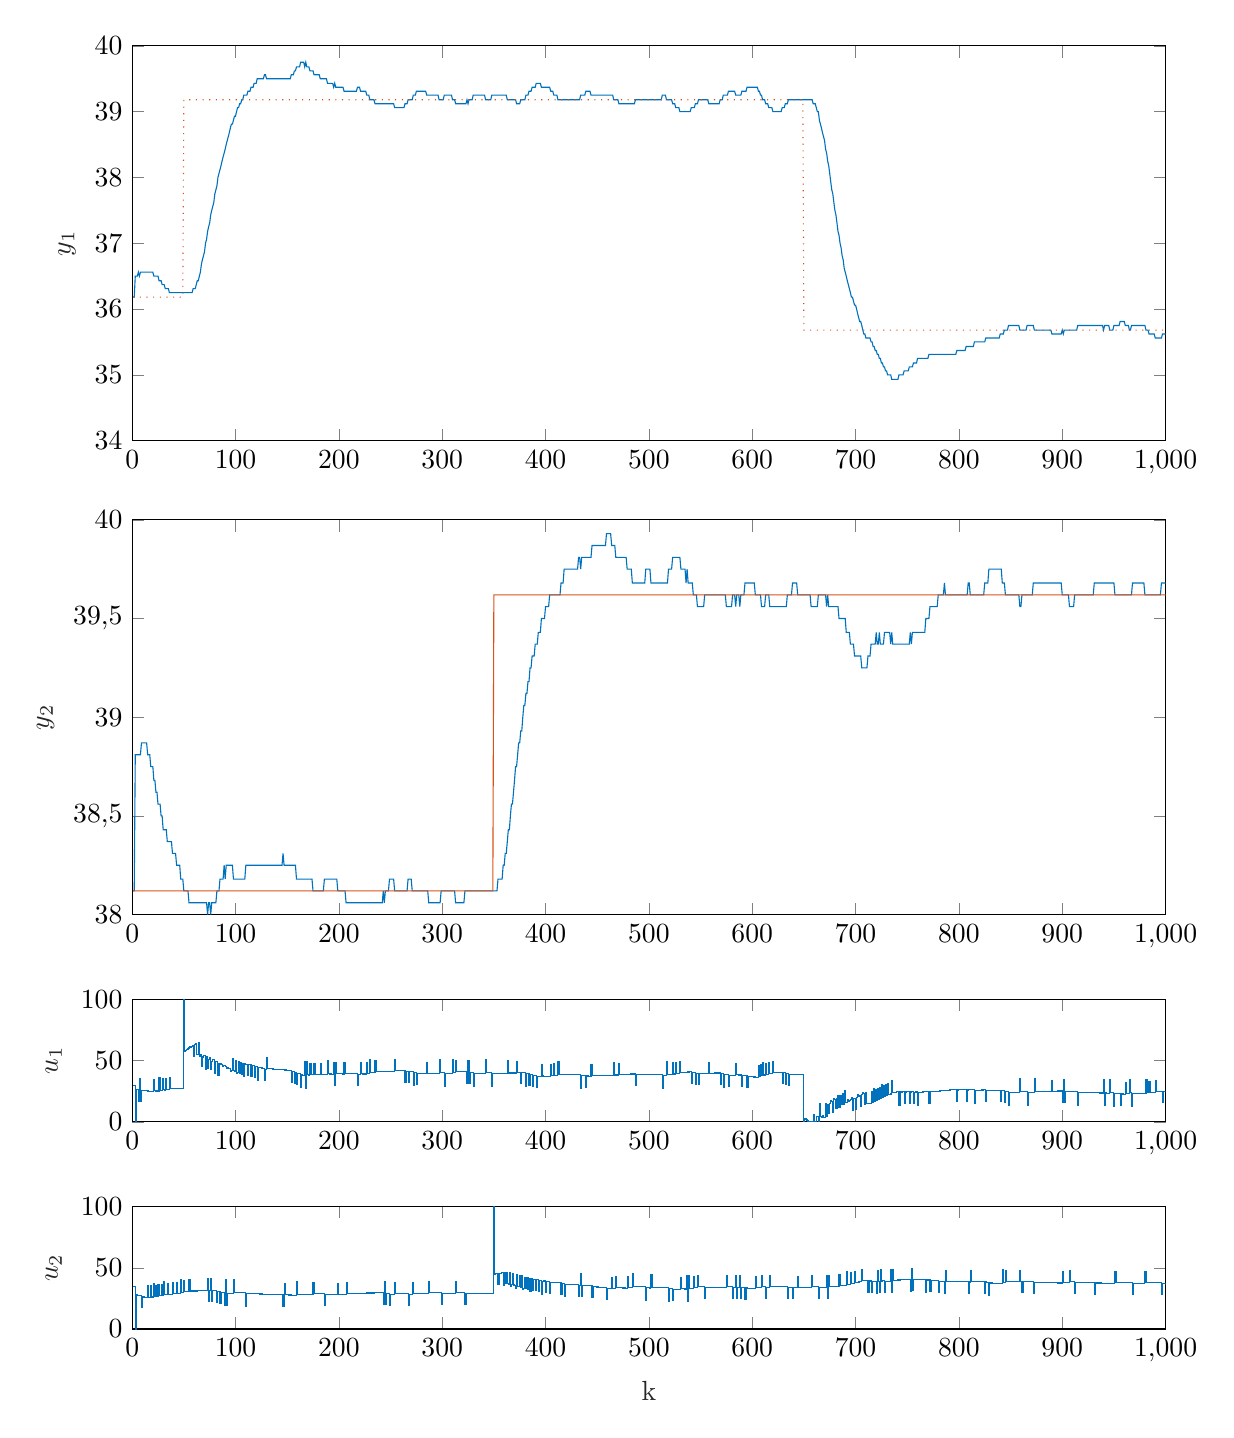
\begin{tikzpicture}

\begin{axis}[%
width=5.167in,
height=0.612in,
at={(0.646in,0.494in)},
scale only axis,
xmin=0,
xmax=1000,
xtick={0,100,200,300,400,500,600,700,800,900,1000},
xlabel style={font=\color{white!15!black}},
xlabel={k},
ymin=0,
ymax=100,
ytick={0,50,100},
ylabel style={font=\color{white!15!black}},
ylabel={$\text{u}_\text{2}$},
axis background/.style={fill=white}
]
\addplot[const plot, color=mycolor1, forget plot] table[row sep=crcr] {%
1	35\\
2	35\\
3	0\\
4	27.87\\
5	27.7167\\
6	27.5633\\
7	27.41\\
8	27.2567\\
9	17.497\\
10	26.33\\
11	26.1633\\
12	25.9967\\
13	25.83\\
14	25.6633\\
15	35.10333\\
16	25.95\\
17	25.7967\\
18	35.25\\
19	26.11\\
20	25.97\\
21	37.0378\\
22	26.4133\\
23	35.89556\\
24	26.7844\\
25	36.28\\
26	27.1822\\
27	27.0844\\
28	36.5933\\
29	27.5089\\
30	38.6322\\
31	28.0633\\
32	27.9944\\
33	27.9256\\
34	37.4633\\
35	28.4078\\
36	28.3522\\
37	28.2967\\
38	28.2411\\
39	37.7922\\
40	28.75\\
41	28.7078\\
42	28.6656\\
43	38.23\\
44	29.2011\\
45	29.1722\\
46	29.1433\\
47	40.3222\\
48	29.8089\\
49	29.7956\\
50	39.3889\\
51	30.3889\\
52	30.3889\\
53	30.3889\\
54	30.3889\\
55	39.9956\\
56	31.0089\\
57	31.0222\\
58	31.0356\\
59	31.0489\\
60	31.0622\\
61	31.0756\\
62	31.0889\\
63	31.1022\\
64	31.1156\\
65	31.1289\\
66	31.1422\\
67	31.1556\\
68	31.1689\\
69	31.1822\\
70	31.1956\\
71	31.2089\\
72	31.2222\\
73	40.8422\\
74	22.262\\
75	31.2756\\
76	40.8956\\
77	22.316\\
78	31.3289\\
79	31.3422\\
80	31.3556\\
81	31.3689\\
82	21.776\\
83	30.7756\\
84	30.7756\\
85	21.169\\
86	30.1556\\
87	30.1422\\
88	30.1289\\
89	18.908\\
90	40.5867\\
91	18.866\\
92	29.3367\\
93	29.3078\\
94	29.2789\\
95	29.25\\
96	29.2211\\
97	29.1922\\
98	40.3711\\
99	29.8578\\
100	29.8444\\
101	29.8311\\
102	29.8178\\
103	29.8044\\
104	29.7911\\
105	29.7778\\
106	29.7644\\
107	29.7511\\
108	29.7378\\
109	29.7244\\
110	18.503\\
111	28.9744\\
112	28.9456\\
113	28.9167\\
114	28.8878\\
115	28.8589\\
116	28.83\\
117	28.8011\\
118	28.7722\\
119	28.7433\\
120	28.7144\\
121	28.6856\\
122	28.6567\\
123	28.6278\\
124	28.5989\\
125	28.57\\
126	28.5411\\
127	28.5122\\
128	28.4833\\
129	28.4544\\
130	28.4256\\
131	28.3967\\
132	28.3678\\
133	28.3389\\
134	28.31\\
135	28.2811\\
136	28.2522\\
137	28.2233\\
138	28.1944\\
139	28.1656\\
140	28.1367\\
141	28.1078\\
142	28.0789\\
143	28.05\\
144	28.0211\\
145	27.9922\\
146	18.357\\
147	36.9211\\
148	27.8922\\
149	27.8633\\
150	27.8344\\
151	27.8056\\
152	27.7767\\
153	27.7478\\
154	27.7189\\
155	27.69\\
156	27.6611\\
157	27.6322\\
158	27.6033\\
159	38.7822\\
160	28.2689\\
161	28.2556\\
162	28.2422\\
163	28.2289\\
164	28.2156\\
165	28.2022\\
166	28.1889\\
167	28.1756\\
168	28.1622\\
169	28.1489\\
170	28.1356\\
171	28.1222\\
172	28.1089\\
173	28.0956\\
174	28.0822\\
175	37.6756\\
176	28.6756\\
177	28.6756\\
178	28.6756\\
179	28.6756\\
180	28.6756\\
181	28.6756\\
182	28.6756\\
183	28.6756\\
184	28.6756\\
185	28.6756\\
186	19.069\\
187	28.0556\\
188	28.0422\\
189	28.0289\\
190	28.0156\\
191	28.0022\\
192	27.9889\\
193	27.9756\\
194	27.9622\\
195	27.9489\\
196	27.9356\\
197	27.9222\\
198	27.9089\\
199	37.5022\\
200	28.5022\\
201	28.5022\\
202	28.5022\\
203	28.5022\\
204	28.5022\\
205	28.5022\\
206	28.5022\\
207	38.1089\\
208	29.1222\\
209	29.1356\\
210	29.1489\\
211	29.1622\\
212	29.1756\\
213	29.1889\\
214	29.2022\\
215	29.2156\\
216	29.2289\\
217	29.2422\\
218	29.2556\\
219	29.2689\\
220	29.2822\\
221	29.2956\\
222	29.3089\\
223	29.3222\\
224	29.3356\\
225	29.3489\\
226	29.3622\\
227	29.3756\\
228	29.3889\\
229	29.4022\\
230	29.4156\\
231	29.4289\\
232	29.4422\\
233	29.4556\\
234	29.4689\\
235	29.4822\\
236	29.4956\\
237	29.5089\\
238	29.5222\\
239	29.5356\\
240	29.5489\\
241	29.5622\\
242	29.5756\\
243	19.982\\
244	38.5889\\
245	19.996\\
246	28.9956\\
247	28.9956\\
248	28.9956\\
249	19.389\\
250	28.3756\\
251	28.3622\\
252	28.3489\\
253	28.3356\\
254	37.9289\\
255	28.9289\\
256	28.9289\\
257	28.9289\\
258	28.9289\\
259	28.9289\\
260	28.9289\\
261	28.9289\\
262	28.9289\\
263	28.9289\\
264	28.9289\\
265	28.9289\\
266	28.9289\\
267	19.322\\
268	28.3089\\
269	28.2956\\
270	28.2822\\
271	37.8756\\
272	28.8756\\
273	28.8756\\
274	28.8756\\
275	28.8756\\
276	28.8756\\
277	28.8756\\
278	28.8756\\
279	28.8756\\
280	28.8756\\
281	28.8756\\
282	28.8756\\
283	28.8756\\
284	28.8756\\
285	28.8756\\
286	28.8756\\
287	38.4822\\
288	29.4956\\
289	29.5089\\
290	29.5222\\
291	29.5356\\
292	29.5489\\
293	29.5622\\
294	29.5756\\
295	29.5889\\
296	29.6022\\
297	29.6156\\
298	29.6289\\
299	20.036\\
300	29.0356\\
301	29.0356\\
302	29.0356\\
303	29.0356\\
304	29.0356\\
305	29.0356\\
306	29.0356\\
307	29.0356\\
308	29.0356\\
309	29.0356\\
310	29.0356\\
311	29.0356\\
312	29.0356\\
313	38.6422\\
314	29.6556\\
315	29.6689\\
316	29.6822\\
317	29.6956\\
318	29.7089\\
319	29.7222\\
320	29.7356\\
321	29.7489\\
322	20.156\\
323	29.1556\\
324	29.1556\\
325	29.1556\\
326	29.1556\\
327	29.1556\\
328	29.1556\\
329	29.1556\\
330	29.1556\\
331	29.1556\\
332	29.1556\\
333	29.1556\\
334	29.1556\\
335	29.1556\\
336	29.1556\\
337	29.1556\\
338	29.1556\\
339	29.1556\\
340	29.1556\\
341	29.1556\\
342	29.1556\\
343	29.1556\\
344	29.1556\\
345	29.1556\\
346	29.1556\\
347	29.1556\\
348	29.1556\\
349	29.1556\\
350	100\\
351	44.6556\\
352	44.9889\\
353	45.322\\
354	36.0489\\
355	45.369\\
356	45.689\\
357	46.009\\
358	46.329\\
359	35.44111\\
360	46.246\\
361	36.9433\\
362	46.234\\
363	36.9189\\
364	36.59\\
365	45.854\\
366	34.911111\\
367	36.0533\\
368	45.289\\
369	35.91778\\
370	35.53333\\
371	33.5344\\
372	44.2278\\
373	34.81444\\
374	34.38778\\
375	43.5544\\
376	34.11444\\
377	43.2678\\
378	32.2133\\
379	33.2444\\
380	42.3689\\
381	32.8867\\
382	41.9978\\
383	32.5022\\
384	41.6\\
385	30.49\\
386	41.0722\\
387	31.5478\\
388	40.6167\\
389	40.6856\\
390	31.1478\\
391	40.2033\\
392	40.2589\\
393	30.7078\\
394	39.75\\
395	39.7922\\
396	28.6267\\
397	39.1533\\
398	39.18\\
399	39.2067\\
400	29.6267\\
401	38.64\\
402	38.6533\\
403	38.6667\\
404	29.0733\\
405	38.0733\\
406	38.0733\\
407	38.0733\\
408	38.0733\\
409	38.0733\\
410	38.0733\\
411	38.0733\\
412	38.0733\\
413	38.0733\\
414	38.0733\\
415	28.4667\\
416	37.4533\\
417	37.44\\
418	26.2189\\
419	36.69\\
420	36.6611\\
421	36.6322\\
422	36.6033\\
423	36.5744\\
424	36.5456\\
425	36.5167\\
426	36.4878\\
427	36.4589\\
428	36.43\\
429	36.4011\\
430	36.3722\\
431	36.3433\\
432	26.7078\\
433	35.66556\\
434	45.23\\
435	26.5944\\
436	35.55222\\
437	35.51\\
438	35.46778\\
439	35.42556\\
440	35.38333\\
441	35.34111\\
442	35.29889\\
443	35.25667\\
444	35.21444\\
445	25.5656\\
446	34.51\\
447	34.45444\\
448	34.39889\\
449	34.34333\\
450	34.28778\\
451	34.23222\\
452	34.17667\\
453	34.12111\\
454	34.06556\\
455	34.01\\
456	33.9544\\
457	33.8989\\
458	33.8433\\
459	24.181\\
460	33.1122\\
461	33.0433\\
462	32.9744\\
463	32.9056\\
464	42.4433\\
465	33.3878\\
466	33.3322\\
467	33.2767\\
468	42.8278\\
469	33.7856\\
470	33.7433\\
471	33.7011\\
472	33.6589\\
473	33.6167\\
474	33.5744\\
475	33.5322\\
476	33.49\\
477	33.4478\\
478	33.4056\\
479	42.97\\
480	33.9411\\
481	33.9122\\
482	33.8833\\
483	33.8544\\
484	45.033\\
485	34.52\\
486	34.50667\\
487	34.49333\\
488	34.48\\
489	34.46667\\
490	34.45333\\
491	34.44\\
492	34.42667\\
493	34.41333\\
494	34.4\\
495	34.38667\\
496	34.37333\\
497	23.152\\
498	33.6233\\
499	33.5944\\
500	33.5656\\
501	33.5367\\
502	44.7156\\
503	34.20222\\
504	34.18889\\
505	34.17556\\
506	34.16222\\
507	34.14889\\
508	34.13556\\
509	34.12222\\
510	34.10889\\
511	34.09556\\
512	34.08222\\
513	34.06889\\
514	34.05556\\
515	34.04222\\
516	34.02889\\
517	34.01556\\
518	34.00222\\
519	22.781\\
520	33.2522\\
521	33.2233\\
522	33.1944\\
523	23.559\\
524	32.5167\\
525	32.4744\\
526	32.4322\\
527	32.39\\
528	32.3478\\
529	32.3056\\
530	32.2633\\
531	41.8278\\
532	32.7989\\
533	32.77\\
534	32.7411\\
535	32.7122\\
536	43.8911\\
537	22.17\\
538	43.8489\\
539	33.3356\\
540	33.3222\\
541	33.3089\\
542	33.2956\\
543	42.8889\\
544	33.8889\\
545	33.8889\\
546	33.8889\\
547	43.4956\\
548	34.50889\\
549	34.52222\\
550	34.53556\\
551	34.54889\\
552	34.56222\\
553	34.57556\\
554	24.982\\
555	33.9822\\
556	33.9822\\
557	33.9822\\
558	33.9822\\
559	33.9822\\
560	33.9822\\
561	33.9822\\
562	33.9822\\
563	33.9822\\
564	33.9822\\
565	33.9822\\
566	33.9822\\
567	33.9822\\
568	33.9822\\
569	33.9822\\
570	33.9822\\
571	33.9822\\
572	33.9822\\
573	33.9822\\
574	33.9822\\
575	43.5889\\
576	34.60222\\
577	34.61556\\
578	34.62889\\
579	34.64222\\
580	34.65556\\
581	25.0622\\
582	34.06222\\
583	34.06222\\
584	43.6689\\
585	25.0756\\
586	34.07556\\
587	34.07556\\
588	43.6822\\
589	25.0889\\
590	34.08889\\
591	34.08889\\
592	34.08889\\
593	24.482\\
594	33.4689\\
595	33.4556\\
596	33.4422\\
597	33.4289\\
598	33.4156\\
599	33.4022\\
600	33.3889\\
601	33.3756\\
602	33.3622\\
603	42.9556\\
604	33.9556\\
605	33.9556\\
606	33.9556\\
607	33.9556\\
608	33.9556\\
609	43.5622\\
610	34.57556\\
611	34.58889\\
612	34.60222\\
613	25.0089\\
614	34.00889\\
615	34.00889\\
616	34.00889\\
617	43.6156\\
618	34.62889\\
619	34.64222\\
620	34.65556\\
621	34.66889\\
622	34.68222\\
623	34.69556\\
624	34.70889\\
625	34.72222\\
626	34.73556\\
627	34.74889\\
628	34.76222\\
629	34.77556\\
630	34.78889\\
631	34.80222\\
632	34.81556\\
633	34.82889\\
634	25.2356\\
635	34.23556\\
636	34.23556\\
637	34.23556\\
638	34.23556\\
639	24.629\\
640	33.6156\\
641	33.6022\\
642	33.5889\\
643	33.5756\\
644	43.1689\\
645	34.16889\\
646	34.16889\\
647	34.16889\\
648	34.16889\\
649	34.16889\\
650	34.16889\\
651	34.16889\\
652	34.16889\\
653	34.16889\\
654	34.16889\\
655	34.16889\\
656	34.16889\\
657	43.7756\\
658	34.78889\\
659	34.80222\\
660	34.81556\\
661	34.82889\\
662	34.84222\\
663	34.85556\\
664	25.2622\\
665	34.26222\\
666	34.26222\\
667	34.26222\\
668	34.26222\\
669	34.26222\\
670	34.26222\\
671	34.26222\\
672	43.8689\\
673	25.2756\\
674	43.8822\\
675	34.89556\\
676	34.908889\\
677	34.922222\\
678	34.935556\\
679	34.948889\\
680	34.962222\\
681	34.975556\\
682	34.988889\\
683	35.0022222\\
684	44.6222\\
685	35.64889\\
686	35.67556\\
687	35.70222\\
688	35.72889\\
689	35.75556\\
690	35.78222\\
691	47.017\\
692	36.5589\\
693	36.6011\\
694	36.6433\\
695	46.292\\
696	37.3478\\
697	37.4033\\
698	37.4589\\
699	47.121\\
700	38.19\\
701	38.2589\\
702	38.3278\\
703	38.3967\\
704	38.4656\\
705	38.5344\\
706	48.21\\
707	39.2922\\
708	39.3744\\
709	39.4567\\
710	39.5389\\
711	39.6211\\
712	30.0967\\
713	39.1656\\
714	39.2344\\
715	29.6967\\
716	38.7522\\
717	38.8078\\
718	38.8633\\
719	38.9189\\
720	29.3678\\
721	48.017\\
722	39.0722\\
723	29.5211\\
724	48.17\\
725	39.2256\\
726	39.2811\\
727	39.3367\\
728	29.7856\\
729	38.8278\\
730	38.87\\
731	38.9122\\
732	38.9544\\
733	38.9967\\
734	48.646\\
735	30.0944\\
736	48.743\\
737	39.7989\\
738	39.8544\\
739	39.91\\
740	39.9656\\
741	40.0211\\
742	40.0767\\
743	40.1322\\
744	40.1878\\
745	40.2433\\
746	40.2989\\
747	40.3544\\
748	40.41\\
749	40.4656\\
750	40.5211\\
751	40.5767\\
752	40.6322\\
753	31.0811\\
754	49.73\\
755	31.1789\\
756	40.2211\\
757	40.2633\\
758	40.3056\\
759	40.3478\\
760	40.39\\
761	40.4322\\
762	40.4744\\
763	40.5167\\
764	40.5589\\
765	40.6011\\
766	40.6433\\
767	40.6856\\
768	29.52\\
769	40.0467\\
770	40.0733\\
771	40.1\\
772	30.52\\
773	39.5333\\
774	39.5467\\
775	39.56\\
776	39.5733\\
777	39.5867\\
778	39.6\\
779	39.6133\\
780	30.02\\
781	39.02\\
782	39.02\\
783	39.02\\
784	39.02\\
785	39.02\\
786	29.4133\\
787	48.007\\
788	39.0067\\
789	39.0067\\
790	39.0067\\
791	39.0067\\
792	39.0067\\
793	39.0067\\
794	39.0067\\
795	39.0067\\
796	39.0067\\
797	39.0067\\
798	39.0067\\
799	39.0067\\
800	39.0067\\
801	39.0067\\
802	39.0067\\
803	39.0067\\
804	39.0067\\
805	39.0067\\
806	39.0067\\
807	39.0067\\
808	39.0067\\
809	29.4\\
810	38.3867\\
811	47.98\\
812	38.98\\
813	38.98\\
814	38.98\\
815	38.98\\
816	38.98\\
817	38.98\\
818	38.98\\
819	38.98\\
820	38.98\\
821	38.98\\
822	38.98\\
823	38.98\\
824	38.98\\
825	29.3733\\
826	38.36\\
827	38.3467\\
828	38.3333\\
829	27.1122\\
830	37.5833\\
831	37.5544\\
832	37.5256\\
833	37.4967\\
834	37.4678\\
835	37.4389\\
836	37.41\\
837	37.3811\\
838	37.3522\\
839	37.3233\\
840	37.2944\\
841	37.2656\\
842	48.444\\
843	37.9311\\
844	37.9178\\
845	47.511\\
846	38.5111\\
847	38.5111\\
848	38.5111\\
849	38.5111\\
850	38.5111\\
851	38.5111\\
852	38.5111\\
853	38.5111\\
854	38.5111\\
855	38.5111\\
856	38.5111\\
857	38.5111\\
858	38.5111\\
859	48.118\\
860	39.1311\\
861	29.5378\\
862	38.5378\\
863	38.5378\\
864	38.5378\\
865	38.5378\\
866	38.5378\\
867	38.5378\\
868	38.5378\\
869	38.5378\\
870	38.5378\\
871	38.5378\\
872	28.9311\\
873	37.9178\\
874	37.9044\\
875	37.8911\\
876	37.8778\\
877	37.8644\\
878	37.8511\\
879	37.8378\\
880	37.8244\\
881	37.8111\\
882	37.7978\\
883	37.7844\\
884	37.7711\\
885	37.7578\\
886	37.7444\\
887	37.7311\\
888	37.7178\\
889	37.7044\\
890	37.6911\\
891	37.6778\\
892	37.6644\\
893	37.6511\\
894	37.6378\\
895	37.6244\\
896	37.6111\\
897	37.5978\\
898	37.5844\\
899	37.5711\\
900	47.164\\
901	38.1644\\
902	38.1644\\
903	38.1644\\
904	38.1644\\
905	38.1644\\
906	38.1644\\
907	47.771\\
908	38.7844\\
909	38.7978\\
910	38.8111\\
911	38.8244\\
912	29.2311\\
913	38.2311\\
914	38.2311\\
915	38.2311\\
916	38.2311\\
917	38.2311\\
918	38.2311\\
919	38.2311\\
920	38.2311\\
921	38.2311\\
922	38.2311\\
923	38.2311\\
924	38.2311\\
925	38.2311\\
926	38.2311\\
927	38.2311\\
928	38.2311\\
929	38.2311\\
930	38.2311\\
931	28.6244\\
932	37.6111\\
933	37.5978\\
934	37.5844\\
935	37.5711\\
936	37.5578\\
937	37.5444\\
938	37.5311\\
939	37.5178\\
940	37.5044\\
941	37.4911\\
942	37.4778\\
943	37.4644\\
944	37.4511\\
945	37.4378\\
946	37.4244\\
947	37.4111\\
948	37.3978\\
949	37.3844\\
950	37.3711\\
951	46.964\\
952	37.9644\\
953	37.9644\\
954	37.9644\\
955	37.9644\\
956	37.9644\\
957	37.9644\\
958	37.9644\\
959	37.9644\\
960	37.9644\\
961	37.9644\\
962	37.9644\\
963	37.9644\\
964	37.9644\\
965	37.9644\\
966	37.9644\\
967	37.9644\\
968	28.3578\\
969	37.3444\\
970	37.3311\\
971	37.3178\\
972	37.3044\\
973	37.2911\\
974	37.2778\\
975	37.2644\\
976	37.2511\\
977	37.2378\\
978	37.2244\\
979	37.2111\\
980	46.804\\
981	37.8044\\
982	37.8044\\
983	37.8044\\
984	37.8044\\
985	37.8044\\
986	37.8044\\
987	37.8044\\
988	37.8044\\
989	37.8044\\
990	37.8044\\
991	37.8044\\
992	37.8044\\
993	37.8044\\
994	37.8044\\
995	37.8044\\
996	28.1978\\
997	37.1844\\
998	37.1711\\
999	37.1578\\
1000	37.1444\\
};
\end{axis}

\begin{axis}[%
width=5.167in,
height=0.612in,
at={(0.646in,1.53in)},
scale only axis,
xmin=0,
xmax=1000,
xtick={0,100,200,300,400,500,600,700,800,900,1000},
ymin=0,
ymax=100,
ytick={0,50,100},
ylabel style={font=\color{white!15!black}},
ylabel={$\text{u}_\text{1}$},
axis background/.style={fill=white}
]
\addplot[const plot, color=mycolor1, forget plot] table[row sep=crcr] {%
1	30\\
2	30\\
3	0\\
4	26.6933\\
5	26.6222\\
6	16.944\\
7	35.4667\\
8	16.789\\
9	25.7044\\
10	25.62\\
11	25.5356\\
12	25.4511\\
13	25.3667\\
14	25.2822\\
15	25.1978\\
16	25.1133\\
17	25.0289\\
18	24.9444\\
19	24.86\\
20	24.7756\\
21	34.2978\\
22	25.2267\\
23	25.1556\\
24	25.0844\\
25	25.0133\\
26	36.15\\
27	25.5944\\
28	25.5389\\
29	35.09\\
30	26.0478\\
31	26.0056\\
32	35.57\\
33	26.5411\\
34	26.5122\\
35	26.4833\\
36	36.0611\\
37	27.0456\\
38	27.03\\
39	27.0144\\
40	26.9989\\
41	26.9833\\
42	26.9678\\
43	26.9522\\
44	26.9367\\
45	26.9211\\
46	26.9056\\
47	26.89\\
48	26.8744\\
49	26.8589\\
50	100\\
51	57.828\\
52	58.479\\
53	59.13\\
54	59.781\\
55	60.432\\
56	61.083\\
57	61.734\\
58	62.386\\
59	53.43\\
60	63.068\\
61	63.706\\
62	54.737\\
63	54.754\\
64	64.366\\
65	53.769\\
66	55.258\\
67	45.627\\
68	52.974\\
69	54.408\\
70	54.328\\
71	43.027\\
72	53.404\\
73	43.662\\
74	50.899\\
75	52.221\\
76	42.423\\
77	49.604\\
78	50.871\\
79	50.624\\
80	39.1567\\
81	49.368\\
82	49.066\\
83	37.5422\\
84	47.698\\
85	47.34\\
86	46.969\\
87	44.983\\
88	46.083\\
89	45.67\\
90	45.243\\
91	43.202\\
92	44.247\\
93	43.778\\
94	43.296\\
95	41.199\\
96	42.188\\
97	51.27\\
98	41.746\\
99	41.208\\
100	50.263\\
101	39.1111\\
102	40.044\\
103	49.071\\
104	39.4911\\
105	48.504\\
106	38.9111\\
107	47.911\\
108	36.7033\\
109	47.188\\
110	47.172\\
111	47.157\\
112	37.5344\\
113	46.506\\
114	46.477\\
115	36.8411\\
116	45.799\\
117	45.757\\
118	36.1078\\
119	45.052\\
120	44.997\\
121	33.7333\\
122	44.162\\
123	44.091\\
124	44.02\\
125	43.949\\
126	43.878\\
127	43.807\\
128	34.1289\\
129	43.044\\
130	52.567\\
131	43.496\\
132	43.424\\
133	43.353\\
134	43.282\\
135	43.211\\
136	43.14\\
137	43.069\\
138	42.998\\
139	42.927\\
140	42.856\\
141	42.784\\
142	42.713\\
143	42.642\\
144	42.571\\
145	42.5\\
146	42.429\\
147	42.358\\
148	42.287\\
149	42.216\\
150	42.144\\
151	42.073\\
152	42.002\\
153	41.931\\
154	32.2533\\
155	41.169\\
156	41.084\\
157	31.3933\\
158	40.296\\
159	30.59111\\
160	39.48\\
161	39.3689\\
162	39.2578\\
163	27.9389\\
164	38.3122\\
165	38.1856\\
166	38.0589\\
167	49.14\\
168	27.3211\\
169	48.902\\
170	38.2911\\
171	38.18\\
172	47.676\\
173	38.5778\\
174	38.48\\
175	38.3822\\
176	47.891\\
177	38.8067\\
178	38.7222\\
179	38.6378\\
180	38.5533\\
181	38.4689\\
182	47.991\\
183	38.92\\
184	38.8489\\
185	38.7778\\
186	38.7067\\
187	38.6356\\
188	38.5644\\
189	49.701\\
190	39.1456\\
191	39.09\\
192	39.0344\\
193	38.9789\\
194	38.9233\\
195	48.474\\
196	29.82556\\
197	48.377\\
198	39.3344\\
199	39.2922\\
200	39.25\\
201	39.2078\\
202	39.1656\\
203	39.1233\\
204	39.0811\\
205	48.646\\
206	39.6167\\
207	39.5878\\
208	39.5589\\
209	39.53\\
210	39.5011\\
211	39.4722\\
212	39.4433\\
213	39.4144\\
214	39.3856\\
215	39.3567\\
216	39.3278\\
217	39.2989\\
218	29.66333\\
219	38.6211\\
220	38.5789\\
221	48.143\\
222	39.1144\\
223	39.0856\\
224	39.0567\\
225	39.0278\\
226	38.9989\\
227	48.577\\
228	39.5611\\
229	39.5456\\
230	50.738\\
231	40.238\\
232	40.238\\
233	40.238\\
234	40.238\\
235	49.844\\
236	40.858\\
237	40.871\\
238	40.884\\
239	40.898\\
240	40.911\\
241	40.924\\
242	40.938\\
243	40.951\\
244	40.964\\
245	40.978\\
246	40.991\\
247	41.004\\
248	41.018\\
249	41.031\\
250	41.044\\
251	41.058\\
252	41.071\\
253	41.084\\
254	50.704\\
255	41.731\\
256	41.758\\
257	41.784\\
258	41.811\\
259	41.838\\
260	41.864\\
261	41.891\\
262	41.918\\
263	41.944\\
264	32.3644\\
265	41.378\\
266	41.391\\
267	31.7978\\
268	40.798\\
269	40.798\\
270	40.798\\
271	40.798\\
272	29.59\\
273	40.074\\
274	40.059\\
275	30.43667\\
276	39.4078\\
277	39.3789\\
278	39.35\\
279	39.3211\\
280	39.2922\\
281	39.2633\\
282	39.2344\\
283	39.2056\\
284	39.1767\\
285	48.754\\
286	39.7389\\
287	39.7233\\
288	39.7078\\
289	39.6922\\
290	39.6767\\
291	39.6611\\
292	39.6456\\
293	39.63\\
294	39.6144\\
295	39.5989\\
296	39.5833\\
297	50.776\\
298	40.276\\
299	40.276\\
300	40.276\\
301	40.276\\
302	29.06778\\
303	39.5522\\
304	39.5367\\
305	39.5211\\
306	39.5056\\
307	39.49\\
308	39.4744\\
309	39.4589\\
310	50.651\\
311	40.151\\
312	40.151\\
313	49.758\\
314	40.771\\
315	40.784\\
316	40.798\\
317	40.811\\
318	40.824\\
319	40.838\\
320	40.851\\
321	40.864\\
322	40.878\\
323	40.891\\
324	31.2978\\
325	49.904\\
326	31.3111\\
327	40.311\\
328	40.311\\
329	40.311\\
330	29.10333\\
331	39.5878\\
332	39.5722\\
333	39.5567\\
334	39.5411\\
335	39.5256\\
336	39.51\\
337	39.4944\\
338	39.4789\\
339	39.4633\\
340	39.4478\\
341	39.4322\\
342	50.624\\
343	40.124\\
344	40.124\\
345	40.124\\
346	40.124\\
347	40.124\\
348	28.9167\\
349	39.4011\\
350	39.3856\\
351	39.37\\
352	39.3544\\
353	39.3389\\
354	39.3233\\
355	39.3078\\
356	39.2922\\
357	39.2767\\
358	39.2611\\
359	39.2456\\
360	39.23\\
361	39.2144\\
362	39.1989\\
363	50.391\\
364	39.8911\\
365	39.8911\\
366	39.8911\\
367	39.8911\\
368	39.8911\\
369	39.8911\\
370	39.8911\\
371	39.8911\\
372	49.498\\
373	40.511\\
374	40.524\\
375	40.538\\
376	30.94444\\
377	39.9444\\
378	39.9444\\
379	39.9444\\
380	39.9444\\
381	28.7367\\
382	39.2211\\
383	39.2056\\
384	29.58333\\
385	38.5544\\
386	38.5256\\
387	28.89\\
388	37.8478\\
389	37.8056\\
390	37.7633\\
391	28.1144\\
392	37.0589\\
393	37.0033\\
394	36.9478\\
395	36.8922\\
396	46.443\\
397	37.4011\\
398	37.3589\\
399	37.3167\\
400	37.2744\\
401	37.2322\\
402	37.19\\
403	37.1478\\
404	37.1056\\
405	46.67\\
406	37.6411\\
407	37.6122\\
408	47.19\\
409	38.1744\\
410	38.1589\\
411	38.1433\\
412	49.336\\
413	38.8356\\
414	38.8356\\
415	38.8356\\
416	38.8356\\
417	38.8356\\
418	38.8356\\
419	38.8356\\
420	38.8356\\
421	38.8356\\
422	38.8356\\
423	38.8356\\
424	38.8356\\
425	38.8356\\
426	38.8356\\
427	38.8356\\
428	38.8356\\
429	38.8356\\
430	38.8356\\
431	38.8356\\
432	38.8356\\
433	38.8356\\
434	27.6278\\
435	38.1122\\
436	38.0967\\
437	38.0811\\
438	38.0656\\
439	28.4433\\
440	37.4144\\
441	37.3856\\
442	37.3567\\
443	37.3278\\
444	46.906\\
445	37.89\\
446	37.8744\\
447	37.8589\\
448	37.8433\\
449	37.8278\\
450	37.8122\\
451	37.7967\\
452	37.7811\\
453	37.7656\\
454	37.75\\
455	37.7344\\
456	37.7189\\
457	37.7033\\
458	37.6878\\
459	37.6722\\
460	37.6567\\
461	37.6411\\
462	37.6256\\
463	37.61\\
464	37.5944\\
465	37.5789\\
466	48.771\\
467	38.2711\\
468	38.2711\\
469	38.2711\\
470	38.2711\\
471	47.878\\
472	38.8911\\
473	38.9044\\
474	38.9178\\
475	38.9311\\
476	38.9444\\
477	38.9578\\
478	38.9711\\
479	38.9844\\
480	38.9978\\
481	39.0111\\
482	39.0244\\
483	39.0378\\
484	39.0511\\
485	39.0644\\
486	39.0778\\
487	29.48444\\
488	38.4844\\
489	38.4844\\
490	38.4844\\
491	38.4844\\
492	38.4844\\
493	38.4844\\
494	38.4844\\
495	38.4844\\
496	38.4844\\
497	38.4844\\
498	38.4844\\
499	38.4844\\
500	38.4844\\
501	38.4844\\
502	38.4844\\
503	38.4844\\
504	38.4844\\
505	38.4844\\
506	38.4844\\
507	38.4844\\
508	38.4844\\
509	38.4844\\
510	38.4844\\
511	38.4844\\
512	38.4844\\
513	27.2767\\
514	37.7611\\
515	37.7456\\
516	37.73\\
517	48.922\\
518	38.4222\\
519	38.4222\\
520	38.4222\\
521	38.4222\\
522	38.4222\\
523	48.029\\
524	39.0422\\
525	39.0556\\
526	48.676\\
527	39.7022\\
528	39.7289\\
529	39.7556\\
530	49.389\\
531	40.429\\
532	40.469\\
533	40.509\\
534	40.549\\
535	40.589\\
536	40.629\\
537	40.669\\
538	40.709\\
539	40.749\\
540	40.789\\
541	31.2222\\
542	40.249\\
543	40.276\\
544	40.302\\
545	30.72222\\
546	39.7356\\
547	39.7489\\
548	30.15556\\
549	39.1556\\
550	39.1556\\
551	39.1556\\
552	39.1556\\
553	39.1556\\
554	39.1556\\
555	39.1556\\
556	39.1556\\
557	39.1556\\
558	48.762\\
559	39.7756\\
560	39.7889\\
561	39.8022\\
562	39.8156\\
563	39.8289\\
564	39.8422\\
565	39.8556\\
566	39.8689\\
567	39.8822\\
568	39.8956\\
569	30.30222\\
570	39.3022\\
571	39.3022\\
572	28.0944\\
573	38.5789\\
574	38.5633\\
575	38.5478\\
576	38.5322\\
577	28.91\\
578	37.8811\\
579	37.8522\\
580	37.8233\\
581	37.7944\\
582	37.7656\\
583	37.7367\\
584	47.314\\
585	38.2989\\
586	38.2833\\
587	38.2678\\
588	38.2522\\
589	38.2367\\
590	28.6144\\
591	37.5856\\
592	37.5567\\
593	37.5278\\
594	37.4989\\
595	27.8633\\
596	36.8211\\
597	36.7789\\
598	36.7367\\
599	36.6944\\
600	36.6522\\
601	36.61\\
602	36.5678\\
603	36.5256\\
604	36.4833\\
605	36.4411\\
606	46.006\\
607	36.9767\\
608	46.554\\
609	37.5389\\
610	48.731\\
611	38.2311\\
612	38.2311\\
613	47.838\\
614	38.8511\\
615	38.8644\\
616	48.484\\
617	39.5111\\
618	39.5378\\
619	39.5644\\
620	49.198\\
621	40.238\\
622	40.278\\
623	40.318\\
624	40.358\\
625	40.398\\
626	40.438\\
627	40.478\\
628	40.518\\
629	30.95111\\
630	39.9778\\
631	40.004\\
632	30.42444\\
633	39.4378\\
634	39.4511\\
635	29.85778\\
636	38.8578\\
637	38.8578\\
638	38.8578\\
639	38.8578\\
640	38.8578\\
641	38.8578\\
642	38.8578\\
643	38.8578\\
644	38.8578\\
645	38.8578\\
646	38.8578\\
647	38.8578\\
648	38.8578\\
649	38.8578\\
650	0\\
651	2.691\\
652	1.913\\
653	1.136\\
654	0.358000000000001\\
655	0\\
656	0\\
657	0\\
658	0\\
659	6.076\\
660	0\\
661	0\\
662	4.389\\
663	4.244\\
664	0\\
665	14.583\\
666	3.981\\
667	3.892\\
668	5.418\\
669	3.858\\
670	3.811\\
671	14.986\\
672	4.481\\
673	14.097\\
674	6.733\\
675	14.891\\
676	17.177\\
677	16.39\\
678	7.523\\
679	18.878\\
680	18.16\\
681	10.963\\
682	19.288\\
683	21.74\\
684	11.513\\
685	21.4067\\
686	14.321\\
687	22.7567\\
688	14.112\\
689	25.6889\\
690	15.587\\
691	15.998\\
692	18.023\\
693	16.963\\
694	17.417\\
695	17.883\\
696	19.964\\
697	9.353\\
698	18.849\\
699	19.358\\
700	10.273\\
701	19.796\\
702	21.9322\\
703	20.9833\\
704	21.5478\\
705	12.519\\
706	22.0967\\
707	24.2889\\
708	23.3956\\
709	14.409\\
710	24.0289\\
711	15.056\\
712	15.082\\
713	15.109\\
714	15.136\\
715	24.7689\\
716	15.809\\
717	27.0567\\
718	16.612\\
719	26.2744\\
720	17.343\\
721	27.0189\\
722	18.101\\
723	27.79\\
724	18.886\\
725	30.18889\\
726	19.8\\
727	29.51778\\
728	20.6422\\
729	30.37333\\
730	21.5111\\
731	31.2556\\
732	22.4067\\
733	22.5578\\
734	22.7089\\
735	34.0678\\
736	23.7344\\
737	23.9011\\
738	24.0678\\
739	24.2344\\
740	24.4011\\
741	24.5678\\
742	13.527\\
743	24.1778\\
744	24.3289\\
745	24.48\\
746	24.6311\\
747	15.176\\
748	24.3133\\
749	24.4511\\
750	24.5889\\
751	24.7267\\
752	15.258\\
753	24.3822\\
754	24.5067\\
755	24.6311\\
756	15.149\\
757	24.26\\
758	24.3711\\
759	24.4822\\
760	13.386\\
761	23.9811\\
762	24.0767\\
763	24.1722\\
764	24.2678\\
765	24.3633\\
766	24.4589\\
767	24.5544\\
768	24.65\\
769	24.7456\\
770	24.8411\\
771	15.33\\
772	24.4122\\
773	24.4944\\
774	24.5767\\
775	24.6589\\
776	24.7411\\
777	24.8233\\
778	24.9056\\
779	24.9878\\
780	25.07\\
781	25.1522\\
782	25.2344\\
783	25.3167\\
784	25.3989\\
785	25.4811\\
786	25.5633\\
787	25.6456\\
788	25.7278\\
789	25.81\\
790	25.8922\\
791	25.9744\\
792	26.0567\\
793	26.1389\\
794	26.2211\\
795	26.3033\\
796	26.3856\\
797	26.4678\\
798	16.943\\
799	26.0122\\
800	26.0811\\
801	26.15\\
802	26.2189\\
803	26.2878\\
804	26.3567\\
805	26.4256\\
806	26.4944\\
807	16.957\\
808	26.0122\\
809	26.0678\\
810	26.1233\\
811	26.1789\\
812	26.2344\\
813	26.29\\
814	26.3456\\
815	15.193\\
816	25.7333\\
817	25.7733\\
818	25.8133\\
819	25.8533\\
820	25.8933\\
821	25.9333\\
822	25.9733\\
823	26.0133\\
824	26.0533\\
825	26.0933\\
826	16.527\\
827	25.5533\\
828	25.58\\
829	25.6067\\
830	25.6333\\
831	25.66\\
832	25.6867\\
833	25.7133\\
834	25.74\\
835	25.7667\\
836	25.7933\\
837	25.82\\
838	25.8467\\
839	25.8733\\
840	16.293\\
841	25.3067\\
842	25.32\\
843	25.3333\\
844	15.74\\
845	24.74\\
846	24.74\\
847	24.74\\
848	13.532\\
849	24.0167\\
850	24.0011\\
851	23.9856\\
852	23.97\\
853	23.9544\\
854	23.9389\\
855	23.9233\\
856	23.9078\\
857	23.8922\\
858	23.8767\\
859	35.0689\\
860	24.5689\\
861	24.5689\\
862	24.5689\\
863	24.5689\\
864	24.5689\\
865	24.5689\\
866	13.361\\
867	23.8456\\
868	23.83\\
869	23.8144\\
870	23.7989\\
871	23.7833\\
872	23.7678\\
873	34.96\\
874	24.46\\
875	24.46\\
876	24.46\\
877	24.46\\
878	24.46\\
879	24.46\\
880	24.46\\
881	24.46\\
882	24.46\\
883	24.46\\
884	24.46\\
885	24.46\\
886	24.46\\
887	24.46\\
888	24.46\\
889	24.46\\
890	34.0667\\
891	25.08\\
892	25.0933\\
893	25.1067\\
894	25.12\\
895	25.1333\\
896	25.1467\\
897	25.16\\
898	25.1733\\
899	25.1867\\
900	15.593\\
901	34.2\\
902	15.607\\
903	24.6067\\
904	24.6067\\
905	24.6067\\
906	24.6067\\
907	24.6067\\
908	24.6067\\
909	24.6067\\
910	24.6067\\
911	24.6067\\
912	24.6067\\
913	24.6067\\
914	24.6067\\
915	13.399\\
916	23.8833\\
917	23.8678\\
918	23.8522\\
919	23.8367\\
920	23.8211\\
921	23.8056\\
922	23.79\\
923	23.7744\\
924	23.7589\\
925	23.7433\\
926	23.7278\\
927	23.7122\\
928	23.6967\\
929	23.6811\\
930	23.6656\\
931	23.65\\
932	23.6344\\
933	23.6189\\
934	23.6033\\
935	23.5878\\
936	23.5722\\
937	23.5567\\
938	23.5411\\
939	23.5256\\
940	34.7178\\
941	13.01\\
942	23.4944\\
943	23.4789\\
944	23.4633\\
945	23.4478\\
946	34.64\\
947	24.14\\
948	24.14\\
949	24.14\\
950	12.932\\
951	23.4167\\
952	23.4011\\
953	23.3856\\
954	23.37\\
955	23.3544\\
956	13.732\\
957	22.7033\\
958	22.6744\\
959	22.6456\\
960	22.6167\\
961	32.1944\\
962	23.1789\\
963	23.1633\\
964	23.1478\\
965	34.34\\
966	23.84\\
967	12.632\\
968	23.1167\\
969	23.1011\\
970	23.0856\\
971	23.07\\
972	23.0544\\
973	23.0389\\
974	23.0233\\
975	23.0078\\
976	22.9922\\
977	22.9767\\
978	22.9611\\
979	22.9456\\
980	22.93\\
981	34.1222\\
982	23.6222\\
983	23.6222\\
984	33.2289\\
985	24.2422\\
986	24.2556\\
987	24.2689\\
988	24.2822\\
989	24.2956\\
990	33.9156\\
991	24.9422\\
992	24.9689\\
993	24.9956\\
994	25.0222\\
995	25.0489\\
996	25.0756\\
997	15.496\\
998	24.5089\\
999	24.5222\\
1000	24.5356\\
};
\end{axis}

\begin{axis}[%
width=5.167in,
height=1.974in,
at={(0.646in,2.566in)},
scale only axis,
xmin=0,
xmax=1000,
xtick={0,100,200,300,400,500,600,700,800,900,1000},
ymin=38,
ymax=40,
ytick={38,38.5,39,39.5,40},
yticklabels={{38},{38,5},{39},{39,5},{40}},
ylabel style={font=\color{white!15!black}},
ylabel={$\text{y}_\text{2}$},
axis background/.style={fill=white}
]
\addplot [color=mycolor1, forget plot]
  table[row sep=crcr]{%
1	38.12\\
2	38.12\\
3	38.81\\
4	38.81\\
5	38.81\\
6	38.81\\
7	38.81\\
8	38.81\\
9	38.87\\
10	38.87\\
11	38.87\\
12	38.87\\
13	38.87\\
14	38.87\\
15	38.81\\
16	38.81\\
17	38.81\\
18	38.75\\
19	38.75\\
20	38.75\\
21	38.68\\
22	38.68\\
23	38.62\\
24	38.62\\
25	38.56\\
26	38.56\\
27	38.56\\
28	38.5\\
29	38.5\\
30	38.43\\
31	38.43\\
32	38.43\\
33	38.43\\
34	38.37\\
35	38.37\\
36	38.37\\
37	38.37\\
38	38.37\\
39	38.31\\
40	38.31\\
41	38.31\\
42	38.31\\
43	38.25\\
44	38.25\\
45	38.25\\
46	38.25\\
47	38.18\\
48	38.18\\
49	38.18\\
50	38.12\\
51	38.12\\
52	38.12\\
53	38.12\\
54	38.12\\
55	38.06\\
56	38.06\\
57	38.06\\
58	38.06\\
59	38.06\\
60	38.06\\
61	38.06\\
62	38.06\\
63	38.06\\
64	38.06\\
65	38.06\\
66	38.06\\
67	38.06\\
68	38.06\\
69	38.06\\
70	38.06\\
71	38.06\\
72	38.06\\
73	38\\
74	38.06\\
75	38.06\\
76	38\\
77	38.06\\
78	38.06\\
79	38.06\\
80	38.06\\
81	38.06\\
82	38.12\\
83	38.12\\
84	38.12\\
85	38.18\\
86	38.18\\
87	38.18\\
88	38.18\\
89	38.25\\
90	38.18\\
91	38.25\\
92	38.25\\
93	38.25\\
94	38.25\\
95	38.25\\
96	38.25\\
97	38.25\\
98	38.18\\
99	38.18\\
100	38.18\\
101	38.18\\
102	38.18\\
103	38.18\\
104	38.18\\
105	38.18\\
106	38.18\\
107	38.18\\
108	38.18\\
109	38.18\\
110	38.25\\
111	38.25\\
112	38.25\\
113	38.25\\
114	38.25\\
115	38.25\\
116	38.25\\
117	38.25\\
118	38.25\\
119	38.25\\
120	38.25\\
121	38.25\\
122	38.25\\
123	38.25\\
124	38.25\\
125	38.25\\
126	38.25\\
127	38.25\\
128	38.25\\
129	38.25\\
130	38.25\\
131	38.25\\
132	38.25\\
133	38.25\\
134	38.25\\
135	38.25\\
136	38.25\\
137	38.25\\
138	38.25\\
139	38.25\\
140	38.25\\
141	38.25\\
142	38.25\\
143	38.25\\
144	38.25\\
145	38.25\\
146	38.31\\
147	38.25\\
148	38.25\\
149	38.25\\
150	38.25\\
151	38.25\\
152	38.25\\
153	38.25\\
154	38.25\\
155	38.25\\
156	38.25\\
157	38.25\\
158	38.25\\
159	38.18\\
160	38.18\\
161	38.18\\
162	38.18\\
163	38.18\\
164	38.18\\
165	38.18\\
166	38.18\\
167	38.18\\
168	38.18\\
169	38.18\\
170	38.18\\
171	38.18\\
172	38.18\\
173	38.18\\
174	38.18\\
175	38.12\\
176	38.12\\
177	38.12\\
178	38.12\\
179	38.12\\
180	38.12\\
181	38.12\\
182	38.12\\
183	38.12\\
184	38.12\\
185	38.12\\
186	38.18\\
187	38.18\\
188	38.18\\
189	38.18\\
190	38.18\\
191	38.18\\
192	38.18\\
193	38.18\\
194	38.18\\
195	38.18\\
196	38.18\\
197	38.18\\
198	38.18\\
199	38.12\\
200	38.12\\
201	38.12\\
202	38.12\\
203	38.12\\
204	38.12\\
205	38.12\\
206	38.12\\
207	38.06\\
208	38.06\\
209	38.06\\
210	38.06\\
211	38.06\\
212	38.06\\
213	38.06\\
214	38.06\\
215	38.06\\
216	38.06\\
217	38.06\\
218	38.06\\
219	38.06\\
220	38.06\\
221	38.06\\
222	38.06\\
223	38.06\\
224	38.06\\
225	38.06\\
226	38.06\\
227	38.06\\
228	38.06\\
229	38.06\\
230	38.06\\
231	38.06\\
232	38.06\\
233	38.06\\
234	38.06\\
235	38.06\\
236	38.06\\
237	38.06\\
238	38.06\\
239	38.06\\
240	38.06\\
241	38.06\\
242	38.06\\
243	38.12\\
244	38.06\\
245	38.12\\
246	38.12\\
247	38.12\\
248	38.12\\
249	38.18\\
250	38.18\\
251	38.18\\
252	38.18\\
253	38.18\\
254	38.12\\
255	38.12\\
256	38.12\\
257	38.12\\
258	38.12\\
259	38.12\\
260	38.12\\
261	38.12\\
262	38.12\\
263	38.12\\
264	38.12\\
265	38.12\\
266	38.12\\
267	38.18\\
268	38.18\\
269	38.18\\
270	38.18\\
271	38.12\\
272	38.12\\
273	38.12\\
274	38.12\\
275	38.12\\
276	38.12\\
277	38.12\\
278	38.12\\
279	38.12\\
280	38.12\\
281	38.12\\
282	38.12\\
283	38.12\\
284	38.12\\
285	38.12\\
286	38.12\\
287	38.06\\
288	38.06\\
289	38.06\\
290	38.06\\
291	38.06\\
292	38.06\\
293	38.06\\
294	38.06\\
295	38.06\\
296	38.06\\
297	38.06\\
298	38.06\\
299	38.12\\
300	38.12\\
301	38.12\\
302	38.12\\
303	38.12\\
304	38.12\\
305	38.12\\
306	38.12\\
307	38.12\\
308	38.12\\
309	38.12\\
310	38.12\\
311	38.12\\
312	38.12\\
313	38.06\\
314	38.06\\
315	38.06\\
316	38.06\\
317	38.06\\
318	38.06\\
319	38.06\\
320	38.06\\
321	38.06\\
322	38.12\\
323	38.12\\
324	38.12\\
325	38.12\\
326	38.12\\
327	38.12\\
328	38.12\\
329	38.12\\
330	38.12\\
331	38.12\\
332	38.12\\
333	38.12\\
334	38.12\\
335	38.12\\
336	38.12\\
337	38.12\\
338	38.12\\
339	38.12\\
340	38.12\\
341	38.12\\
342	38.12\\
343	38.12\\
344	38.12\\
345	38.12\\
346	38.12\\
347	38.12\\
348	38.12\\
349	38.12\\
350	38.12\\
351	38.12\\
352	38.12\\
353	38.12\\
354	38.18\\
355	38.18\\
356	38.18\\
357	38.18\\
358	38.18\\
359	38.25\\
360	38.25\\
361	38.31\\
362	38.31\\
363	38.37\\
364	38.43\\
365	38.43\\
366	38.5\\
367	38.56\\
368	38.56\\
369	38.62\\
370	38.68\\
371	38.75\\
372	38.75\\
373	38.81\\
374	38.87\\
375	38.87\\
376	38.93\\
377	38.93\\
378	39\\
379	39.06\\
380	39.06\\
381	39.12\\
382	39.12\\
383	39.18\\
384	39.18\\
385	39.25\\
386	39.25\\
387	39.31\\
388	39.31\\
389	39.31\\
390	39.37\\
391	39.37\\
392	39.37\\
393	39.43\\
394	39.43\\
395	39.43\\
396	39.5\\
397	39.5\\
398	39.5\\
399	39.5\\
400	39.56\\
401	39.56\\
402	39.56\\
403	39.56\\
404	39.62\\
405	39.62\\
406	39.62\\
407	39.62\\
408	39.62\\
409	39.62\\
410	39.62\\
411	39.62\\
412	39.62\\
413	39.62\\
414	39.62\\
415	39.68\\
416	39.68\\
417	39.68\\
418	39.75\\
419	39.75\\
420	39.75\\
421	39.75\\
422	39.75\\
423	39.75\\
424	39.75\\
425	39.75\\
426	39.75\\
427	39.75\\
428	39.75\\
429	39.75\\
430	39.75\\
431	39.75\\
432	39.81\\
433	39.81\\
434	39.75\\
435	39.81\\
436	39.81\\
437	39.81\\
438	39.81\\
439	39.81\\
440	39.81\\
441	39.81\\
442	39.81\\
443	39.81\\
444	39.81\\
445	39.87\\
446	39.87\\
447	39.87\\
448	39.87\\
449	39.87\\
450	39.87\\
451	39.87\\
452	39.87\\
453	39.87\\
454	39.87\\
455	39.87\\
456	39.87\\
457	39.87\\
458	39.87\\
459	39.93\\
460	39.93\\
461	39.93\\
462	39.93\\
463	39.93\\
464	39.87\\
465	39.87\\
466	39.87\\
467	39.87\\
468	39.81\\
469	39.81\\
470	39.81\\
471	39.81\\
472	39.81\\
473	39.81\\
474	39.81\\
475	39.81\\
476	39.81\\
477	39.81\\
478	39.81\\
479	39.75\\
480	39.75\\
481	39.75\\
482	39.75\\
483	39.75\\
484	39.68\\
485	39.68\\
486	39.68\\
487	39.68\\
488	39.68\\
489	39.68\\
490	39.68\\
491	39.68\\
492	39.68\\
493	39.68\\
494	39.68\\
495	39.68\\
496	39.68\\
497	39.75\\
498	39.75\\
499	39.75\\
500	39.75\\
501	39.75\\
502	39.68\\
503	39.68\\
504	39.68\\
505	39.68\\
506	39.68\\
507	39.68\\
508	39.68\\
509	39.68\\
510	39.68\\
511	39.68\\
512	39.68\\
513	39.68\\
514	39.68\\
515	39.68\\
516	39.68\\
517	39.68\\
518	39.68\\
519	39.75\\
520	39.75\\
521	39.75\\
522	39.75\\
523	39.81\\
524	39.81\\
525	39.81\\
526	39.81\\
527	39.81\\
528	39.81\\
529	39.81\\
530	39.81\\
531	39.75\\
532	39.75\\
533	39.75\\
534	39.75\\
535	39.75\\
536	39.68\\
537	39.75\\
538	39.68\\
539	39.68\\
540	39.68\\
541	39.68\\
542	39.68\\
543	39.62\\
544	39.62\\
545	39.62\\
546	39.62\\
547	39.56\\
548	39.56\\
549	39.56\\
550	39.56\\
551	39.56\\
552	39.56\\
553	39.56\\
554	39.62\\
555	39.62\\
556	39.62\\
557	39.62\\
558	39.62\\
559	39.62\\
560	39.62\\
561	39.62\\
562	39.62\\
563	39.62\\
564	39.62\\
565	39.62\\
566	39.62\\
567	39.62\\
568	39.62\\
569	39.62\\
570	39.62\\
571	39.62\\
572	39.62\\
573	39.62\\
574	39.62\\
575	39.56\\
576	39.56\\
577	39.56\\
578	39.56\\
579	39.56\\
580	39.56\\
581	39.62\\
582	39.62\\
583	39.62\\
584	39.56\\
585	39.62\\
586	39.62\\
587	39.62\\
588	39.56\\
589	39.62\\
590	39.62\\
591	39.62\\
592	39.62\\
593	39.68\\
594	39.68\\
595	39.68\\
596	39.68\\
597	39.68\\
598	39.68\\
599	39.68\\
600	39.68\\
601	39.68\\
602	39.68\\
603	39.62\\
604	39.62\\
605	39.62\\
606	39.62\\
607	39.62\\
608	39.62\\
609	39.56\\
610	39.56\\
611	39.56\\
612	39.56\\
613	39.62\\
614	39.62\\
615	39.62\\
616	39.62\\
617	39.56\\
618	39.56\\
619	39.56\\
620	39.56\\
621	39.56\\
622	39.56\\
623	39.56\\
624	39.56\\
625	39.56\\
626	39.56\\
627	39.56\\
628	39.56\\
629	39.56\\
630	39.56\\
631	39.56\\
632	39.56\\
633	39.56\\
634	39.62\\
635	39.62\\
636	39.62\\
637	39.62\\
638	39.62\\
639	39.68\\
640	39.68\\
641	39.68\\
642	39.68\\
643	39.68\\
644	39.62\\
645	39.62\\
646	39.62\\
647	39.62\\
648	39.62\\
649	39.62\\
650	39.62\\
651	39.62\\
652	39.62\\
653	39.62\\
654	39.62\\
655	39.62\\
656	39.62\\
657	39.56\\
658	39.56\\
659	39.56\\
660	39.56\\
661	39.56\\
662	39.56\\
663	39.56\\
664	39.62\\
665	39.62\\
666	39.62\\
667	39.62\\
668	39.62\\
669	39.62\\
670	39.62\\
671	39.62\\
672	39.56\\
673	39.62\\
674	39.56\\
675	39.56\\
676	39.56\\
677	39.56\\
678	39.56\\
679	39.56\\
680	39.56\\
681	39.56\\
682	39.56\\
683	39.56\\
684	39.5\\
685	39.5\\
686	39.5\\
687	39.5\\
688	39.5\\
689	39.5\\
690	39.5\\
691	39.43\\
692	39.43\\
693	39.43\\
694	39.43\\
695	39.37\\
696	39.37\\
697	39.37\\
698	39.37\\
699	39.31\\
700	39.31\\
701	39.31\\
702	39.31\\
703	39.31\\
704	39.31\\
705	39.31\\
706	39.25\\
707	39.25\\
708	39.25\\
709	39.25\\
710	39.25\\
711	39.25\\
712	39.31\\
713	39.31\\
714	39.31\\
715	39.37\\
716	39.37\\
717	39.37\\
718	39.37\\
719	39.37\\
720	39.43\\
721	39.37\\
722	39.37\\
723	39.43\\
724	39.37\\
725	39.37\\
726	39.37\\
727	39.37\\
728	39.43\\
729	39.43\\
730	39.43\\
731	39.43\\
732	39.43\\
733	39.43\\
734	39.37\\
735	39.43\\
736	39.37\\
737	39.37\\
738	39.37\\
739	39.37\\
740	39.37\\
741	39.37\\
742	39.37\\
743	39.37\\
744	39.37\\
745	39.37\\
746	39.37\\
747	39.37\\
748	39.37\\
749	39.37\\
750	39.37\\
751	39.37\\
752	39.37\\
753	39.43\\
754	39.37\\
755	39.43\\
756	39.43\\
757	39.43\\
758	39.43\\
759	39.43\\
760	39.43\\
761	39.43\\
762	39.43\\
763	39.43\\
764	39.43\\
765	39.43\\
766	39.43\\
767	39.43\\
768	39.5\\
769	39.5\\
770	39.5\\
771	39.5\\
772	39.56\\
773	39.56\\
774	39.56\\
775	39.56\\
776	39.56\\
777	39.56\\
778	39.56\\
779	39.56\\
780	39.62\\
781	39.62\\
782	39.62\\
783	39.62\\
784	39.62\\
785	39.62\\
786	39.68\\
787	39.62\\
788	39.62\\
789	39.62\\
790	39.62\\
791	39.62\\
792	39.62\\
793	39.62\\
794	39.62\\
795	39.62\\
796	39.62\\
797	39.62\\
798	39.62\\
799	39.62\\
800	39.62\\
801	39.62\\
802	39.62\\
803	39.62\\
804	39.62\\
805	39.62\\
806	39.62\\
807	39.62\\
808	39.62\\
809	39.68\\
810	39.68\\
811	39.62\\
812	39.62\\
813	39.62\\
814	39.62\\
815	39.62\\
816	39.62\\
817	39.62\\
818	39.62\\
819	39.62\\
820	39.62\\
821	39.62\\
822	39.62\\
823	39.62\\
824	39.62\\
825	39.68\\
826	39.68\\
827	39.68\\
828	39.68\\
829	39.75\\
830	39.75\\
831	39.75\\
832	39.75\\
833	39.75\\
834	39.75\\
835	39.75\\
836	39.75\\
837	39.75\\
838	39.75\\
839	39.75\\
840	39.75\\
841	39.75\\
842	39.68\\
843	39.68\\
844	39.68\\
845	39.62\\
846	39.62\\
847	39.62\\
848	39.62\\
849	39.62\\
850	39.62\\
851	39.62\\
852	39.62\\
853	39.62\\
854	39.62\\
855	39.62\\
856	39.62\\
857	39.62\\
858	39.62\\
859	39.56\\
860	39.56\\
861	39.62\\
862	39.62\\
863	39.62\\
864	39.62\\
865	39.62\\
866	39.62\\
867	39.62\\
868	39.62\\
869	39.62\\
870	39.62\\
871	39.62\\
872	39.68\\
873	39.68\\
874	39.68\\
875	39.68\\
876	39.68\\
877	39.68\\
878	39.68\\
879	39.68\\
880	39.68\\
881	39.68\\
882	39.68\\
883	39.68\\
884	39.68\\
885	39.68\\
886	39.68\\
887	39.68\\
888	39.68\\
889	39.68\\
890	39.68\\
891	39.68\\
892	39.68\\
893	39.68\\
894	39.68\\
895	39.68\\
896	39.68\\
897	39.68\\
898	39.68\\
899	39.68\\
900	39.62\\
901	39.62\\
902	39.62\\
903	39.62\\
904	39.62\\
905	39.62\\
906	39.62\\
907	39.56\\
908	39.56\\
909	39.56\\
910	39.56\\
911	39.56\\
912	39.62\\
913	39.62\\
914	39.62\\
915	39.62\\
916	39.62\\
917	39.62\\
918	39.62\\
919	39.62\\
920	39.62\\
921	39.62\\
922	39.62\\
923	39.62\\
924	39.62\\
925	39.62\\
926	39.62\\
927	39.62\\
928	39.62\\
929	39.62\\
930	39.62\\
931	39.68\\
932	39.68\\
933	39.68\\
934	39.68\\
935	39.68\\
936	39.68\\
937	39.68\\
938	39.68\\
939	39.68\\
940	39.68\\
941	39.68\\
942	39.68\\
943	39.68\\
944	39.68\\
945	39.68\\
946	39.68\\
947	39.68\\
948	39.68\\
949	39.68\\
950	39.68\\
951	39.62\\
952	39.62\\
953	39.62\\
954	39.62\\
955	39.62\\
956	39.62\\
957	39.62\\
958	39.62\\
959	39.62\\
960	39.62\\
961	39.62\\
962	39.62\\
963	39.62\\
964	39.62\\
965	39.62\\
966	39.62\\
967	39.62\\
968	39.68\\
969	39.68\\
970	39.68\\
971	39.68\\
972	39.68\\
973	39.68\\
974	39.68\\
975	39.68\\
976	39.68\\
977	39.68\\
978	39.68\\
979	39.68\\
980	39.62\\
981	39.62\\
982	39.62\\
983	39.62\\
984	39.62\\
985	39.62\\
986	39.62\\
987	39.62\\
988	39.62\\
989	39.62\\
990	39.62\\
991	39.62\\
992	39.62\\
993	39.62\\
994	39.62\\
995	39.62\\
996	39.68\\
997	39.68\\
998	39.68\\
999	39.68\\
1000	39.68\\
};
\addplot [color=mycolor2, forget plot]
  table[row sep=crcr]{%
1	38.12\\
2	38.12\\
3	38.12\\
4	38.12\\
5	38.12\\
6	38.12\\
7	38.12\\
8	38.12\\
9	38.12\\
10	38.12\\
11	38.12\\
12	38.12\\
13	38.12\\
14	38.12\\
15	38.12\\
16	38.12\\
17	38.12\\
18	38.12\\
19	38.12\\
20	38.12\\
21	38.12\\
22	38.12\\
23	38.12\\
24	38.12\\
25	38.12\\
26	38.12\\
27	38.12\\
28	38.12\\
29	38.12\\
30	38.12\\
31	38.12\\
32	38.12\\
33	38.12\\
34	38.12\\
35	38.12\\
36	38.12\\
37	38.12\\
38	38.12\\
39	38.12\\
40	38.12\\
41	38.12\\
42	38.12\\
43	38.12\\
44	38.12\\
45	38.12\\
46	38.12\\
47	38.12\\
48	38.12\\
49	38.12\\
50	38.12\\
51	38.12\\
52	38.12\\
53	38.12\\
54	38.12\\
55	38.12\\
56	38.12\\
57	38.12\\
58	38.12\\
59	38.12\\
60	38.12\\
61	38.12\\
62	38.12\\
63	38.12\\
64	38.12\\
65	38.12\\
66	38.12\\
67	38.12\\
68	38.12\\
69	38.12\\
70	38.12\\
71	38.12\\
72	38.12\\
73	38.12\\
74	38.12\\
75	38.12\\
76	38.12\\
77	38.12\\
78	38.12\\
79	38.12\\
80	38.12\\
81	38.12\\
82	38.12\\
83	38.12\\
84	38.12\\
85	38.12\\
86	38.12\\
87	38.12\\
88	38.12\\
89	38.12\\
90	38.12\\
91	38.12\\
92	38.12\\
93	38.12\\
94	38.12\\
95	38.12\\
96	38.12\\
97	38.12\\
98	38.12\\
99	38.12\\
100	38.12\\
101	38.12\\
102	38.12\\
103	38.12\\
104	38.12\\
105	38.12\\
106	38.12\\
107	38.12\\
108	38.12\\
109	38.12\\
110	38.12\\
111	38.12\\
112	38.12\\
113	38.12\\
114	38.12\\
115	38.12\\
116	38.12\\
117	38.12\\
118	38.12\\
119	38.12\\
120	38.12\\
121	38.12\\
122	38.12\\
123	38.12\\
124	38.12\\
125	38.12\\
126	38.12\\
127	38.12\\
128	38.12\\
129	38.12\\
130	38.12\\
131	38.12\\
132	38.12\\
133	38.12\\
134	38.12\\
135	38.12\\
136	38.12\\
137	38.12\\
138	38.12\\
139	38.12\\
140	38.12\\
141	38.12\\
142	38.12\\
143	38.12\\
144	38.12\\
145	38.12\\
146	38.12\\
147	38.12\\
148	38.12\\
149	38.12\\
150	38.12\\
151	38.12\\
152	38.12\\
153	38.12\\
154	38.12\\
155	38.12\\
156	38.12\\
157	38.12\\
158	38.12\\
159	38.12\\
160	38.12\\
161	38.12\\
162	38.12\\
163	38.12\\
164	38.12\\
165	38.12\\
166	38.12\\
167	38.12\\
168	38.12\\
169	38.12\\
170	38.12\\
171	38.12\\
172	38.12\\
173	38.12\\
174	38.12\\
175	38.12\\
176	38.12\\
177	38.12\\
178	38.12\\
179	38.12\\
180	38.12\\
181	38.12\\
182	38.12\\
183	38.12\\
184	38.12\\
185	38.12\\
186	38.12\\
187	38.12\\
188	38.12\\
189	38.12\\
190	38.12\\
191	38.12\\
192	38.12\\
193	38.12\\
194	38.12\\
195	38.12\\
196	38.12\\
197	38.12\\
198	38.12\\
199	38.12\\
200	38.12\\
201	38.12\\
202	38.12\\
203	38.12\\
204	38.12\\
205	38.12\\
206	38.12\\
207	38.12\\
208	38.12\\
209	38.12\\
210	38.12\\
211	38.12\\
212	38.12\\
213	38.12\\
214	38.12\\
215	38.12\\
216	38.12\\
217	38.12\\
218	38.12\\
219	38.12\\
220	38.12\\
221	38.12\\
222	38.12\\
223	38.12\\
224	38.12\\
225	38.12\\
226	38.12\\
227	38.12\\
228	38.12\\
229	38.12\\
230	38.12\\
231	38.12\\
232	38.12\\
233	38.12\\
234	38.12\\
235	38.12\\
236	38.12\\
237	38.12\\
238	38.12\\
239	38.12\\
240	38.12\\
241	38.12\\
242	38.12\\
243	38.12\\
244	38.12\\
245	38.12\\
246	38.12\\
247	38.12\\
248	38.12\\
249	38.12\\
250	38.12\\
251	38.12\\
252	38.12\\
253	38.12\\
254	38.12\\
255	38.12\\
256	38.12\\
257	38.12\\
258	38.12\\
259	38.12\\
260	38.12\\
261	38.12\\
262	38.12\\
263	38.12\\
264	38.12\\
265	38.12\\
266	38.12\\
267	38.12\\
268	38.12\\
269	38.12\\
270	38.12\\
271	38.12\\
272	38.12\\
273	38.12\\
274	38.12\\
275	38.12\\
276	38.12\\
277	38.12\\
278	38.12\\
279	38.12\\
280	38.12\\
281	38.12\\
282	38.12\\
283	38.12\\
284	38.12\\
285	38.12\\
286	38.12\\
287	38.12\\
288	38.12\\
289	38.12\\
290	38.12\\
291	38.12\\
292	38.12\\
293	38.12\\
294	38.12\\
295	38.12\\
296	38.12\\
297	38.12\\
298	38.12\\
299	38.12\\
300	38.12\\
301	38.12\\
302	38.12\\
303	38.12\\
304	38.12\\
305	38.12\\
306	38.12\\
307	38.12\\
308	38.12\\
309	38.12\\
310	38.12\\
311	38.12\\
312	38.12\\
313	38.12\\
314	38.12\\
315	38.12\\
316	38.12\\
317	38.12\\
318	38.12\\
319	38.12\\
320	38.12\\
321	38.12\\
322	38.12\\
323	38.12\\
324	38.12\\
325	38.12\\
326	38.12\\
327	38.12\\
328	38.12\\
329	38.12\\
330	38.12\\
331	38.12\\
332	38.12\\
333	38.12\\
334	38.12\\
335	38.12\\
336	38.12\\
337	38.12\\
338	38.12\\
339	38.12\\
340	38.12\\
341	38.12\\
342	38.12\\
343	38.12\\
344	38.12\\
345	38.12\\
346	38.12\\
347	38.12\\
348	38.12\\
349	38.12\\
350	39.62\\
351	39.62\\
352	39.62\\
353	39.62\\
354	39.62\\
355	39.62\\
356	39.62\\
357	39.62\\
358	39.62\\
359	39.62\\
360	39.62\\
361	39.62\\
362	39.62\\
363	39.62\\
364	39.62\\
365	39.62\\
366	39.62\\
367	39.62\\
368	39.62\\
369	39.62\\
370	39.62\\
371	39.62\\
372	39.62\\
373	39.62\\
374	39.62\\
375	39.62\\
376	39.62\\
377	39.62\\
378	39.62\\
379	39.62\\
380	39.62\\
381	39.62\\
382	39.62\\
383	39.62\\
384	39.62\\
385	39.62\\
386	39.62\\
387	39.62\\
388	39.62\\
389	39.62\\
390	39.62\\
391	39.62\\
392	39.62\\
393	39.62\\
394	39.62\\
395	39.62\\
396	39.62\\
397	39.62\\
398	39.62\\
399	39.62\\
400	39.62\\
401	39.62\\
402	39.62\\
403	39.62\\
404	39.62\\
405	39.62\\
406	39.62\\
407	39.62\\
408	39.62\\
409	39.62\\
410	39.62\\
411	39.62\\
412	39.62\\
413	39.62\\
414	39.62\\
415	39.62\\
416	39.62\\
417	39.62\\
418	39.62\\
419	39.62\\
420	39.62\\
421	39.62\\
422	39.62\\
423	39.62\\
424	39.62\\
425	39.62\\
426	39.62\\
427	39.62\\
428	39.62\\
429	39.62\\
430	39.62\\
431	39.62\\
432	39.62\\
433	39.62\\
434	39.62\\
435	39.62\\
436	39.62\\
437	39.62\\
438	39.62\\
439	39.62\\
440	39.62\\
441	39.62\\
442	39.62\\
443	39.62\\
444	39.62\\
445	39.62\\
446	39.62\\
447	39.62\\
448	39.62\\
449	39.62\\
450	39.62\\
451	39.62\\
452	39.62\\
453	39.62\\
454	39.62\\
455	39.62\\
456	39.62\\
457	39.62\\
458	39.62\\
459	39.62\\
460	39.62\\
461	39.62\\
462	39.62\\
463	39.62\\
464	39.62\\
465	39.62\\
466	39.62\\
467	39.62\\
468	39.62\\
469	39.62\\
470	39.62\\
471	39.62\\
472	39.62\\
473	39.62\\
474	39.62\\
475	39.62\\
476	39.62\\
477	39.62\\
478	39.62\\
479	39.62\\
480	39.62\\
481	39.62\\
482	39.62\\
483	39.62\\
484	39.62\\
485	39.62\\
486	39.62\\
487	39.62\\
488	39.62\\
489	39.62\\
490	39.62\\
491	39.62\\
492	39.62\\
493	39.62\\
494	39.62\\
495	39.62\\
496	39.62\\
497	39.62\\
498	39.62\\
499	39.62\\
500	39.62\\
501	39.62\\
502	39.62\\
503	39.62\\
504	39.62\\
505	39.62\\
506	39.62\\
507	39.62\\
508	39.62\\
509	39.62\\
510	39.62\\
511	39.62\\
512	39.62\\
513	39.62\\
514	39.62\\
515	39.62\\
516	39.62\\
517	39.62\\
518	39.62\\
519	39.62\\
520	39.62\\
521	39.62\\
522	39.62\\
523	39.62\\
524	39.62\\
525	39.62\\
526	39.62\\
527	39.62\\
528	39.62\\
529	39.62\\
530	39.62\\
531	39.62\\
532	39.62\\
533	39.62\\
534	39.62\\
535	39.62\\
536	39.62\\
537	39.62\\
538	39.62\\
539	39.62\\
540	39.62\\
541	39.62\\
542	39.62\\
543	39.62\\
544	39.62\\
545	39.62\\
546	39.62\\
547	39.62\\
548	39.62\\
549	39.62\\
550	39.62\\
551	39.62\\
552	39.62\\
553	39.62\\
554	39.62\\
555	39.62\\
556	39.62\\
557	39.62\\
558	39.62\\
559	39.62\\
560	39.62\\
561	39.62\\
562	39.62\\
563	39.62\\
564	39.62\\
565	39.62\\
566	39.62\\
567	39.62\\
568	39.62\\
569	39.62\\
570	39.62\\
571	39.62\\
572	39.62\\
573	39.62\\
574	39.62\\
575	39.62\\
576	39.62\\
577	39.62\\
578	39.62\\
579	39.62\\
580	39.62\\
581	39.62\\
582	39.62\\
583	39.62\\
584	39.62\\
585	39.62\\
586	39.62\\
587	39.62\\
588	39.62\\
589	39.62\\
590	39.62\\
591	39.62\\
592	39.62\\
593	39.62\\
594	39.62\\
595	39.62\\
596	39.62\\
597	39.62\\
598	39.62\\
599	39.62\\
600	39.62\\
601	39.62\\
602	39.62\\
603	39.62\\
604	39.62\\
605	39.62\\
606	39.62\\
607	39.62\\
608	39.62\\
609	39.62\\
610	39.62\\
611	39.62\\
612	39.62\\
613	39.62\\
614	39.62\\
615	39.62\\
616	39.62\\
617	39.62\\
618	39.62\\
619	39.62\\
620	39.62\\
621	39.62\\
622	39.62\\
623	39.62\\
624	39.62\\
625	39.62\\
626	39.62\\
627	39.62\\
628	39.62\\
629	39.62\\
630	39.62\\
631	39.62\\
632	39.62\\
633	39.62\\
634	39.62\\
635	39.62\\
636	39.62\\
637	39.62\\
638	39.62\\
639	39.62\\
640	39.62\\
641	39.62\\
642	39.62\\
643	39.62\\
644	39.62\\
645	39.62\\
646	39.62\\
647	39.62\\
648	39.62\\
649	39.62\\
650	39.62\\
651	39.62\\
652	39.62\\
653	39.62\\
654	39.62\\
655	39.62\\
656	39.62\\
657	39.62\\
658	39.62\\
659	39.62\\
660	39.62\\
661	39.62\\
662	39.62\\
663	39.62\\
664	39.62\\
665	39.62\\
666	39.62\\
667	39.62\\
668	39.62\\
669	39.62\\
670	39.62\\
671	39.62\\
672	39.62\\
673	39.62\\
674	39.62\\
675	39.62\\
676	39.62\\
677	39.62\\
678	39.62\\
679	39.62\\
680	39.62\\
681	39.62\\
682	39.62\\
683	39.62\\
684	39.62\\
685	39.62\\
686	39.62\\
687	39.62\\
688	39.62\\
689	39.62\\
690	39.62\\
691	39.62\\
692	39.62\\
693	39.62\\
694	39.62\\
695	39.62\\
696	39.62\\
697	39.62\\
698	39.62\\
699	39.62\\
700	39.62\\
701	39.62\\
702	39.62\\
703	39.62\\
704	39.62\\
705	39.62\\
706	39.62\\
707	39.62\\
708	39.62\\
709	39.62\\
710	39.62\\
711	39.62\\
712	39.62\\
713	39.62\\
714	39.62\\
715	39.62\\
716	39.62\\
717	39.62\\
718	39.62\\
719	39.62\\
720	39.62\\
721	39.62\\
722	39.62\\
723	39.62\\
724	39.62\\
725	39.62\\
726	39.62\\
727	39.62\\
728	39.62\\
729	39.62\\
730	39.62\\
731	39.62\\
732	39.62\\
733	39.62\\
734	39.62\\
735	39.62\\
736	39.62\\
737	39.62\\
738	39.62\\
739	39.62\\
740	39.62\\
741	39.62\\
742	39.62\\
743	39.62\\
744	39.62\\
745	39.62\\
746	39.62\\
747	39.62\\
748	39.62\\
749	39.62\\
750	39.62\\
751	39.62\\
752	39.62\\
753	39.62\\
754	39.62\\
755	39.62\\
756	39.62\\
757	39.62\\
758	39.62\\
759	39.62\\
760	39.62\\
761	39.62\\
762	39.62\\
763	39.62\\
764	39.62\\
765	39.62\\
766	39.62\\
767	39.62\\
768	39.62\\
769	39.62\\
770	39.62\\
771	39.62\\
772	39.62\\
773	39.62\\
774	39.62\\
775	39.62\\
776	39.62\\
777	39.62\\
778	39.62\\
779	39.62\\
780	39.62\\
781	39.62\\
782	39.62\\
783	39.62\\
784	39.62\\
785	39.62\\
786	39.62\\
787	39.62\\
788	39.62\\
789	39.62\\
790	39.62\\
791	39.62\\
792	39.62\\
793	39.62\\
794	39.62\\
795	39.62\\
796	39.62\\
797	39.62\\
798	39.62\\
799	39.62\\
800	39.62\\
801	39.62\\
802	39.62\\
803	39.62\\
804	39.62\\
805	39.62\\
806	39.62\\
807	39.62\\
808	39.62\\
809	39.62\\
810	39.62\\
811	39.62\\
812	39.62\\
813	39.62\\
814	39.62\\
815	39.62\\
816	39.62\\
817	39.62\\
818	39.62\\
819	39.62\\
820	39.62\\
821	39.62\\
822	39.62\\
823	39.62\\
824	39.62\\
825	39.62\\
826	39.62\\
827	39.62\\
828	39.62\\
829	39.62\\
830	39.62\\
831	39.62\\
832	39.62\\
833	39.62\\
834	39.62\\
835	39.62\\
836	39.62\\
837	39.62\\
838	39.62\\
839	39.62\\
840	39.62\\
841	39.62\\
842	39.62\\
843	39.62\\
844	39.62\\
845	39.62\\
846	39.62\\
847	39.62\\
848	39.62\\
849	39.62\\
850	39.62\\
851	39.62\\
852	39.62\\
853	39.62\\
854	39.62\\
855	39.62\\
856	39.62\\
857	39.62\\
858	39.62\\
859	39.62\\
860	39.62\\
861	39.62\\
862	39.62\\
863	39.62\\
864	39.62\\
865	39.62\\
866	39.62\\
867	39.62\\
868	39.62\\
869	39.62\\
870	39.62\\
871	39.62\\
872	39.62\\
873	39.62\\
874	39.62\\
875	39.62\\
876	39.62\\
877	39.62\\
878	39.62\\
879	39.62\\
880	39.62\\
881	39.62\\
882	39.62\\
883	39.62\\
884	39.62\\
885	39.62\\
886	39.62\\
887	39.62\\
888	39.62\\
889	39.62\\
890	39.62\\
891	39.62\\
892	39.62\\
893	39.62\\
894	39.62\\
895	39.62\\
896	39.62\\
897	39.62\\
898	39.62\\
899	39.62\\
900	39.62\\
901	39.62\\
902	39.62\\
903	39.62\\
904	39.62\\
905	39.62\\
906	39.62\\
907	39.62\\
908	39.62\\
909	39.62\\
910	39.62\\
911	39.62\\
912	39.62\\
913	39.62\\
914	39.62\\
915	39.62\\
916	39.62\\
917	39.62\\
918	39.62\\
919	39.62\\
920	39.62\\
921	39.62\\
922	39.62\\
923	39.62\\
924	39.62\\
925	39.62\\
926	39.62\\
927	39.62\\
928	39.62\\
929	39.62\\
930	39.62\\
931	39.62\\
932	39.62\\
933	39.62\\
934	39.62\\
935	39.62\\
936	39.62\\
937	39.62\\
938	39.62\\
939	39.62\\
940	39.62\\
941	39.62\\
942	39.62\\
943	39.62\\
944	39.62\\
945	39.62\\
946	39.62\\
947	39.62\\
948	39.62\\
949	39.62\\
950	39.62\\
951	39.62\\
952	39.62\\
953	39.62\\
954	39.62\\
955	39.62\\
956	39.62\\
957	39.62\\
958	39.62\\
959	39.62\\
960	39.62\\
961	39.62\\
962	39.62\\
963	39.62\\
964	39.62\\
965	39.62\\
966	39.62\\
967	39.62\\
968	39.62\\
969	39.62\\
970	39.62\\
971	39.62\\
972	39.62\\
973	39.62\\
974	39.62\\
975	39.62\\
976	39.62\\
977	39.62\\
978	39.62\\
979	39.62\\
980	39.62\\
981	39.62\\
982	39.62\\
983	39.62\\
984	39.62\\
985	39.62\\
986	39.62\\
987	39.62\\
988	39.62\\
989	39.62\\
990	39.62\\
991	39.62\\
992	39.62\\
993	39.62\\
994	39.62\\
995	39.62\\
996	39.62\\
997	39.62\\
998	39.62\\
999	39.62\\
1000	39.62\\
};
\end{axis}

\begin{axis}[%
width=5.167in,
height=1.974in,
at={(0.646in,4.936in)},
scale only axis,
xmin=0,
xmax=1000,
xtick={0,100,200,300,400,500,600,700,800,900,1000},
ymin=34,
ymax=40,
ytick={34,35,36,37,38,39,40},
ylabel style={font=\color{white!15!black}},
ylabel={$\text{y}_\text{1}$},
axis background/.style={fill=white}
]
\addplot [color=mycolor1, forget plot]
  table[row sep=crcr]{%
1	36.18\\
2	36.18\\
3	36.5\\
4	36.5\\
5	36.5\\
6	36.56\\
7	36.5\\
8	36.56\\
9	36.56\\
10	36.56\\
11	36.56\\
12	36.56\\
13	36.56\\
14	36.56\\
15	36.56\\
16	36.56\\
17	36.56\\
18	36.56\\
19	36.56\\
20	36.56\\
21	36.5\\
22	36.5\\
23	36.5\\
24	36.5\\
25	36.5\\
26	36.43\\
27	36.43\\
28	36.43\\
29	36.37\\
30	36.37\\
31	36.37\\
32	36.31\\
33	36.31\\
34	36.31\\
35	36.31\\
36	36.25\\
37	36.25\\
38	36.25\\
39	36.25\\
40	36.25\\
41	36.25\\
42	36.25\\
43	36.25\\
44	36.25\\
45	36.25\\
46	36.25\\
47	36.25\\
48	36.25\\
49	36.25\\
50	36.25\\
51	36.25\\
52	36.25\\
53	36.25\\
54	36.25\\
55	36.25\\
56	36.25\\
57	36.25\\
58	36.25\\
59	36.31\\
60	36.31\\
61	36.31\\
62	36.37\\
63	36.43\\
64	36.43\\
65	36.5\\
66	36.56\\
67	36.68\\
68	36.75\\
69	36.81\\
70	36.87\\
71	37\\
72	37.06\\
73	37.18\\
74	37.25\\
75	37.31\\
76	37.43\\
77	37.5\\
78	37.56\\
79	37.62\\
80	37.75\\
81	37.81\\
82	37.87\\
83	38\\
84	38.06\\
85	38.12\\
86	38.18\\
87	38.25\\
88	38.31\\
89	38.37\\
90	38.43\\
91	38.5\\
92	38.56\\
93	38.62\\
94	38.68\\
95	38.75\\
96	38.81\\
97	38.81\\
98	38.87\\
99	38.93\\
100	38.93\\
101	39\\
102	39.06\\
103	39.06\\
104	39.12\\
105	39.12\\
106	39.18\\
107	39.18\\
108	39.25\\
109	39.25\\
110	39.25\\
111	39.25\\
112	39.31\\
113	39.31\\
114	39.31\\
115	39.37\\
116	39.37\\
117	39.37\\
118	39.43\\
119	39.43\\
120	39.43\\
121	39.5\\
122	39.5\\
123	39.5\\
124	39.5\\
125	39.5\\
126	39.5\\
127	39.5\\
128	39.56\\
129	39.56\\
130	39.5\\
131	39.5\\
132	39.5\\
133	39.5\\
134	39.5\\
135	39.5\\
136	39.5\\
137	39.5\\
138	39.5\\
139	39.5\\
140	39.5\\
141	39.5\\
142	39.5\\
143	39.5\\
144	39.5\\
145	39.5\\
146	39.5\\
147	39.5\\
148	39.5\\
149	39.5\\
150	39.5\\
151	39.5\\
152	39.5\\
153	39.5\\
154	39.56\\
155	39.56\\
156	39.56\\
157	39.62\\
158	39.62\\
159	39.68\\
160	39.68\\
161	39.68\\
162	39.68\\
163	39.75\\
164	39.75\\
165	39.75\\
166	39.75\\
167	39.68\\
168	39.75\\
169	39.68\\
170	39.68\\
171	39.68\\
172	39.62\\
173	39.62\\
174	39.62\\
175	39.62\\
176	39.56\\
177	39.56\\
178	39.56\\
179	39.56\\
180	39.56\\
181	39.56\\
182	39.5\\
183	39.5\\
184	39.5\\
185	39.5\\
186	39.5\\
187	39.5\\
188	39.5\\
189	39.43\\
190	39.43\\
191	39.43\\
192	39.43\\
193	39.43\\
194	39.43\\
195	39.37\\
196	39.43\\
197	39.37\\
198	39.37\\
199	39.37\\
200	39.37\\
201	39.37\\
202	39.37\\
203	39.37\\
204	39.37\\
205	39.31\\
206	39.31\\
207	39.31\\
208	39.31\\
209	39.31\\
210	39.31\\
211	39.31\\
212	39.31\\
213	39.31\\
214	39.31\\
215	39.31\\
216	39.31\\
217	39.31\\
218	39.37\\
219	39.37\\
220	39.37\\
221	39.31\\
222	39.31\\
223	39.31\\
224	39.31\\
225	39.31\\
226	39.31\\
227	39.25\\
228	39.25\\
229	39.25\\
230	39.18\\
231	39.18\\
232	39.18\\
233	39.18\\
234	39.18\\
235	39.12\\
236	39.12\\
237	39.12\\
238	39.12\\
239	39.12\\
240	39.12\\
241	39.12\\
242	39.12\\
243	39.12\\
244	39.12\\
245	39.12\\
246	39.12\\
247	39.12\\
248	39.12\\
249	39.12\\
250	39.12\\
251	39.12\\
252	39.12\\
253	39.12\\
254	39.06\\
255	39.06\\
256	39.06\\
257	39.06\\
258	39.06\\
259	39.06\\
260	39.06\\
261	39.06\\
262	39.06\\
263	39.06\\
264	39.12\\
265	39.12\\
266	39.12\\
267	39.18\\
268	39.18\\
269	39.18\\
270	39.18\\
271	39.18\\
272	39.25\\
273	39.25\\
274	39.25\\
275	39.31\\
276	39.31\\
277	39.31\\
278	39.31\\
279	39.31\\
280	39.31\\
281	39.31\\
282	39.31\\
283	39.31\\
284	39.31\\
285	39.25\\
286	39.25\\
287	39.25\\
288	39.25\\
289	39.25\\
290	39.25\\
291	39.25\\
292	39.25\\
293	39.25\\
294	39.25\\
295	39.25\\
296	39.25\\
297	39.18\\
298	39.18\\
299	39.18\\
300	39.18\\
301	39.18\\
302	39.25\\
303	39.25\\
304	39.25\\
305	39.25\\
306	39.25\\
307	39.25\\
308	39.25\\
309	39.25\\
310	39.18\\
311	39.18\\
312	39.18\\
313	39.12\\
314	39.12\\
315	39.12\\
316	39.12\\
317	39.12\\
318	39.12\\
319	39.12\\
320	39.12\\
321	39.12\\
322	39.12\\
323	39.12\\
324	39.18\\
325	39.12\\
326	39.18\\
327	39.18\\
328	39.18\\
329	39.18\\
330	39.25\\
331	39.25\\
332	39.25\\
333	39.25\\
334	39.25\\
335	39.25\\
336	39.25\\
337	39.25\\
338	39.25\\
339	39.25\\
340	39.25\\
341	39.25\\
342	39.18\\
343	39.18\\
344	39.18\\
345	39.18\\
346	39.18\\
347	39.18\\
348	39.25\\
349	39.25\\
350	39.25\\
351	39.25\\
352	39.25\\
353	39.25\\
354	39.25\\
355	39.25\\
356	39.25\\
357	39.25\\
358	39.25\\
359	39.25\\
360	39.25\\
361	39.25\\
362	39.25\\
363	39.18\\
364	39.18\\
365	39.18\\
366	39.18\\
367	39.18\\
368	39.18\\
369	39.18\\
370	39.18\\
371	39.18\\
372	39.12\\
373	39.12\\
374	39.12\\
375	39.12\\
376	39.18\\
377	39.18\\
378	39.18\\
379	39.18\\
380	39.18\\
381	39.25\\
382	39.25\\
383	39.25\\
384	39.31\\
385	39.31\\
386	39.31\\
387	39.37\\
388	39.37\\
389	39.37\\
390	39.37\\
391	39.43\\
392	39.43\\
393	39.43\\
394	39.43\\
395	39.43\\
396	39.37\\
397	39.37\\
398	39.37\\
399	39.37\\
400	39.37\\
401	39.37\\
402	39.37\\
403	39.37\\
404	39.37\\
405	39.31\\
406	39.31\\
407	39.31\\
408	39.25\\
409	39.25\\
410	39.25\\
411	39.25\\
412	39.18\\
413	39.18\\
414	39.18\\
415	39.18\\
416	39.18\\
417	39.18\\
418	39.18\\
419	39.18\\
420	39.18\\
421	39.18\\
422	39.18\\
423	39.18\\
424	39.18\\
425	39.18\\
426	39.18\\
427	39.18\\
428	39.18\\
429	39.18\\
430	39.18\\
431	39.18\\
432	39.18\\
433	39.18\\
434	39.25\\
435	39.25\\
436	39.25\\
437	39.25\\
438	39.25\\
439	39.31\\
440	39.31\\
441	39.31\\
442	39.31\\
443	39.31\\
444	39.25\\
445	39.25\\
446	39.25\\
447	39.25\\
448	39.25\\
449	39.25\\
450	39.25\\
451	39.25\\
452	39.25\\
453	39.25\\
454	39.25\\
455	39.25\\
456	39.25\\
457	39.25\\
458	39.25\\
459	39.25\\
460	39.25\\
461	39.25\\
462	39.25\\
463	39.25\\
464	39.25\\
465	39.25\\
466	39.18\\
467	39.18\\
468	39.18\\
469	39.18\\
470	39.18\\
471	39.12\\
472	39.12\\
473	39.12\\
474	39.12\\
475	39.12\\
476	39.12\\
477	39.12\\
478	39.12\\
479	39.12\\
480	39.12\\
481	39.12\\
482	39.12\\
483	39.12\\
484	39.12\\
485	39.12\\
486	39.12\\
487	39.18\\
488	39.18\\
489	39.18\\
490	39.18\\
491	39.18\\
492	39.18\\
493	39.18\\
494	39.18\\
495	39.18\\
496	39.18\\
497	39.18\\
498	39.18\\
499	39.18\\
500	39.18\\
501	39.18\\
502	39.18\\
503	39.18\\
504	39.18\\
505	39.18\\
506	39.18\\
507	39.18\\
508	39.18\\
509	39.18\\
510	39.18\\
511	39.18\\
512	39.18\\
513	39.25\\
514	39.25\\
515	39.25\\
516	39.25\\
517	39.18\\
518	39.18\\
519	39.18\\
520	39.18\\
521	39.18\\
522	39.18\\
523	39.12\\
524	39.12\\
525	39.12\\
526	39.06\\
527	39.06\\
528	39.06\\
529	39.06\\
530	39\\
531	39\\
532	39\\
533	39\\
534	39\\
535	39\\
536	39\\
537	39\\
538	39\\
539	39\\
540	39\\
541	39.06\\
542	39.06\\
543	39.06\\
544	39.06\\
545	39.12\\
546	39.12\\
547	39.12\\
548	39.18\\
549	39.18\\
550	39.18\\
551	39.18\\
552	39.18\\
553	39.18\\
554	39.18\\
555	39.18\\
556	39.18\\
557	39.18\\
558	39.12\\
559	39.12\\
560	39.12\\
561	39.12\\
562	39.12\\
563	39.12\\
564	39.12\\
565	39.12\\
566	39.12\\
567	39.12\\
568	39.12\\
569	39.18\\
570	39.18\\
571	39.18\\
572	39.25\\
573	39.25\\
574	39.25\\
575	39.25\\
576	39.25\\
577	39.31\\
578	39.31\\
579	39.31\\
580	39.31\\
581	39.31\\
582	39.31\\
583	39.31\\
584	39.25\\
585	39.25\\
586	39.25\\
587	39.25\\
588	39.25\\
589	39.25\\
590	39.31\\
591	39.31\\
592	39.31\\
593	39.31\\
594	39.31\\
595	39.37\\
596	39.37\\
597	39.37\\
598	39.37\\
599	39.37\\
600	39.37\\
601	39.37\\
602	39.37\\
603	39.37\\
604	39.37\\
605	39.37\\
606	39.31\\
607	39.31\\
608	39.25\\
609	39.25\\
610	39.18\\
611	39.18\\
612	39.18\\
613	39.12\\
614	39.12\\
615	39.12\\
616	39.06\\
617	39.06\\
618	39.06\\
619	39.06\\
620	39\\
621	39\\
622	39\\
623	39\\
624	39\\
625	39\\
626	39\\
627	39\\
628	39\\
629	39.06\\
630	39.06\\
631	39.06\\
632	39.12\\
633	39.12\\
634	39.12\\
635	39.18\\
636	39.18\\
637	39.18\\
638	39.18\\
639	39.18\\
640	39.18\\
641	39.18\\
642	39.18\\
643	39.18\\
644	39.18\\
645	39.18\\
646	39.18\\
647	39.18\\
648	39.18\\
649	39.18\\
650	39.18\\
651	39.18\\
652	39.18\\
653	39.18\\
654	39.18\\
655	39.18\\
656	39.18\\
657	39.18\\
658	39.18\\
659	39.12\\
660	39.12\\
661	39.12\\
662	39.06\\
663	39\\
664	39\\
665	38.87\\
666	38.81\\
667	38.75\\
668	38.68\\
669	38.62\\
670	38.56\\
671	38.43\\
672	38.37\\
673	38.25\\
674	38.18\\
675	38.06\\
676	37.93\\
677	37.81\\
678	37.75\\
679	37.62\\
680	37.5\\
681	37.43\\
682	37.31\\
683	37.18\\
684	37.12\\
685	37\\
686	36.93\\
687	36.81\\
688	36.75\\
689	36.62\\
690	36.56\\
691	36.5\\
692	36.43\\
693	36.37\\
694	36.31\\
695	36.25\\
696	36.18\\
697	36.18\\
698	36.12\\
699	36.06\\
700	36.06\\
701	36\\
702	35.93\\
703	35.87\\
704	35.81\\
705	35.81\\
706	35.75\\
707	35.68\\
708	35.62\\
709	35.62\\
710	35.56\\
711	35.56\\
712	35.56\\
713	35.56\\
714	35.56\\
715	35.5\\
716	35.5\\
717	35.43\\
718	35.43\\
719	35.37\\
720	35.37\\
721	35.31\\
722	35.31\\
723	35.25\\
724	35.25\\
725	35.18\\
726	35.18\\
727	35.12\\
728	35.12\\
729	35.06\\
730	35.06\\
731	35\\
732	35\\
733	35\\
734	35\\
735	34.93\\
736	34.93\\
737	34.93\\
738	34.93\\
739	34.93\\
740	34.93\\
741	34.93\\
742	35\\
743	35\\
744	35\\
745	35\\
746	35\\
747	35.06\\
748	35.06\\
749	35.06\\
750	35.06\\
751	35.06\\
752	35.12\\
753	35.12\\
754	35.12\\
755	35.12\\
756	35.18\\
757	35.18\\
758	35.18\\
759	35.18\\
760	35.25\\
761	35.25\\
762	35.25\\
763	35.25\\
764	35.25\\
765	35.25\\
766	35.25\\
767	35.25\\
768	35.25\\
769	35.25\\
770	35.25\\
771	35.31\\
772	35.31\\
773	35.31\\
774	35.31\\
775	35.31\\
776	35.31\\
777	35.31\\
778	35.31\\
779	35.31\\
780	35.31\\
781	35.31\\
782	35.31\\
783	35.31\\
784	35.31\\
785	35.31\\
786	35.31\\
787	35.31\\
788	35.31\\
789	35.31\\
790	35.31\\
791	35.31\\
792	35.31\\
793	35.31\\
794	35.31\\
795	35.31\\
796	35.31\\
797	35.31\\
798	35.37\\
799	35.37\\
800	35.37\\
801	35.37\\
802	35.37\\
803	35.37\\
804	35.37\\
805	35.37\\
806	35.37\\
807	35.43\\
808	35.43\\
809	35.43\\
810	35.43\\
811	35.43\\
812	35.43\\
813	35.43\\
814	35.43\\
815	35.5\\
816	35.5\\
817	35.5\\
818	35.5\\
819	35.5\\
820	35.5\\
821	35.5\\
822	35.5\\
823	35.5\\
824	35.5\\
825	35.5\\
826	35.56\\
827	35.56\\
828	35.56\\
829	35.56\\
830	35.56\\
831	35.56\\
832	35.56\\
833	35.56\\
834	35.56\\
835	35.56\\
836	35.56\\
837	35.56\\
838	35.56\\
839	35.56\\
840	35.62\\
841	35.62\\
842	35.62\\
843	35.62\\
844	35.68\\
845	35.68\\
846	35.68\\
847	35.68\\
848	35.75\\
849	35.75\\
850	35.75\\
851	35.75\\
852	35.75\\
853	35.75\\
854	35.75\\
855	35.75\\
856	35.75\\
857	35.75\\
858	35.75\\
859	35.68\\
860	35.68\\
861	35.68\\
862	35.68\\
863	35.68\\
864	35.68\\
865	35.68\\
866	35.75\\
867	35.75\\
868	35.75\\
869	35.75\\
870	35.75\\
871	35.75\\
872	35.75\\
873	35.68\\
874	35.68\\
875	35.68\\
876	35.68\\
877	35.68\\
878	35.68\\
879	35.68\\
880	35.68\\
881	35.68\\
882	35.68\\
883	35.68\\
884	35.68\\
885	35.68\\
886	35.68\\
887	35.68\\
888	35.68\\
889	35.68\\
890	35.62\\
891	35.62\\
892	35.62\\
893	35.62\\
894	35.62\\
895	35.62\\
896	35.62\\
897	35.62\\
898	35.62\\
899	35.62\\
900	35.68\\
901	35.62\\
902	35.68\\
903	35.68\\
904	35.68\\
905	35.68\\
906	35.68\\
907	35.68\\
908	35.68\\
909	35.68\\
910	35.68\\
911	35.68\\
912	35.68\\
913	35.68\\
914	35.68\\
915	35.75\\
916	35.75\\
917	35.75\\
918	35.75\\
919	35.75\\
920	35.75\\
921	35.75\\
922	35.75\\
923	35.75\\
924	35.75\\
925	35.75\\
926	35.75\\
927	35.75\\
928	35.75\\
929	35.75\\
930	35.75\\
931	35.75\\
932	35.75\\
933	35.75\\
934	35.75\\
935	35.75\\
936	35.75\\
937	35.75\\
938	35.75\\
939	35.75\\
940	35.68\\
941	35.75\\
942	35.75\\
943	35.75\\
944	35.75\\
945	35.75\\
946	35.68\\
947	35.68\\
948	35.68\\
949	35.68\\
950	35.75\\
951	35.75\\
952	35.75\\
953	35.75\\
954	35.75\\
955	35.75\\
956	35.81\\
957	35.81\\
958	35.81\\
959	35.81\\
960	35.81\\
961	35.75\\
962	35.75\\
963	35.75\\
964	35.75\\
965	35.68\\
966	35.68\\
967	35.75\\
968	35.75\\
969	35.75\\
970	35.75\\
971	35.75\\
972	35.75\\
973	35.75\\
974	35.75\\
975	35.75\\
976	35.75\\
977	35.75\\
978	35.75\\
979	35.75\\
980	35.75\\
981	35.68\\
982	35.68\\
983	35.68\\
984	35.62\\
985	35.62\\
986	35.62\\
987	35.62\\
988	35.62\\
989	35.62\\
990	35.56\\
991	35.56\\
992	35.56\\
993	35.56\\
994	35.56\\
995	35.56\\
996	35.56\\
997	35.62\\
998	35.62\\
999	35.62\\
1000	35.62\\
};
\addplot [color=mycolor2, dotted, forget plot]
  table[row sep=crcr]{%
1	36.18\\
2	36.18\\
3	36.18\\
4	36.18\\
5	36.18\\
6	36.18\\
7	36.18\\
8	36.18\\
9	36.18\\
10	36.18\\
11	36.18\\
12	36.18\\
13	36.18\\
14	36.18\\
15	36.18\\
16	36.18\\
17	36.18\\
18	36.18\\
19	36.18\\
20	36.18\\
21	36.18\\
22	36.18\\
23	36.18\\
24	36.18\\
25	36.18\\
26	36.18\\
27	36.18\\
28	36.18\\
29	36.18\\
30	36.18\\
31	36.18\\
32	36.18\\
33	36.18\\
34	36.18\\
35	36.18\\
36	36.18\\
37	36.18\\
38	36.18\\
39	36.18\\
40	36.18\\
41	36.18\\
42	36.18\\
43	36.18\\
44	36.18\\
45	36.18\\
46	36.18\\
47	36.18\\
48	36.18\\
49	36.18\\
50	39.18\\
51	39.18\\
52	39.18\\
53	39.18\\
54	39.18\\
55	39.18\\
56	39.18\\
57	39.18\\
58	39.18\\
59	39.18\\
60	39.18\\
61	39.18\\
62	39.18\\
63	39.18\\
64	39.18\\
65	39.18\\
66	39.18\\
67	39.18\\
68	39.18\\
69	39.18\\
70	39.18\\
71	39.18\\
72	39.18\\
73	39.18\\
74	39.18\\
75	39.18\\
76	39.18\\
77	39.18\\
78	39.18\\
79	39.18\\
80	39.18\\
81	39.18\\
82	39.18\\
83	39.18\\
84	39.18\\
85	39.18\\
86	39.18\\
87	39.18\\
88	39.18\\
89	39.18\\
90	39.18\\
91	39.18\\
92	39.18\\
93	39.18\\
94	39.18\\
95	39.18\\
96	39.18\\
97	39.18\\
98	39.18\\
99	39.18\\
100	39.18\\
101	39.18\\
102	39.18\\
103	39.18\\
104	39.18\\
105	39.18\\
106	39.18\\
107	39.18\\
108	39.18\\
109	39.18\\
110	39.18\\
111	39.18\\
112	39.18\\
113	39.18\\
114	39.18\\
115	39.18\\
116	39.18\\
117	39.18\\
118	39.18\\
119	39.18\\
120	39.18\\
121	39.18\\
122	39.18\\
123	39.18\\
124	39.18\\
125	39.18\\
126	39.18\\
127	39.18\\
128	39.18\\
129	39.18\\
130	39.18\\
131	39.18\\
132	39.18\\
133	39.18\\
134	39.18\\
135	39.18\\
136	39.18\\
137	39.18\\
138	39.18\\
139	39.18\\
140	39.18\\
141	39.18\\
142	39.18\\
143	39.18\\
144	39.18\\
145	39.18\\
146	39.18\\
147	39.18\\
148	39.18\\
149	39.18\\
150	39.18\\
151	39.18\\
152	39.18\\
153	39.18\\
154	39.18\\
155	39.18\\
156	39.18\\
157	39.18\\
158	39.18\\
159	39.18\\
160	39.18\\
161	39.18\\
162	39.18\\
163	39.18\\
164	39.18\\
165	39.18\\
166	39.18\\
167	39.18\\
168	39.18\\
169	39.18\\
170	39.18\\
171	39.18\\
172	39.18\\
173	39.18\\
174	39.18\\
175	39.18\\
176	39.18\\
177	39.18\\
178	39.18\\
179	39.18\\
180	39.18\\
181	39.18\\
182	39.18\\
183	39.18\\
184	39.18\\
185	39.18\\
186	39.18\\
187	39.18\\
188	39.18\\
189	39.18\\
190	39.18\\
191	39.18\\
192	39.18\\
193	39.18\\
194	39.18\\
195	39.18\\
196	39.18\\
197	39.18\\
198	39.18\\
199	39.18\\
200	39.18\\
201	39.18\\
202	39.18\\
203	39.18\\
204	39.18\\
205	39.18\\
206	39.18\\
207	39.18\\
208	39.18\\
209	39.18\\
210	39.18\\
211	39.18\\
212	39.18\\
213	39.18\\
214	39.18\\
215	39.18\\
216	39.18\\
217	39.18\\
218	39.18\\
219	39.18\\
220	39.18\\
221	39.18\\
222	39.18\\
223	39.18\\
224	39.18\\
225	39.18\\
226	39.18\\
227	39.18\\
228	39.18\\
229	39.18\\
230	39.18\\
231	39.18\\
232	39.18\\
233	39.18\\
234	39.18\\
235	39.18\\
236	39.18\\
237	39.18\\
238	39.18\\
239	39.18\\
240	39.18\\
241	39.18\\
242	39.18\\
243	39.18\\
244	39.18\\
245	39.18\\
246	39.18\\
247	39.18\\
248	39.18\\
249	39.18\\
250	39.18\\
251	39.18\\
252	39.18\\
253	39.18\\
254	39.18\\
255	39.18\\
256	39.18\\
257	39.18\\
258	39.18\\
259	39.18\\
260	39.18\\
261	39.18\\
262	39.18\\
263	39.18\\
264	39.18\\
265	39.18\\
266	39.18\\
267	39.18\\
268	39.18\\
269	39.18\\
270	39.18\\
271	39.18\\
272	39.18\\
273	39.18\\
274	39.18\\
275	39.18\\
276	39.18\\
277	39.18\\
278	39.18\\
279	39.18\\
280	39.18\\
281	39.18\\
282	39.18\\
283	39.18\\
284	39.18\\
285	39.18\\
286	39.18\\
287	39.18\\
288	39.18\\
289	39.18\\
290	39.18\\
291	39.18\\
292	39.18\\
293	39.18\\
294	39.18\\
295	39.18\\
296	39.18\\
297	39.18\\
298	39.18\\
299	39.18\\
300	39.18\\
301	39.18\\
302	39.18\\
303	39.18\\
304	39.18\\
305	39.18\\
306	39.18\\
307	39.18\\
308	39.18\\
309	39.18\\
310	39.18\\
311	39.18\\
312	39.18\\
313	39.18\\
314	39.18\\
315	39.18\\
316	39.18\\
317	39.18\\
318	39.18\\
319	39.18\\
320	39.18\\
321	39.18\\
322	39.18\\
323	39.18\\
324	39.18\\
325	39.18\\
326	39.18\\
327	39.18\\
328	39.18\\
329	39.18\\
330	39.18\\
331	39.18\\
332	39.18\\
333	39.18\\
334	39.18\\
335	39.18\\
336	39.18\\
337	39.18\\
338	39.18\\
339	39.18\\
340	39.18\\
341	39.18\\
342	39.18\\
343	39.18\\
344	39.18\\
345	39.18\\
346	39.18\\
347	39.18\\
348	39.18\\
349	39.18\\
350	39.18\\
351	39.18\\
352	39.18\\
353	39.18\\
354	39.18\\
355	39.18\\
356	39.18\\
357	39.18\\
358	39.18\\
359	39.18\\
360	39.18\\
361	39.18\\
362	39.18\\
363	39.18\\
364	39.18\\
365	39.18\\
366	39.18\\
367	39.18\\
368	39.18\\
369	39.18\\
370	39.18\\
371	39.18\\
372	39.18\\
373	39.18\\
374	39.18\\
375	39.18\\
376	39.18\\
377	39.18\\
378	39.18\\
379	39.18\\
380	39.18\\
381	39.18\\
382	39.18\\
383	39.18\\
384	39.18\\
385	39.18\\
386	39.18\\
387	39.18\\
388	39.18\\
389	39.18\\
390	39.18\\
391	39.18\\
392	39.18\\
393	39.18\\
394	39.18\\
395	39.18\\
396	39.18\\
397	39.18\\
398	39.18\\
399	39.18\\
400	39.18\\
401	39.18\\
402	39.18\\
403	39.18\\
404	39.18\\
405	39.18\\
406	39.18\\
407	39.18\\
408	39.18\\
409	39.18\\
410	39.18\\
411	39.18\\
412	39.18\\
413	39.18\\
414	39.18\\
415	39.18\\
416	39.18\\
417	39.18\\
418	39.18\\
419	39.18\\
420	39.18\\
421	39.18\\
422	39.18\\
423	39.18\\
424	39.18\\
425	39.18\\
426	39.18\\
427	39.18\\
428	39.18\\
429	39.18\\
430	39.18\\
431	39.18\\
432	39.18\\
433	39.18\\
434	39.18\\
435	39.18\\
436	39.18\\
437	39.18\\
438	39.18\\
439	39.18\\
440	39.18\\
441	39.18\\
442	39.18\\
443	39.18\\
444	39.18\\
445	39.18\\
446	39.18\\
447	39.18\\
448	39.18\\
449	39.18\\
450	39.18\\
451	39.18\\
452	39.18\\
453	39.18\\
454	39.18\\
455	39.18\\
456	39.18\\
457	39.18\\
458	39.18\\
459	39.18\\
460	39.18\\
461	39.18\\
462	39.18\\
463	39.18\\
464	39.18\\
465	39.18\\
466	39.18\\
467	39.18\\
468	39.18\\
469	39.18\\
470	39.18\\
471	39.18\\
472	39.18\\
473	39.18\\
474	39.18\\
475	39.18\\
476	39.18\\
477	39.18\\
478	39.18\\
479	39.18\\
480	39.18\\
481	39.18\\
482	39.18\\
483	39.18\\
484	39.18\\
485	39.18\\
486	39.18\\
487	39.18\\
488	39.18\\
489	39.18\\
490	39.18\\
491	39.18\\
492	39.18\\
493	39.18\\
494	39.18\\
495	39.18\\
496	39.18\\
497	39.18\\
498	39.18\\
499	39.18\\
500	39.18\\
501	39.18\\
502	39.18\\
503	39.18\\
504	39.18\\
505	39.18\\
506	39.18\\
507	39.18\\
508	39.18\\
509	39.18\\
510	39.18\\
511	39.18\\
512	39.18\\
513	39.18\\
514	39.18\\
515	39.18\\
516	39.18\\
517	39.18\\
518	39.18\\
519	39.18\\
520	39.18\\
521	39.18\\
522	39.18\\
523	39.18\\
524	39.18\\
525	39.18\\
526	39.18\\
527	39.18\\
528	39.18\\
529	39.18\\
530	39.18\\
531	39.18\\
532	39.18\\
533	39.18\\
534	39.18\\
535	39.18\\
536	39.18\\
537	39.18\\
538	39.18\\
539	39.18\\
540	39.18\\
541	39.18\\
542	39.18\\
543	39.18\\
544	39.18\\
545	39.18\\
546	39.18\\
547	39.18\\
548	39.18\\
549	39.18\\
550	39.18\\
551	39.18\\
552	39.18\\
553	39.18\\
554	39.18\\
555	39.18\\
556	39.18\\
557	39.18\\
558	39.18\\
559	39.18\\
560	39.18\\
561	39.18\\
562	39.18\\
563	39.18\\
564	39.18\\
565	39.18\\
566	39.18\\
567	39.18\\
568	39.18\\
569	39.18\\
570	39.18\\
571	39.18\\
572	39.18\\
573	39.18\\
574	39.18\\
575	39.18\\
576	39.18\\
577	39.18\\
578	39.18\\
579	39.18\\
580	39.18\\
581	39.18\\
582	39.18\\
583	39.18\\
584	39.18\\
585	39.18\\
586	39.18\\
587	39.18\\
588	39.18\\
589	39.18\\
590	39.18\\
591	39.18\\
592	39.18\\
593	39.18\\
594	39.18\\
595	39.18\\
596	39.18\\
597	39.18\\
598	39.18\\
599	39.18\\
600	39.18\\
601	39.18\\
602	39.18\\
603	39.18\\
604	39.18\\
605	39.18\\
606	39.18\\
607	39.18\\
608	39.18\\
609	39.18\\
610	39.18\\
611	39.18\\
612	39.18\\
613	39.18\\
614	39.18\\
615	39.18\\
616	39.18\\
617	39.18\\
618	39.18\\
619	39.18\\
620	39.18\\
621	39.18\\
622	39.18\\
623	39.18\\
624	39.18\\
625	39.18\\
626	39.18\\
627	39.18\\
628	39.18\\
629	39.18\\
630	39.18\\
631	39.18\\
632	39.18\\
633	39.18\\
634	39.18\\
635	39.18\\
636	39.18\\
637	39.18\\
638	39.18\\
639	39.18\\
640	39.18\\
641	39.18\\
642	39.18\\
643	39.18\\
644	39.18\\
645	39.18\\
646	39.18\\
647	39.18\\
648	39.18\\
649	39.18\\
650	35.68\\
651	35.68\\
652	35.68\\
653	35.68\\
654	35.68\\
655	35.68\\
656	35.68\\
657	35.68\\
658	35.68\\
659	35.68\\
660	35.68\\
661	35.68\\
662	35.68\\
663	35.68\\
664	35.68\\
665	35.68\\
666	35.68\\
667	35.68\\
668	35.68\\
669	35.68\\
670	35.68\\
671	35.68\\
672	35.68\\
673	35.68\\
674	35.68\\
675	35.68\\
676	35.68\\
677	35.68\\
678	35.68\\
679	35.68\\
680	35.68\\
681	35.68\\
682	35.68\\
683	35.68\\
684	35.68\\
685	35.68\\
686	35.68\\
687	35.68\\
688	35.68\\
689	35.68\\
690	35.68\\
691	35.68\\
692	35.68\\
693	35.68\\
694	35.68\\
695	35.68\\
696	35.68\\
697	35.68\\
698	35.68\\
699	35.68\\
700	35.68\\
701	35.68\\
702	35.68\\
703	35.68\\
704	35.68\\
705	35.68\\
706	35.68\\
707	35.68\\
708	35.68\\
709	35.68\\
710	35.68\\
711	35.68\\
712	35.68\\
713	35.68\\
714	35.68\\
715	35.68\\
716	35.68\\
717	35.68\\
718	35.68\\
719	35.68\\
720	35.68\\
721	35.68\\
722	35.68\\
723	35.68\\
724	35.68\\
725	35.68\\
726	35.68\\
727	35.68\\
728	35.68\\
729	35.68\\
730	35.68\\
731	35.68\\
732	35.68\\
733	35.68\\
734	35.68\\
735	35.68\\
736	35.68\\
737	35.68\\
738	35.68\\
739	35.68\\
740	35.68\\
741	35.68\\
742	35.68\\
743	35.68\\
744	35.68\\
745	35.68\\
746	35.68\\
747	35.68\\
748	35.68\\
749	35.68\\
750	35.68\\
751	35.68\\
752	35.68\\
753	35.68\\
754	35.68\\
755	35.68\\
756	35.68\\
757	35.68\\
758	35.68\\
759	35.68\\
760	35.68\\
761	35.68\\
762	35.68\\
763	35.68\\
764	35.68\\
765	35.68\\
766	35.68\\
767	35.68\\
768	35.68\\
769	35.68\\
770	35.68\\
771	35.68\\
772	35.68\\
773	35.68\\
774	35.68\\
775	35.68\\
776	35.68\\
777	35.68\\
778	35.68\\
779	35.68\\
780	35.68\\
781	35.68\\
782	35.68\\
783	35.68\\
784	35.68\\
785	35.68\\
786	35.68\\
787	35.68\\
788	35.68\\
789	35.68\\
790	35.68\\
791	35.68\\
792	35.68\\
793	35.68\\
794	35.68\\
795	35.68\\
796	35.68\\
797	35.68\\
798	35.68\\
799	35.68\\
800	35.68\\
801	35.68\\
802	35.68\\
803	35.68\\
804	35.68\\
805	35.68\\
806	35.68\\
807	35.68\\
808	35.68\\
809	35.68\\
810	35.68\\
811	35.68\\
812	35.68\\
813	35.68\\
814	35.68\\
815	35.68\\
816	35.68\\
817	35.68\\
818	35.68\\
819	35.68\\
820	35.68\\
821	35.68\\
822	35.68\\
823	35.68\\
824	35.68\\
825	35.68\\
826	35.68\\
827	35.68\\
828	35.68\\
829	35.68\\
830	35.68\\
831	35.68\\
832	35.68\\
833	35.68\\
834	35.68\\
835	35.68\\
836	35.68\\
837	35.68\\
838	35.68\\
839	35.68\\
840	35.68\\
841	35.68\\
842	35.68\\
843	35.68\\
844	35.68\\
845	35.68\\
846	35.68\\
847	35.68\\
848	35.68\\
849	35.68\\
850	35.68\\
851	35.68\\
852	35.68\\
853	35.68\\
854	35.68\\
855	35.68\\
856	35.68\\
857	35.68\\
858	35.68\\
859	35.68\\
860	35.68\\
861	35.68\\
862	35.68\\
863	35.68\\
864	35.68\\
865	35.68\\
866	35.68\\
867	35.68\\
868	35.68\\
869	35.68\\
870	35.68\\
871	35.68\\
872	35.68\\
873	35.68\\
874	35.68\\
875	35.68\\
876	35.68\\
877	35.68\\
878	35.68\\
879	35.68\\
880	35.68\\
881	35.68\\
882	35.68\\
883	35.68\\
884	35.68\\
885	35.68\\
886	35.68\\
887	35.68\\
888	35.68\\
889	35.68\\
890	35.68\\
891	35.68\\
892	35.68\\
893	35.68\\
894	35.68\\
895	35.68\\
896	35.68\\
897	35.68\\
898	35.68\\
899	35.68\\
900	35.68\\
901	35.68\\
902	35.68\\
903	35.68\\
904	35.68\\
905	35.68\\
906	35.68\\
907	35.68\\
908	35.68\\
909	35.68\\
910	35.68\\
911	35.68\\
912	35.68\\
913	35.68\\
914	35.68\\
915	35.68\\
916	35.68\\
917	35.68\\
918	35.68\\
919	35.68\\
920	35.68\\
921	35.68\\
922	35.68\\
923	35.68\\
924	35.68\\
925	35.68\\
926	35.68\\
927	35.68\\
928	35.68\\
929	35.68\\
930	35.68\\
931	35.68\\
932	35.68\\
933	35.68\\
934	35.68\\
935	35.68\\
936	35.68\\
937	35.68\\
938	35.68\\
939	35.68\\
940	35.68\\
941	35.68\\
942	35.68\\
943	35.68\\
944	35.68\\
945	35.68\\
946	35.68\\
947	35.68\\
948	35.68\\
949	35.68\\
950	35.68\\
951	35.68\\
952	35.68\\
953	35.68\\
954	35.68\\
955	35.68\\
956	35.68\\
957	35.68\\
958	35.68\\
959	35.68\\
960	35.68\\
961	35.68\\
962	35.68\\
963	35.68\\
964	35.68\\
965	35.68\\
966	35.68\\
967	35.68\\
968	35.68\\
969	35.68\\
970	35.68\\
971	35.68\\
972	35.68\\
973	35.68\\
974	35.68\\
975	35.68\\
976	35.68\\
977	35.68\\
978	35.68\\
979	35.68\\
980	35.68\\
981	35.68\\
982	35.68\\
983	35.68\\
984	35.68\\
985	35.68\\
986	35.68\\
987	35.68\\
988	35.68\\
989	35.68\\
990	35.68\\
991	35.68\\
992	35.68\\
993	35.68\\
994	35.68\\
995	35.68\\
996	35.68\\
997	35.68\\
998	35.68\\
999	35.68\\
1000	35.68\\
};
\end{axis}
\end{tikzpicture}%
\caption{Regulacja PID dla parametrów $K = 10 ~ T_\mathrm{i} = 45 ~ T_\mathrm{d} = \num{0.9}$. Błąd $E = \num{718.5}$.}
\label{R8}
\end{figure}

\begin{figure}[ht]
\centering
% This file was created by matlab2tikz.
%
%The latest updates can be retrieved from
%  http://www.mathworks.com/matlabcentral/fileexchange/22022-matlab2tikz-matlab2tikz
%where you can also make suggestions and rate matlab2tikz.
%
%Z5 - PID2, err = 627.1816
\definecolor{mycolor1}{rgb}{0.00000,0.44700,0.74100}%
\definecolor{mycolor2}{rgb}{0.85000,0.32500,0.09800}%
%
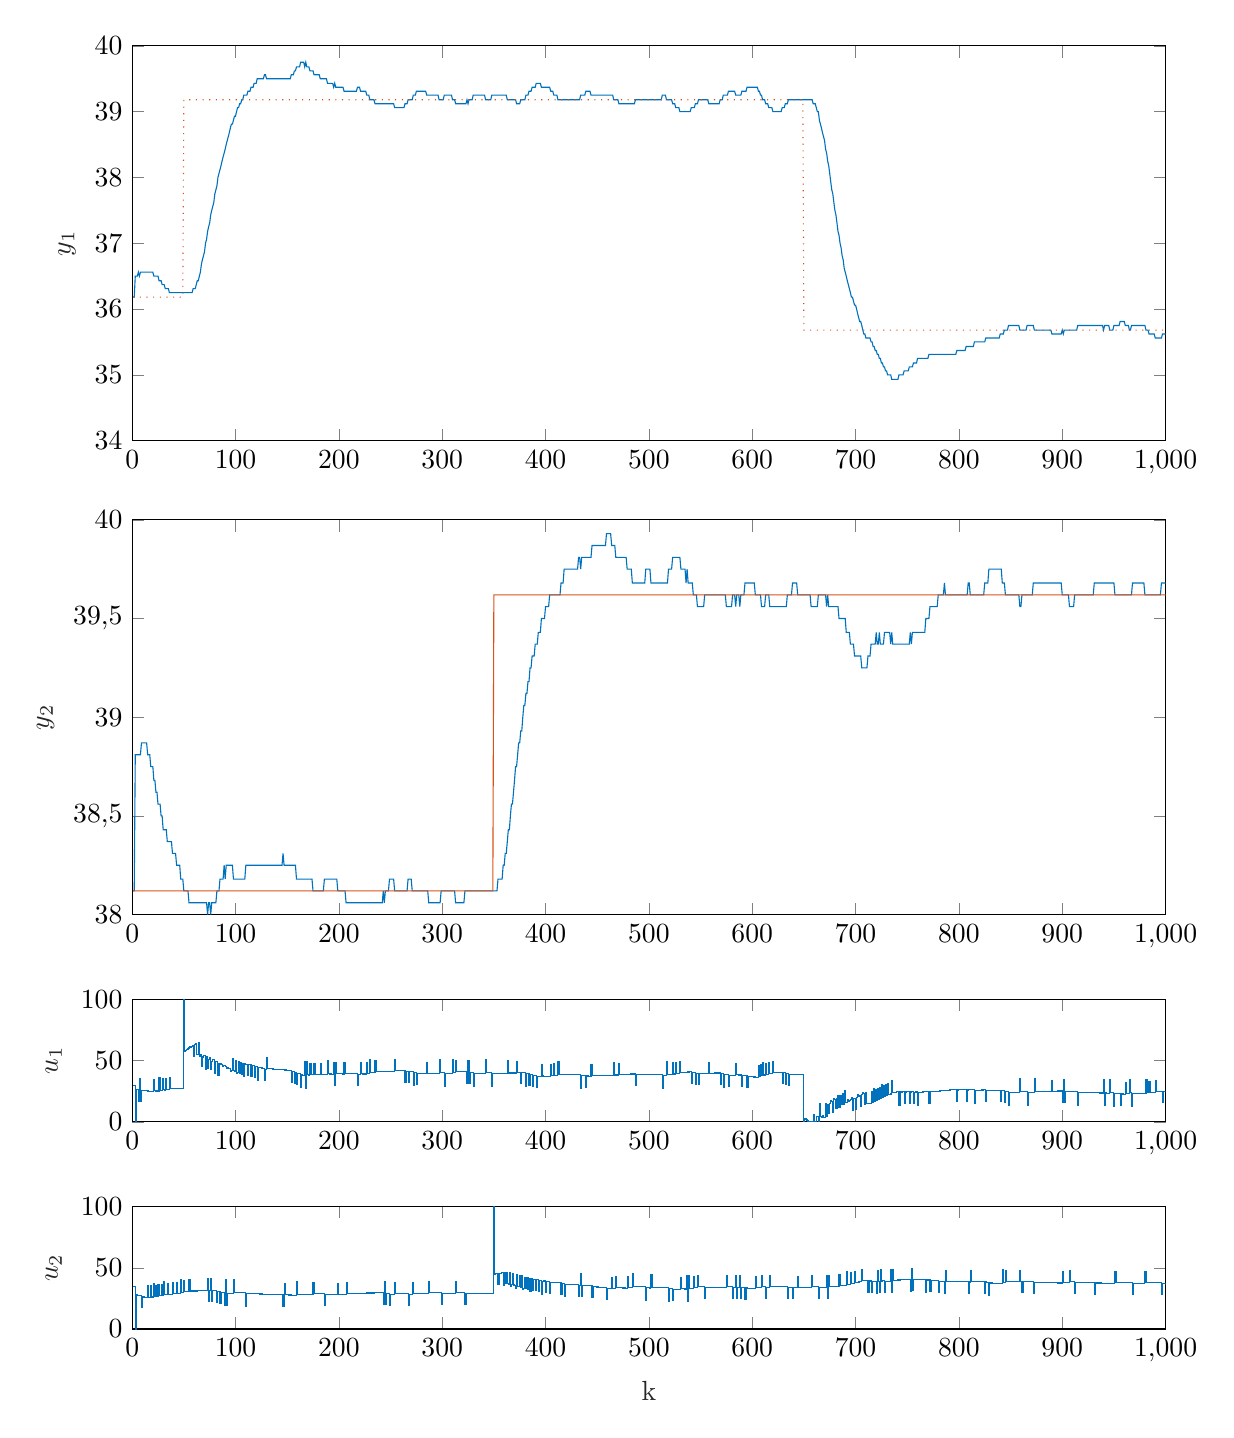
\begin{tikzpicture}

\begin{axis}[%
width=5.167in,
height=0.612in,
at={(0.646in,0.494in)},
scale only axis,
xmin=0,
xmax=1000,
xtick={0,100,200,300,400,500,600,700,800,900,1000},
xlabel style={font=\color{white!15!black}},
xlabel={k},
ymin=0,
ymax=100,
ytick={0,50,100},
ylabel style={font=\color{white!15!black}},
ylabel={$\text{u}_\text{2}$},
axis background/.style={fill=white}
]
\addplot[const plot, color=mycolor1, forget plot] table[row sep=crcr] {%
1	35\\
2	35\\
3	0\\
4	27.87\\
5	27.7167\\
6	27.5633\\
7	27.41\\
8	27.2567\\
9	17.497\\
10	26.33\\
11	26.1633\\
12	25.9967\\
13	25.83\\
14	25.6633\\
15	35.10333\\
16	25.95\\
17	25.7967\\
18	35.25\\
19	26.11\\
20	25.97\\
21	37.0378\\
22	26.4133\\
23	35.89556\\
24	26.7844\\
25	36.28\\
26	27.1822\\
27	27.0844\\
28	36.5933\\
29	27.5089\\
30	38.6322\\
31	28.0633\\
32	27.9944\\
33	27.9256\\
34	37.4633\\
35	28.4078\\
36	28.3522\\
37	28.2967\\
38	28.2411\\
39	37.7922\\
40	28.75\\
41	28.7078\\
42	28.6656\\
43	38.23\\
44	29.2011\\
45	29.1722\\
46	29.1433\\
47	40.3222\\
48	29.8089\\
49	29.7956\\
50	39.3889\\
51	30.3889\\
52	30.3889\\
53	30.3889\\
54	30.3889\\
55	39.9956\\
56	31.0089\\
57	31.0222\\
58	31.0356\\
59	31.0489\\
60	31.0622\\
61	31.0756\\
62	31.0889\\
63	31.1022\\
64	31.1156\\
65	31.1289\\
66	31.1422\\
67	31.1556\\
68	31.1689\\
69	31.1822\\
70	31.1956\\
71	31.2089\\
72	31.2222\\
73	40.8422\\
74	22.262\\
75	31.2756\\
76	40.8956\\
77	22.316\\
78	31.3289\\
79	31.3422\\
80	31.3556\\
81	31.3689\\
82	21.776\\
83	30.7756\\
84	30.7756\\
85	21.169\\
86	30.1556\\
87	30.1422\\
88	30.1289\\
89	18.908\\
90	40.5867\\
91	18.866\\
92	29.3367\\
93	29.3078\\
94	29.2789\\
95	29.25\\
96	29.2211\\
97	29.1922\\
98	40.3711\\
99	29.8578\\
100	29.8444\\
101	29.8311\\
102	29.8178\\
103	29.8044\\
104	29.7911\\
105	29.7778\\
106	29.7644\\
107	29.7511\\
108	29.7378\\
109	29.7244\\
110	18.503\\
111	28.9744\\
112	28.9456\\
113	28.9167\\
114	28.8878\\
115	28.8589\\
116	28.83\\
117	28.8011\\
118	28.7722\\
119	28.7433\\
120	28.7144\\
121	28.6856\\
122	28.6567\\
123	28.6278\\
124	28.5989\\
125	28.57\\
126	28.5411\\
127	28.5122\\
128	28.4833\\
129	28.4544\\
130	28.4256\\
131	28.3967\\
132	28.3678\\
133	28.3389\\
134	28.31\\
135	28.2811\\
136	28.2522\\
137	28.2233\\
138	28.1944\\
139	28.1656\\
140	28.1367\\
141	28.1078\\
142	28.0789\\
143	28.05\\
144	28.0211\\
145	27.9922\\
146	18.357\\
147	36.9211\\
148	27.8922\\
149	27.8633\\
150	27.8344\\
151	27.8056\\
152	27.7767\\
153	27.7478\\
154	27.7189\\
155	27.69\\
156	27.6611\\
157	27.6322\\
158	27.6033\\
159	38.7822\\
160	28.2689\\
161	28.2556\\
162	28.2422\\
163	28.2289\\
164	28.2156\\
165	28.2022\\
166	28.1889\\
167	28.1756\\
168	28.1622\\
169	28.1489\\
170	28.1356\\
171	28.1222\\
172	28.1089\\
173	28.0956\\
174	28.0822\\
175	37.6756\\
176	28.6756\\
177	28.6756\\
178	28.6756\\
179	28.6756\\
180	28.6756\\
181	28.6756\\
182	28.6756\\
183	28.6756\\
184	28.6756\\
185	28.6756\\
186	19.069\\
187	28.0556\\
188	28.0422\\
189	28.0289\\
190	28.0156\\
191	28.0022\\
192	27.9889\\
193	27.9756\\
194	27.9622\\
195	27.9489\\
196	27.9356\\
197	27.9222\\
198	27.9089\\
199	37.5022\\
200	28.5022\\
201	28.5022\\
202	28.5022\\
203	28.5022\\
204	28.5022\\
205	28.5022\\
206	28.5022\\
207	38.1089\\
208	29.1222\\
209	29.1356\\
210	29.1489\\
211	29.1622\\
212	29.1756\\
213	29.1889\\
214	29.2022\\
215	29.2156\\
216	29.2289\\
217	29.2422\\
218	29.2556\\
219	29.2689\\
220	29.2822\\
221	29.2956\\
222	29.3089\\
223	29.3222\\
224	29.3356\\
225	29.3489\\
226	29.3622\\
227	29.3756\\
228	29.3889\\
229	29.4022\\
230	29.4156\\
231	29.4289\\
232	29.4422\\
233	29.4556\\
234	29.4689\\
235	29.4822\\
236	29.4956\\
237	29.5089\\
238	29.5222\\
239	29.5356\\
240	29.5489\\
241	29.5622\\
242	29.5756\\
243	19.982\\
244	38.5889\\
245	19.996\\
246	28.9956\\
247	28.9956\\
248	28.9956\\
249	19.389\\
250	28.3756\\
251	28.3622\\
252	28.3489\\
253	28.3356\\
254	37.9289\\
255	28.9289\\
256	28.9289\\
257	28.9289\\
258	28.9289\\
259	28.9289\\
260	28.9289\\
261	28.9289\\
262	28.9289\\
263	28.9289\\
264	28.9289\\
265	28.9289\\
266	28.9289\\
267	19.322\\
268	28.3089\\
269	28.2956\\
270	28.2822\\
271	37.8756\\
272	28.8756\\
273	28.8756\\
274	28.8756\\
275	28.8756\\
276	28.8756\\
277	28.8756\\
278	28.8756\\
279	28.8756\\
280	28.8756\\
281	28.8756\\
282	28.8756\\
283	28.8756\\
284	28.8756\\
285	28.8756\\
286	28.8756\\
287	38.4822\\
288	29.4956\\
289	29.5089\\
290	29.5222\\
291	29.5356\\
292	29.5489\\
293	29.5622\\
294	29.5756\\
295	29.5889\\
296	29.6022\\
297	29.6156\\
298	29.6289\\
299	20.036\\
300	29.0356\\
301	29.0356\\
302	29.0356\\
303	29.0356\\
304	29.0356\\
305	29.0356\\
306	29.0356\\
307	29.0356\\
308	29.0356\\
309	29.0356\\
310	29.0356\\
311	29.0356\\
312	29.0356\\
313	38.6422\\
314	29.6556\\
315	29.6689\\
316	29.6822\\
317	29.6956\\
318	29.7089\\
319	29.7222\\
320	29.7356\\
321	29.7489\\
322	20.156\\
323	29.1556\\
324	29.1556\\
325	29.1556\\
326	29.1556\\
327	29.1556\\
328	29.1556\\
329	29.1556\\
330	29.1556\\
331	29.1556\\
332	29.1556\\
333	29.1556\\
334	29.1556\\
335	29.1556\\
336	29.1556\\
337	29.1556\\
338	29.1556\\
339	29.1556\\
340	29.1556\\
341	29.1556\\
342	29.1556\\
343	29.1556\\
344	29.1556\\
345	29.1556\\
346	29.1556\\
347	29.1556\\
348	29.1556\\
349	29.1556\\
350	100\\
351	44.6556\\
352	44.9889\\
353	45.322\\
354	36.0489\\
355	45.369\\
356	45.689\\
357	46.009\\
358	46.329\\
359	35.44111\\
360	46.246\\
361	36.9433\\
362	46.234\\
363	36.9189\\
364	36.59\\
365	45.854\\
366	34.911111\\
367	36.0533\\
368	45.289\\
369	35.91778\\
370	35.53333\\
371	33.5344\\
372	44.2278\\
373	34.81444\\
374	34.38778\\
375	43.5544\\
376	34.11444\\
377	43.2678\\
378	32.2133\\
379	33.2444\\
380	42.3689\\
381	32.8867\\
382	41.9978\\
383	32.5022\\
384	41.6\\
385	30.49\\
386	41.0722\\
387	31.5478\\
388	40.6167\\
389	40.6856\\
390	31.1478\\
391	40.2033\\
392	40.2589\\
393	30.7078\\
394	39.75\\
395	39.7922\\
396	28.6267\\
397	39.1533\\
398	39.18\\
399	39.2067\\
400	29.6267\\
401	38.64\\
402	38.6533\\
403	38.6667\\
404	29.0733\\
405	38.0733\\
406	38.0733\\
407	38.0733\\
408	38.0733\\
409	38.0733\\
410	38.0733\\
411	38.0733\\
412	38.0733\\
413	38.0733\\
414	38.0733\\
415	28.4667\\
416	37.4533\\
417	37.44\\
418	26.2189\\
419	36.69\\
420	36.6611\\
421	36.6322\\
422	36.6033\\
423	36.5744\\
424	36.5456\\
425	36.5167\\
426	36.4878\\
427	36.4589\\
428	36.43\\
429	36.4011\\
430	36.3722\\
431	36.3433\\
432	26.7078\\
433	35.66556\\
434	45.23\\
435	26.5944\\
436	35.55222\\
437	35.51\\
438	35.46778\\
439	35.42556\\
440	35.38333\\
441	35.34111\\
442	35.29889\\
443	35.25667\\
444	35.21444\\
445	25.5656\\
446	34.51\\
447	34.45444\\
448	34.39889\\
449	34.34333\\
450	34.28778\\
451	34.23222\\
452	34.17667\\
453	34.12111\\
454	34.06556\\
455	34.01\\
456	33.9544\\
457	33.8989\\
458	33.8433\\
459	24.181\\
460	33.1122\\
461	33.0433\\
462	32.9744\\
463	32.9056\\
464	42.4433\\
465	33.3878\\
466	33.3322\\
467	33.2767\\
468	42.8278\\
469	33.7856\\
470	33.7433\\
471	33.7011\\
472	33.6589\\
473	33.6167\\
474	33.5744\\
475	33.5322\\
476	33.49\\
477	33.4478\\
478	33.4056\\
479	42.97\\
480	33.9411\\
481	33.9122\\
482	33.8833\\
483	33.8544\\
484	45.033\\
485	34.52\\
486	34.50667\\
487	34.49333\\
488	34.48\\
489	34.46667\\
490	34.45333\\
491	34.44\\
492	34.42667\\
493	34.41333\\
494	34.4\\
495	34.38667\\
496	34.37333\\
497	23.152\\
498	33.6233\\
499	33.5944\\
500	33.5656\\
501	33.5367\\
502	44.7156\\
503	34.20222\\
504	34.18889\\
505	34.17556\\
506	34.16222\\
507	34.14889\\
508	34.13556\\
509	34.12222\\
510	34.10889\\
511	34.09556\\
512	34.08222\\
513	34.06889\\
514	34.05556\\
515	34.04222\\
516	34.02889\\
517	34.01556\\
518	34.00222\\
519	22.781\\
520	33.2522\\
521	33.2233\\
522	33.1944\\
523	23.559\\
524	32.5167\\
525	32.4744\\
526	32.4322\\
527	32.39\\
528	32.3478\\
529	32.3056\\
530	32.2633\\
531	41.8278\\
532	32.7989\\
533	32.77\\
534	32.7411\\
535	32.7122\\
536	43.8911\\
537	22.17\\
538	43.8489\\
539	33.3356\\
540	33.3222\\
541	33.3089\\
542	33.2956\\
543	42.8889\\
544	33.8889\\
545	33.8889\\
546	33.8889\\
547	43.4956\\
548	34.50889\\
549	34.52222\\
550	34.53556\\
551	34.54889\\
552	34.56222\\
553	34.57556\\
554	24.982\\
555	33.9822\\
556	33.9822\\
557	33.9822\\
558	33.9822\\
559	33.9822\\
560	33.9822\\
561	33.9822\\
562	33.9822\\
563	33.9822\\
564	33.9822\\
565	33.9822\\
566	33.9822\\
567	33.9822\\
568	33.9822\\
569	33.9822\\
570	33.9822\\
571	33.9822\\
572	33.9822\\
573	33.9822\\
574	33.9822\\
575	43.5889\\
576	34.60222\\
577	34.61556\\
578	34.62889\\
579	34.64222\\
580	34.65556\\
581	25.0622\\
582	34.06222\\
583	34.06222\\
584	43.6689\\
585	25.0756\\
586	34.07556\\
587	34.07556\\
588	43.6822\\
589	25.0889\\
590	34.08889\\
591	34.08889\\
592	34.08889\\
593	24.482\\
594	33.4689\\
595	33.4556\\
596	33.4422\\
597	33.4289\\
598	33.4156\\
599	33.4022\\
600	33.3889\\
601	33.3756\\
602	33.3622\\
603	42.9556\\
604	33.9556\\
605	33.9556\\
606	33.9556\\
607	33.9556\\
608	33.9556\\
609	43.5622\\
610	34.57556\\
611	34.58889\\
612	34.60222\\
613	25.0089\\
614	34.00889\\
615	34.00889\\
616	34.00889\\
617	43.6156\\
618	34.62889\\
619	34.64222\\
620	34.65556\\
621	34.66889\\
622	34.68222\\
623	34.69556\\
624	34.70889\\
625	34.72222\\
626	34.73556\\
627	34.74889\\
628	34.76222\\
629	34.77556\\
630	34.78889\\
631	34.80222\\
632	34.81556\\
633	34.82889\\
634	25.2356\\
635	34.23556\\
636	34.23556\\
637	34.23556\\
638	34.23556\\
639	24.629\\
640	33.6156\\
641	33.6022\\
642	33.5889\\
643	33.5756\\
644	43.1689\\
645	34.16889\\
646	34.16889\\
647	34.16889\\
648	34.16889\\
649	34.16889\\
650	34.16889\\
651	34.16889\\
652	34.16889\\
653	34.16889\\
654	34.16889\\
655	34.16889\\
656	34.16889\\
657	43.7756\\
658	34.78889\\
659	34.80222\\
660	34.81556\\
661	34.82889\\
662	34.84222\\
663	34.85556\\
664	25.2622\\
665	34.26222\\
666	34.26222\\
667	34.26222\\
668	34.26222\\
669	34.26222\\
670	34.26222\\
671	34.26222\\
672	43.8689\\
673	25.2756\\
674	43.8822\\
675	34.89556\\
676	34.908889\\
677	34.922222\\
678	34.935556\\
679	34.948889\\
680	34.962222\\
681	34.975556\\
682	34.988889\\
683	35.0022222\\
684	44.6222\\
685	35.64889\\
686	35.67556\\
687	35.70222\\
688	35.72889\\
689	35.75556\\
690	35.78222\\
691	47.017\\
692	36.5589\\
693	36.6011\\
694	36.6433\\
695	46.292\\
696	37.3478\\
697	37.4033\\
698	37.4589\\
699	47.121\\
700	38.19\\
701	38.2589\\
702	38.3278\\
703	38.3967\\
704	38.4656\\
705	38.5344\\
706	48.21\\
707	39.2922\\
708	39.3744\\
709	39.4567\\
710	39.5389\\
711	39.6211\\
712	30.0967\\
713	39.1656\\
714	39.2344\\
715	29.6967\\
716	38.7522\\
717	38.8078\\
718	38.8633\\
719	38.9189\\
720	29.3678\\
721	48.017\\
722	39.0722\\
723	29.5211\\
724	48.17\\
725	39.2256\\
726	39.2811\\
727	39.3367\\
728	29.7856\\
729	38.8278\\
730	38.87\\
731	38.9122\\
732	38.9544\\
733	38.9967\\
734	48.646\\
735	30.0944\\
736	48.743\\
737	39.7989\\
738	39.8544\\
739	39.91\\
740	39.9656\\
741	40.0211\\
742	40.0767\\
743	40.1322\\
744	40.1878\\
745	40.2433\\
746	40.2989\\
747	40.3544\\
748	40.41\\
749	40.4656\\
750	40.5211\\
751	40.5767\\
752	40.6322\\
753	31.0811\\
754	49.73\\
755	31.1789\\
756	40.2211\\
757	40.2633\\
758	40.3056\\
759	40.3478\\
760	40.39\\
761	40.4322\\
762	40.4744\\
763	40.5167\\
764	40.5589\\
765	40.6011\\
766	40.6433\\
767	40.6856\\
768	29.52\\
769	40.0467\\
770	40.0733\\
771	40.1\\
772	30.52\\
773	39.5333\\
774	39.5467\\
775	39.56\\
776	39.5733\\
777	39.5867\\
778	39.6\\
779	39.6133\\
780	30.02\\
781	39.02\\
782	39.02\\
783	39.02\\
784	39.02\\
785	39.02\\
786	29.4133\\
787	48.007\\
788	39.0067\\
789	39.0067\\
790	39.0067\\
791	39.0067\\
792	39.0067\\
793	39.0067\\
794	39.0067\\
795	39.0067\\
796	39.0067\\
797	39.0067\\
798	39.0067\\
799	39.0067\\
800	39.0067\\
801	39.0067\\
802	39.0067\\
803	39.0067\\
804	39.0067\\
805	39.0067\\
806	39.0067\\
807	39.0067\\
808	39.0067\\
809	29.4\\
810	38.3867\\
811	47.98\\
812	38.98\\
813	38.98\\
814	38.98\\
815	38.98\\
816	38.98\\
817	38.98\\
818	38.98\\
819	38.98\\
820	38.98\\
821	38.98\\
822	38.98\\
823	38.98\\
824	38.98\\
825	29.3733\\
826	38.36\\
827	38.3467\\
828	38.3333\\
829	27.1122\\
830	37.5833\\
831	37.5544\\
832	37.5256\\
833	37.4967\\
834	37.4678\\
835	37.4389\\
836	37.41\\
837	37.3811\\
838	37.3522\\
839	37.3233\\
840	37.2944\\
841	37.2656\\
842	48.444\\
843	37.9311\\
844	37.9178\\
845	47.511\\
846	38.5111\\
847	38.5111\\
848	38.5111\\
849	38.5111\\
850	38.5111\\
851	38.5111\\
852	38.5111\\
853	38.5111\\
854	38.5111\\
855	38.5111\\
856	38.5111\\
857	38.5111\\
858	38.5111\\
859	48.118\\
860	39.1311\\
861	29.5378\\
862	38.5378\\
863	38.5378\\
864	38.5378\\
865	38.5378\\
866	38.5378\\
867	38.5378\\
868	38.5378\\
869	38.5378\\
870	38.5378\\
871	38.5378\\
872	28.9311\\
873	37.9178\\
874	37.9044\\
875	37.8911\\
876	37.8778\\
877	37.8644\\
878	37.8511\\
879	37.8378\\
880	37.8244\\
881	37.8111\\
882	37.7978\\
883	37.7844\\
884	37.7711\\
885	37.7578\\
886	37.7444\\
887	37.7311\\
888	37.7178\\
889	37.7044\\
890	37.6911\\
891	37.6778\\
892	37.6644\\
893	37.6511\\
894	37.6378\\
895	37.6244\\
896	37.6111\\
897	37.5978\\
898	37.5844\\
899	37.5711\\
900	47.164\\
901	38.1644\\
902	38.1644\\
903	38.1644\\
904	38.1644\\
905	38.1644\\
906	38.1644\\
907	47.771\\
908	38.7844\\
909	38.7978\\
910	38.8111\\
911	38.8244\\
912	29.2311\\
913	38.2311\\
914	38.2311\\
915	38.2311\\
916	38.2311\\
917	38.2311\\
918	38.2311\\
919	38.2311\\
920	38.2311\\
921	38.2311\\
922	38.2311\\
923	38.2311\\
924	38.2311\\
925	38.2311\\
926	38.2311\\
927	38.2311\\
928	38.2311\\
929	38.2311\\
930	38.2311\\
931	28.6244\\
932	37.6111\\
933	37.5978\\
934	37.5844\\
935	37.5711\\
936	37.5578\\
937	37.5444\\
938	37.5311\\
939	37.5178\\
940	37.5044\\
941	37.4911\\
942	37.4778\\
943	37.4644\\
944	37.4511\\
945	37.4378\\
946	37.4244\\
947	37.4111\\
948	37.3978\\
949	37.3844\\
950	37.3711\\
951	46.964\\
952	37.9644\\
953	37.9644\\
954	37.9644\\
955	37.9644\\
956	37.9644\\
957	37.9644\\
958	37.9644\\
959	37.9644\\
960	37.9644\\
961	37.9644\\
962	37.9644\\
963	37.9644\\
964	37.9644\\
965	37.9644\\
966	37.9644\\
967	37.9644\\
968	28.3578\\
969	37.3444\\
970	37.3311\\
971	37.3178\\
972	37.3044\\
973	37.2911\\
974	37.2778\\
975	37.2644\\
976	37.2511\\
977	37.2378\\
978	37.2244\\
979	37.2111\\
980	46.804\\
981	37.8044\\
982	37.8044\\
983	37.8044\\
984	37.8044\\
985	37.8044\\
986	37.8044\\
987	37.8044\\
988	37.8044\\
989	37.8044\\
990	37.8044\\
991	37.8044\\
992	37.8044\\
993	37.8044\\
994	37.8044\\
995	37.8044\\
996	28.1978\\
997	37.1844\\
998	37.1711\\
999	37.1578\\
1000	37.1444\\
};
\end{axis}

\begin{axis}[%
width=5.167in,
height=0.612in,
at={(0.646in,1.53in)},
scale only axis,
xmin=0,
xmax=1000,
xtick={0,100,200,300,400,500,600,700,800,900,1000},
ymin=0,
ymax=100,
ytick={0,50,100},
ylabel style={font=\color{white!15!black}},
ylabel={$\text{u}_\text{1}$},
axis background/.style={fill=white}
]
\addplot[const plot, color=mycolor1, forget plot] table[row sep=crcr] {%
1	30\\
2	30\\
3	0\\
4	26.6933\\
5	26.6222\\
6	16.944\\
7	35.4667\\
8	16.789\\
9	25.7044\\
10	25.62\\
11	25.5356\\
12	25.4511\\
13	25.3667\\
14	25.2822\\
15	25.1978\\
16	25.1133\\
17	25.0289\\
18	24.9444\\
19	24.86\\
20	24.7756\\
21	34.2978\\
22	25.2267\\
23	25.1556\\
24	25.0844\\
25	25.0133\\
26	36.15\\
27	25.5944\\
28	25.5389\\
29	35.09\\
30	26.0478\\
31	26.0056\\
32	35.57\\
33	26.5411\\
34	26.5122\\
35	26.4833\\
36	36.0611\\
37	27.0456\\
38	27.03\\
39	27.0144\\
40	26.9989\\
41	26.9833\\
42	26.9678\\
43	26.9522\\
44	26.9367\\
45	26.9211\\
46	26.9056\\
47	26.89\\
48	26.8744\\
49	26.8589\\
50	100\\
51	57.828\\
52	58.479\\
53	59.13\\
54	59.781\\
55	60.432\\
56	61.083\\
57	61.734\\
58	62.386\\
59	53.43\\
60	63.068\\
61	63.706\\
62	54.737\\
63	54.754\\
64	64.366\\
65	53.769\\
66	55.258\\
67	45.627\\
68	52.974\\
69	54.408\\
70	54.328\\
71	43.027\\
72	53.404\\
73	43.662\\
74	50.899\\
75	52.221\\
76	42.423\\
77	49.604\\
78	50.871\\
79	50.624\\
80	39.1567\\
81	49.368\\
82	49.066\\
83	37.5422\\
84	47.698\\
85	47.34\\
86	46.969\\
87	44.983\\
88	46.083\\
89	45.67\\
90	45.243\\
91	43.202\\
92	44.247\\
93	43.778\\
94	43.296\\
95	41.199\\
96	42.188\\
97	51.27\\
98	41.746\\
99	41.208\\
100	50.263\\
101	39.1111\\
102	40.044\\
103	49.071\\
104	39.4911\\
105	48.504\\
106	38.9111\\
107	47.911\\
108	36.7033\\
109	47.188\\
110	47.172\\
111	47.157\\
112	37.5344\\
113	46.506\\
114	46.477\\
115	36.8411\\
116	45.799\\
117	45.757\\
118	36.1078\\
119	45.052\\
120	44.997\\
121	33.7333\\
122	44.162\\
123	44.091\\
124	44.02\\
125	43.949\\
126	43.878\\
127	43.807\\
128	34.1289\\
129	43.044\\
130	52.567\\
131	43.496\\
132	43.424\\
133	43.353\\
134	43.282\\
135	43.211\\
136	43.14\\
137	43.069\\
138	42.998\\
139	42.927\\
140	42.856\\
141	42.784\\
142	42.713\\
143	42.642\\
144	42.571\\
145	42.5\\
146	42.429\\
147	42.358\\
148	42.287\\
149	42.216\\
150	42.144\\
151	42.073\\
152	42.002\\
153	41.931\\
154	32.2533\\
155	41.169\\
156	41.084\\
157	31.3933\\
158	40.296\\
159	30.59111\\
160	39.48\\
161	39.3689\\
162	39.2578\\
163	27.9389\\
164	38.3122\\
165	38.1856\\
166	38.0589\\
167	49.14\\
168	27.3211\\
169	48.902\\
170	38.2911\\
171	38.18\\
172	47.676\\
173	38.5778\\
174	38.48\\
175	38.3822\\
176	47.891\\
177	38.8067\\
178	38.7222\\
179	38.6378\\
180	38.5533\\
181	38.4689\\
182	47.991\\
183	38.92\\
184	38.8489\\
185	38.7778\\
186	38.7067\\
187	38.6356\\
188	38.5644\\
189	49.701\\
190	39.1456\\
191	39.09\\
192	39.0344\\
193	38.9789\\
194	38.9233\\
195	48.474\\
196	29.82556\\
197	48.377\\
198	39.3344\\
199	39.2922\\
200	39.25\\
201	39.2078\\
202	39.1656\\
203	39.1233\\
204	39.0811\\
205	48.646\\
206	39.6167\\
207	39.5878\\
208	39.5589\\
209	39.53\\
210	39.5011\\
211	39.4722\\
212	39.4433\\
213	39.4144\\
214	39.3856\\
215	39.3567\\
216	39.3278\\
217	39.2989\\
218	29.66333\\
219	38.6211\\
220	38.5789\\
221	48.143\\
222	39.1144\\
223	39.0856\\
224	39.0567\\
225	39.0278\\
226	38.9989\\
227	48.577\\
228	39.5611\\
229	39.5456\\
230	50.738\\
231	40.238\\
232	40.238\\
233	40.238\\
234	40.238\\
235	49.844\\
236	40.858\\
237	40.871\\
238	40.884\\
239	40.898\\
240	40.911\\
241	40.924\\
242	40.938\\
243	40.951\\
244	40.964\\
245	40.978\\
246	40.991\\
247	41.004\\
248	41.018\\
249	41.031\\
250	41.044\\
251	41.058\\
252	41.071\\
253	41.084\\
254	50.704\\
255	41.731\\
256	41.758\\
257	41.784\\
258	41.811\\
259	41.838\\
260	41.864\\
261	41.891\\
262	41.918\\
263	41.944\\
264	32.3644\\
265	41.378\\
266	41.391\\
267	31.7978\\
268	40.798\\
269	40.798\\
270	40.798\\
271	40.798\\
272	29.59\\
273	40.074\\
274	40.059\\
275	30.43667\\
276	39.4078\\
277	39.3789\\
278	39.35\\
279	39.3211\\
280	39.2922\\
281	39.2633\\
282	39.2344\\
283	39.2056\\
284	39.1767\\
285	48.754\\
286	39.7389\\
287	39.7233\\
288	39.7078\\
289	39.6922\\
290	39.6767\\
291	39.6611\\
292	39.6456\\
293	39.63\\
294	39.6144\\
295	39.5989\\
296	39.5833\\
297	50.776\\
298	40.276\\
299	40.276\\
300	40.276\\
301	40.276\\
302	29.06778\\
303	39.5522\\
304	39.5367\\
305	39.5211\\
306	39.5056\\
307	39.49\\
308	39.4744\\
309	39.4589\\
310	50.651\\
311	40.151\\
312	40.151\\
313	49.758\\
314	40.771\\
315	40.784\\
316	40.798\\
317	40.811\\
318	40.824\\
319	40.838\\
320	40.851\\
321	40.864\\
322	40.878\\
323	40.891\\
324	31.2978\\
325	49.904\\
326	31.3111\\
327	40.311\\
328	40.311\\
329	40.311\\
330	29.10333\\
331	39.5878\\
332	39.5722\\
333	39.5567\\
334	39.5411\\
335	39.5256\\
336	39.51\\
337	39.4944\\
338	39.4789\\
339	39.4633\\
340	39.4478\\
341	39.4322\\
342	50.624\\
343	40.124\\
344	40.124\\
345	40.124\\
346	40.124\\
347	40.124\\
348	28.9167\\
349	39.4011\\
350	39.3856\\
351	39.37\\
352	39.3544\\
353	39.3389\\
354	39.3233\\
355	39.3078\\
356	39.2922\\
357	39.2767\\
358	39.2611\\
359	39.2456\\
360	39.23\\
361	39.2144\\
362	39.1989\\
363	50.391\\
364	39.8911\\
365	39.8911\\
366	39.8911\\
367	39.8911\\
368	39.8911\\
369	39.8911\\
370	39.8911\\
371	39.8911\\
372	49.498\\
373	40.511\\
374	40.524\\
375	40.538\\
376	30.94444\\
377	39.9444\\
378	39.9444\\
379	39.9444\\
380	39.9444\\
381	28.7367\\
382	39.2211\\
383	39.2056\\
384	29.58333\\
385	38.5544\\
386	38.5256\\
387	28.89\\
388	37.8478\\
389	37.8056\\
390	37.7633\\
391	28.1144\\
392	37.0589\\
393	37.0033\\
394	36.9478\\
395	36.8922\\
396	46.443\\
397	37.4011\\
398	37.3589\\
399	37.3167\\
400	37.2744\\
401	37.2322\\
402	37.19\\
403	37.1478\\
404	37.1056\\
405	46.67\\
406	37.6411\\
407	37.6122\\
408	47.19\\
409	38.1744\\
410	38.1589\\
411	38.1433\\
412	49.336\\
413	38.8356\\
414	38.8356\\
415	38.8356\\
416	38.8356\\
417	38.8356\\
418	38.8356\\
419	38.8356\\
420	38.8356\\
421	38.8356\\
422	38.8356\\
423	38.8356\\
424	38.8356\\
425	38.8356\\
426	38.8356\\
427	38.8356\\
428	38.8356\\
429	38.8356\\
430	38.8356\\
431	38.8356\\
432	38.8356\\
433	38.8356\\
434	27.6278\\
435	38.1122\\
436	38.0967\\
437	38.0811\\
438	38.0656\\
439	28.4433\\
440	37.4144\\
441	37.3856\\
442	37.3567\\
443	37.3278\\
444	46.906\\
445	37.89\\
446	37.8744\\
447	37.8589\\
448	37.8433\\
449	37.8278\\
450	37.8122\\
451	37.7967\\
452	37.7811\\
453	37.7656\\
454	37.75\\
455	37.7344\\
456	37.7189\\
457	37.7033\\
458	37.6878\\
459	37.6722\\
460	37.6567\\
461	37.6411\\
462	37.6256\\
463	37.61\\
464	37.5944\\
465	37.5789\\
466	48.771\\
467	38.2711\\
468	38.2711\\
469	38.2711\\
470	38.2711\\
471	47.878\\
472	38.8911\\
473	38.9044\\
474	38.9178\\
475	38.9311\\
476	38.9444\\
477	38.9578\\
478	38.9711\\
479	38.9844\\
480	38.9978\\
481	39.0111\\
482	39.0244\\
483	39.0378\\
484	39.0511\\
485	39.0644\\
486	39.0778\\
487	29.48444\\
488	38.4844\\
489	38.4844\\
490	38.4844\\
491	38.4844\\
492	38.4844\\
493	38.4844\\
494	38.4844\\
495	38.4844\\
496	38.4844\\
497	38.4844\\
498	38.4844\\
499	38.4844\\
500	38.4844\\
501	38.4844\\
502	38.4844\\
503	38.4844\\
504	38.4844\\
505	38.4844\\
506	38.4844\\
507	38.4844\\
508	38.4844\\
509	38.4844\\
510	38.4844\\
511	38.4844\\
512	38.4844\\
513	27.2767\\
514	37.7611\\
515	37.7456\\
516	37.73\\
517	48.922\\
518	38.4222\\
519	38.4222\\
520	38.4222\\
521	38.4222\\
522	38.4222\\
523	48.029\\
524	39.0422\\
525	39.0556\\
526	48.676\\
527	39.7022\\
528	39.7289\\
529	39.7556\\
530	49.389\\
531	40.429\\
532	40.469\\
533	40.509\\
534	40.549\\
535	40.589\\
536	40.629\\
537	40.669\\
538	40.709\\
539	40.749\\
540	40.789\\
541	31.2222\\
542	40.249\\
543	40.276\\
544	40.302\\
545	30.72222\\
546	39.7356\\
547	39.7489\\
548	30.15556\\
549	39.1556\\
550	39.1556\\
551	39.1556\\
552	39.1556\\
553	39.1556\\
554	39.1556\\
555	39.1556\\
556	39.1556\\
557	39.1556\\
558	48.762\\
559	39.7756\\
560	39.7889\\
561	39.8022\\
562	39.8156\\
563	39.8289\\
564	39.8422\\
565	39.8556\\
566	39.8689\\
567	39.8822\\
568	39.8956\\
569	30.30222\\
570	39.3022\\
571	39.3022\\
572	28.0944\\
573	38.5789\\
574	38.5633\\
575	38.5478\\
576	38.5322\\
577	28.91\\
578	37.8811\\
579	37.8522\\
580	37.8233\\
581	37.7944\\
582	37.7656\\
583	37.7367\\
584	47.314\\
585	38.2989\\
586	38.2833\\
587	38.2678\\
588	38.2522\\
589	38.2367\\
590	28.6144\\
591	37.5856\\
592	37.5567\\
593	37.5278\\
594	37.4989\\
595	27.8633\\
596	36.8211\\
597	36.7789\\
598	36.7367\\
599	36.6944\\
600	36.6522\\
601	36.61\\
602	36.5678\\
603	36.5256\\
604	36.4833\\
605	36.4411\\
606	46.006\\
607	36.9767\\
608	46.554\\
609	37.5389\\
610	48.731\\
611	38.2311\\
612	38.2311\\
613	47.838\\
614	38.8511\\
615	38.8644\\
616	48.484\\
617	39.5111\\
618	39.5378\\
619	39.5644\\
620	49.198\\
621	40.238\\
622	40.278\\
623	40.318\\
624	40.358\\
625	40.398\\
626	40.438\\
627	40.478\\
628	40.518\\
629	30.95111\\
630	39.9778\\
631	40.004\\
632	30.42444\\
633	39.4378\\
634	39.4511\\
635	29.85778\\
636	38.8578\\
637	38.8578\\
638	38.8578\\
639	38.8578\\
640	38.8578\\
641	38.8578\\
642	38.8578\\
643	38.8578\\
644	38.8578\\
645	38.8578\\
646	38.8578\\
647	38.8578\\
648	38.8578\\
649	38.8578\\
650	0\\
651	2.691\\
652	1.913\\
653	1.136\\
654	0.358000000000001\\
655	0\\
656	0\\
657	0\\
658	0\\
659	6.076\\
660	0\\
661	0\\
662	4.389\\
663	4.244\\
664	0\\
665	14.583\\
666	3.981\\
667	3.892\\
668	5.418\\
669	3.858\\
670	3.811\\
671	14.986\\
672	4.481\\
673	14.097\\
674	6.733\\
675	14.891\\
676	17.177\\
677	16.39\\
678	7.523\\
679	18.878\\
680	18.16\\
681	10.963\\
682	19.288\\
683	21.74\\
684	11.513\\
685	21.4067\\
686	14.321\\
687	22.7567\\
688	14.112\\
689	25.6889\\
690	15.587\\
691	15.998\\
692	18.023\\
693	16.963\\
694	17.417\\
695	17.883\\
696	19.964\\
697	9.353\\
698	18.849\\
699	19.358\\
700	10.273\\
701	19.796\\
702	21.9322\\
703	20.9833\\
704	21.5478\\
705	12.519\\
706	22.0967\\
707	24.2889\\
708	23.3956\\
709	14.409\\
710	24.0289\\
711	15.056\\
712	15.082\\
713	15.109\\
714	15.136\\
715	24.7689\\
716	15.809\\
717	27.0567\\
718	16.612\\
719	26.2744\\
720	17.343\\
721	27.0189\\
722	18.101\\
723	27.79\\
724	18.886\\
725	30.18889\\
726	19.8\\
727	29.51778\\
728	20.6422\\
729	30.37333\\
730	21.5111\\
731	31.2556\\
732	22.4067\\
733	22.5578\\
734	22.7089\\
735	34.0678\\
736	23.7344\\
737	23.9011\\
738	24.0678\\
739	24.2344\\
740	24.4011\\
741	24.5678\\
742	13.527\\
743	24.1778\\
744	24.3289\\
745	24.48\\
746	24.6311\\
747	15.176\\
748	24.3133\\
749	24.4511\\
750	24.5889\\
751	24.7267\\
752	15.258\\
753	24.3822\\
754	24.5067\\
755	24.6311\\
756	15.149\\
757	24.26\\
758	24.3711\\
759	24.4822\\
760	13.386\\
761	23.9811\\
762	24.0767\\
763	24.1722\\
764	24.2678\\
765	24.3633\\
766	24.4589\\
767	24.5544\\
768	24.65\\
769	24.7456\\
770	24.8411\\
771	15.33\\
772	24.4122\\
773	24.4944\\
774	24.5767\\
775	24.6589\\
776	24.7411\\
777	24.8233\\
778	24.9056\\
779	24.9878\\
780	25.07\\
781	25.1522\\
782	25.2344\\
783	25.3167\\
784	25.3989\\
785	25.4811\\
786	25.5633\\
787	25.6456\\
788	25.7278\\
789	25.81\\
790	25.8922\\
791	25.9744\\
792	26.0567\\
793	26.1389\\
794	26.2211\\
795	26.3033\\
796	26.3856\\
797	26.4678\\
798	16.943\\
799	26.0122\\
800	26.0811\\
801	26.15\\
802	26.2189\\
803	26.2878\\
804	26.3567\\
805	26.4256\\
806	26.4944\\
807	16.957\\
808	26.0122\\
809	26.0678\\
810	26.1233\\
811	26.1789\\
812	26.2344\\
813	26.29\\
814	26.3456\\
815	15.193\\
816	25.7333\\
817	25.7733\\
818	25.8133\\
819	25.8533\\
820	25.8933\\
821	25.9333\\
822	25.9733\\
823	26.0133\\
824	26.0533\\
825	26.0933\\
826	16.527\\
827	25.5533\\
828	25.58\\
829	25.6067\\
830	25.6333\\
831	25.66\\
832	25.6867\\
833	25.7133\\
834	25.74\\
835	25.7667\\
836	25.7933\\
837	25.82\\
838	25.8467\\
839	25.8733\\
840	16.293\\
841	25.3067\\
842	25.32\\
843	25.3333\\
844	15.74\\
845	24.74\\
846	24.74\\
847	24.74\\
848	13.532\\
849	24.0167\\
850	24.0011\\
851	23.9856\\
852	23.97\\
853	23.9544\\
854	23.9389\\
855	23.9233\\
856	23.9078\\
857	23.8922\\
858	23.8767\\
859	35.0689\\
860	24.5689\\
861	24.5689\\
862	24.5689\\
863	24.5689\\
864	24.5689\\
865	24.5689\\
866	13.361\\
867	23.8456\\
868	23.83\\
869	23.8144\\
870	23.7989\\
871	23.7833\\
872	23.7678\\
873	34.96\\
874	24.46\\
875	24.46\\
876	24.46\\
877	24.46\\
878	24.46\\
879	24.46\\
880	24.46\\
881	24.46\\
882	24.46\\
883	24.46\\
884	24.46\\
885	24.46\\
886	24.46\\
887	24.46\\
888	24.46\\
889	24.46\\
890	34.0667\\
891	25.08\\
892	25.0933\\
893	25.1067\\
894	25.12\\
895	25.1333\\
896	25.1467\\
897	25.16\\
898	25.1733\\
899	25.1867\\
900	15.593\\
901	34.2\\
902	15.607\\
903	24.6067\\
904	24.6067\\
905	24.6067\\
906	24.6067\\
907	24.6067\\
908	24.6067\\
909	24.6067\\
910	24.6067\\
911	24.6067\\
912	24.6067\\
913	24.6067\\
914	24.6067\\
915	13.399\\
916	23.8833\\
917	23.8678\\
918	23.8522\\
919	23.8367\\
920	23.8211\\
921	23.8056\\
922	23.79\\
923	23.7744\\
924	23.7589\\
925	23.7433\\
926	23.7278\\
927	23.7122\\
928	23.6967\\
929	23.6811\\
930	23.6656\\
931	23.65\\
932	23.6344\\
933	23.6189\\
934	23.6033\\
935	23.5878\\
936	23.5722\\
937	23.5567\\
938	23.5411\\
939	23.5256\\
940	34.7178\\
941	13.01\\
942	23.4944\\
943	23.4789\\
944	23.4633\\
945	23.4478\\
946	34.64\\
947	24.14\\
948	24.14\\
949	24.14\\
950	12.932\\
951	23.4167\\
952	23.4011\\
953	23.3856\\
954	23.37\\
955	23.3544\\
956	13.732\\
957	22.7033\\
958	22.6744\\
959	22.6456\\
960	22.6167\\
961	32.1944\\
962	23.1789\\
963	23.1633\\
964	23.1478\\
965	34.34\\
966	23.84\\
967	12.632\\
968	23.1167\\
969	23.1011\\
970	23.0856\\
971	23.07\\
972	23.0544\\
973	23.0389\\
974	23.0233\\
975	23.0078\\
976	22.9922\\
977	22.9767\\
978	22.9611\\
979	22.9456\\
980	22.93\\
981	34.1222\\
982	23.6222\\
983	23.6222\\
984	33.2289\\
985	24.2422\\
986	24.2556\\
987	24.2689\\
988	24.2822\\
989	24.2956\\
990	33.9156\\
991	24.9422\\
992	24.9689\\
993	24.9956\\
994	25.0222\\
995	25.0489\\
996	25.0756\\
997	15.496\\
998	24.5089\\
999	24.5222\\
1000	24.5356\\
};
\end{axis}

\begin{axis}[%
width=5.167in,
height=1.974in,
at={(0.646in,2.566in)},
scale only axis,
xmin=0,
xmax=1000,
xtick={0,100,200,300,400,500,600,700,800,900,1000},
ymin=38,
ymax=40,
ytick={38,38.5,39,39.5,40},
yticklabels={{38},{38,5},{39},{39,5},{40}},
ylabel style={font=\color{white!15!black}},
ylabel={$\text{y}_\text{2}$},
axis background/.style={fill=white}
]
\addplot [color=mycolor1, forget plot]
  table[row sep=crcr]{%
1	38.12\\
2	38.12\\
3	38.81\\
4	38.81\\
5	38.81\\
6	38.81\\
7	38.81\\
8	38.81\\
9	38.87\\
10	38.87\\
11	38.87\\
12	38.87\\
13	38.87\\
14	38.87\\
15	38.81\\
16	38.81\\
17	38.81\\
18	38.75\\
19	38.75\\
20	38.75\\
21	38.68\\
22	38.68\\
23	38.62\\
24	38.62\\
25	38.56\\
26	38.56\\
27	38.56\\
28	38.5\\
29	38.5\\
30	38.43\\
31	38.43\\
32	38.43\\
33	38.43\\
34	38.37\\
35	38.37\\
36	38.37\\
37	38.37\\
38	38.37\\
39	38.31\\
40	38.31\\
41	38.31\\
42	38.31\\
43	38.25\\
44	38.25\\
45	38.25\\
46	38.25\\
47	38.18\\
48	38.18\\
49	38.18\\
50	38.12\\
51	38.12\\
52	38.12\\
53	38.12\\
54	38.12\\
55	38.06\\
56	38.06\\
57	38.06\\
58	38.06\\
59	38.06\\
60	38.06\\
61	38.06\\
62	38.06\\
63	38.06\\
64	38.06\\
65	38.06\\
66	38.06\\
67	38.06\\
68	38.06\\
69	38.06\\
70	38.06\\
71	38.06\\
72	38.06\\
73	38\\
74	38.06\\
75	38.06\\
76	38\\
77	38.06\\
78	38.06\\
79	38.06\\
80	38.06\\
81	38.06\\
82	38.12\\
83	38.12\\
84	38.12\\
85	38.18\\
86	38.18\\
87	38.18\\
88	38.18\\
89	38.25\\
90	38.18\\
91	38.25\\
92	38.25\\
93	38.25\\
94	38.25\\
95	38.25\\
96	38.25\\
97	38.25\\
98	38.18\\
99	38.18\\
100	38.18\\
101	38.18\\
102	38.18\\
103	38.18\\
104	38.18\\
105	38.18\\
106	38.18\\
107	38.18\\
108	38.18\\
109	38.18\\
110	38.25\\
111	38.25\\
112	38.25\\
113	38.25\\
114	38.25\\
115	38.25\\
116	38.25\\
117	38.25\\
118	38.25\\
119	38.25\\
120	38.25\\
121	38.25\\
122	38.25\\
123	38.25\\
124	38.25\\
125	38.25\\
126	38.25\\
127	38.25\\
128	38.25\\
129	38.25\\
130	38.25\\
131	38.25\\
132	38.25\\
133	38.25\\
134	38.25\\
135	38.25\\
136	38.25\\
137	38.25\\
138	38.25\\
139	38.25\\
140	38.25\\
141	38.25\\
142	38.25\\
143	38.25\\
144	38.25\\
145	38.25\\
146	38.31\\
147	38.25\\
148	38.25\\
149	38.25\\
150	38.25\\
151	38.25\\
152	38.25\\
153	38.25\\
154	38.25\\
155	38.25\\
156	38.25\\
157	38.25\\
158	38.25\\
159	38.18\\
160	38.18\\
161	38.18\\
162	38.18\\
163	38.18\\
164	38.18\\
165	38.18\\
166	38.18\\
167	38.18\\
168	38.18\\
169	38.18\\
170	38.18\\
171	38.18\\
172	38.18\\
173	38.18\\
174	38.18\\
175	38.12\\
176	38.12\\
177	38.12\\
178	38.12\\
179	38.12\\
180	38.12\\
181	38.12\\
182	38.12\\
183	38.12\\
184	38.12\\
185	38.12\\
186	38.18\\
187	38.18\\
188	38.18\\
189	38.18\\
190	38.18\\
191	38.18\\
192	38.18\\
193	38.18\\
194	38.18\\
195	38.18\\
196	38.18\\
197	38.18\\
198	38.18\\
199	38.12\\
200	38.12\\
201	38.12\\
202	38.12\\
203	38.12\\
204	38.12\\
205	38.12\\
206	38.12\\
207	38.06\\
208	38.06\\
209	38.06\\
210	38.06\\
211	38.06\\
212	38.06\\
213	38.06\\
214	38.06\\
215	38.06\\
216	38.06\\
217	38.06\\
218	38.06\\
219	38.06\\
220	38.06\\
221	38.06\\
222	38.06\\
223	38.06\\
224	38.06\\
225	38.06\\
226	38.06\\
227	38.06\\
228	38.06\\
229	38.06\\
230	38.06\\
231	38.06\\
232	38.06\\
233	38.06\\
234	38.06\\
235	38.06\\
236	38.06\\
237	38.06\\
238	38.06\\
239	38.06\\
240	38.06\\
241	38.06\\
242	38.06\\
243	38.12\\
244	38.06\\
245	38.12\\
246	38.12\\
247	38.12\\
248	38.12\\
249	38.18\\
250	38.18\\
251	38.18\\
252	38.18\\
253	38.18\\
254	38.12\\
255	38.12\\
256	38.12\\
257	38.12\\
258	38.12\\
259	38.12\\
260	38.12\\
261	38.12\\
262	38.12\\
263	38.12\\
264	38.12\\
265	38.12\\
266	38.12\\
267	38.18\\
268	38.18\\
269	38.18\\
270	38.18\\
271	38.12\\
272	38.12\\
273	38.12\\
274	38.12\\
275	38.12\\
276	38.12\\
277	38.12\\
278	38.12\\
279	38.12\\
280	38.12\\
281	38.12\\
282	38.12\\
283	38.12\\
284	38.12\\
285	38.12\\
286	38.12\\
287	38.06\\
288	38.06\\
289	38.06\\
290	38.06\\
291	38.06\\
292	38.06\\
293	38.06\\
294	38.06\\
295	38.06\\
296	38.06\\
297	38.06\\
298	38.06\\
299	38.12\\
300	38.12\\
301	38.12\\
302	38.12\\
303	38.12\\
304	38.12\\
305	38.12\\
306	38.12\\
307	38.12\\
308	38.12\\
309	38.12\\
310	38.12\\
311	38.12\\
312	38.12\\
313	38.06\\
314	38.06\\
315	38.06\\
316	38.06\\
317	38.06\\
318	38.06\\
319	38.06\\
320	38.06\\
321	38.06\\
322	38.12\\
323	38.12\\
324	38.12\\
325	38.12\\
326	38.12\\
327	38.12\\
328	38.12\\
329	38.12\\
330	38.12\\
331	38.12\\
332	38.12\\
333	38.12\\
334	38.12\\
335	38.12\\
336	38.12\\
337	38.12\\
338	38.12\\
339	38.12\\
340	38.12\\
341	38.12\\
342	38.12\\
343	38.12\\
344	38.12\\
345	38.12\\
346	38.12\\
347	38.12\\
348	38.12\\
349	38.12\\
350	38.12\\
351	38.12\\
352	38.12\\
353	38.12\\
354	38.18\\
355	38.18\\
356	38.18\\
357	38.18\\
358	38.18\\
359	38.25\\
360	38.25\\
361	38.31\\
362	38.31\\
363	38.37\\
364	38.43\\
365	38.43\\
366	38.5\\
367	38.56\\
368	38.56\\
369	38.62\\
370	38.68\\
371	38.75\\
372	38.75\\
373	38.81\\
374	38.87\\
375	38.87\\
376	38.93\\
377	38.93\\
378	39\\
379	39.06\\
380	39.06\\
381	39.12\\
382	39.12\\
383	39.18\\
384	39.18\\
385	39.25\\
386	39.25\\
387	39.31\\
388	39.31\\
389	39.31\\
390	39.37\\
391	39.37\\
392	39.37\\
393	39.43\\
394	39.43\\
395	39.43\\
396	39.5\\
397	39.5\\
398	39.5\\
399	39.5\\
400	39.56\\
401	39.56\\
402	39.56\\
403	39.56\\
404	39.62\\
405	39.62\\
406	39.62\\
407	39.62\\
408	39.62\\
409	39.62\\
410	39.62\\
411	39.62\\
412	39.62\\
413	39.62\\
414	39.62\\
415	39.68\\
416	39.68\\
417	39.68\\
418	39.75\\
419	39.75\\
420	39.75\\
421	39.75\\
422	39.75\\
423	39.75\\
424	39.75\\
425	39.75\\
426	39.75\\
427	39.75\\
428	39.75\\
429	39.75\\
430	39.75\\
431	39.75\\
432	39.81\\
433	39.81\\
434	39.75\\
435	39.81\\
436	39.81\\
437	39.81\\
438	39.81\\
439	39.81\\
440	39.81\\
441	39.81\\
442	39.81\\
443	39.81\\
444	39.81\\
445	39.87\\
446	39.87\\
447	39.87\\
448	39.87\\
449	39.87\\
450	39.87\\
451	39.87\\
452	39.87\\
453	39.87\\
454	39.87\\
455	39.87\\
456	39.87\\
457	39.87\\
458	39.87\\
459	39.93\\
460	39.93\\
461	39.93\\
462	39.93\\
463	39.93\\
464	39.87\\
465	39.87\\
466	39.87\\
467	39.87\\
468	39.81\\
469	39.81\\
470	39.81\\
471	39.81\\
472	39.81\\
473	39.81\\
474	39.81\\
475	39.81\\
476	39.81\\
477	39.81\\
478	39.81\\
479	39.75\\
480	39.75\\
481	39.75\\
482	39.75\\
483	39.75\\
484	39.68\\
485	39.68\\
486	39.68\\
487	39.68\\
488	39.68\\
489	39.68\\
490	39.68\\
491	39.68\\
492	39.68\\
493	39.68\\
494	39.68\\
495	39.68\\
496	39.68\\
497	39.75\\
498	39.75\\
499	39.75\\
500	39.75\\
501	39.75\\
502	39.68\\
503	39.68\\
504	39.68\\
505	39.68\\
506	39.68\\
507	39.68\\
508	39.68\\
509	39.68\\
510	39.68\\
511	39.68\\
512	39.68\\
513	39.68\\
514	39.68\\
515	39.68\\
516	39.68\\
517	39.68\\
518	39.68\\
519	39.75\\
520	39.75\\
521	39.75\\
522	39.75\\
523	39.81\\
524	39.81\\
525	39.81\\
526	39.81\\
527	39.81\\
528	39.81\\
529	39.81\\
530	39.81\\
531	39.75\\
532	39.75\\
533	39.75\\
534	39.75\\
535	39.75\\
536	39.68\\
537	39.75\\
538	39.68\\
539	39.68\\
540	39.68\\
541	39.68\\
542	39.68\\
543	39.62\\
544	39.62\\
545	39.62\\
546	39.62\\
547	39.56\\
548	39.56\\
549	39.56\\
550	39.56\\
551	39.56\\
552	39.56\\
553	39.56\\
554	39.62\\
555	39.62\\
556	39.62\\
557	39.62\\
558	39.62\\
559	39.62\\
560	39.62\\
561	39.62\\
562	39.62\\
563	39.62\\
564	39.62\\
565	39.62\\
566	39.62\\
567	39.62\\
568	39.62\\
569	39.62\\
570	39.62\\
571	39.62\\
572	39.62\\
573	39.62\\
574	39.62\\
575	39.56\\
576	39.56\\
577	39.56\\
578	39.56\\
579	39.56\\
580	39.56\\
581	39.62\\
582	39.62\\
583	39.62\\
584	39.56\\
585	39.62\\
586	39.62\\
587	39.62\\
588	39.56\\
589	39.62\\
590	39.62\\
591	39.62\\
592	39.62\\
593	39.68\\
594	39.68\\
595	39.68\\
596	39.68\\
597	39.68\\
598	39.68\\
599	39.68\\
600	39.68\\
601	39.68\\
602	39.68\\
603	39.62\\
604	39.62\\
605	39.62\\
606	39.62\\
607	39.62\\
608	39.62\\
609	39.56\\
610	39.56\\
611	39.56\\
612	39.56\\
613	39.62\\
614	39.62\\
615	39.62\\
616	39.62\\
617	39.56\\
618	39.56\\
619	39.56\\
620	39.56\\
621	39.56\\
622	39.56\\
623	39.56\\
624	39.56\\
625	39.56\\
626	39.56\\
627	39.56\\
628	39.56\\
629	39.56\\
630	39.56\\
631	39.56\\
632	39.56\\
633	39.56\\
634	39.62\\
635	39.62\\
636	39.62\\
637	39.62\\
638	39.62\\
639	39.68\\
640	39.68\\
641	39.68\\
642	39.68\\
643	39.68\\
644	39.62\\
645	39.62\\
646	39.62\\
647	39.62\\
648	39.62\\
649	39.62\\
650	39.62\\
651	39.62\\
652	39.62\\
653	39.62\\
654	39.62\\
655	39.62\\
656	39.62\\
657	39.56\\
658	39.56\\
659	39.56\\
660	39.56\\
661	39.56\\
662	39.56\\
663	39.56\\
664	39.62\\
665	39.62\\
666	39.62\\
667	39.62\\
668	39.62\\
669	39.62\\
670	39.62\\
671	39.62\\
672	39.56\\
673	39.62\\
674	39.56\\
675	39.56\\
676	39.56\\
677	39.56\\
678	39.56\\
679	39.56\\
680	39.56\\
681	39.56\\
682	39.56\\
683	39.56\\
684	39.5\\
685	39.5\\
686	39.5\\
687	39.5\\
688	39.5\\
689	39.5\\
690	39.5\\
691	39.43\\
692	39.43\\
693	39.43\\
694	39.43\\
695	39.37\\
696	39.37\\
697	39.37\\
698	39.37\\
699	39.31\\
700	39.31\\
701	39.31\\
702	39.31\\
703	39.31\\
704	39.31\\
705	39.31\\
706	39.25\\
707	39.25\\
708	39.25\\
709	39.25\\
710	39.25\\
711	39.25\\
712	39.31\\
713	39.31\\
714	39.31\\
715	39.37\\
716	39.37\\
717	39.37\\
718	39.37\\
719	39.37\\
720	39.43\\
721	39.37\\
722	39.37\\
723	39.43\\
724	39.37\\
725	39.37\\
726	39.37\\
727	39.37\\
728	39.43\\
729	39.43\\
730	39.43\\
731	39.43\\
732	39.43\\
733	39.43\\
734	39.37\\
735	39.43\\
736	39.37\\
737	39.37\\
738	39.37\\
739	39.37\\
740	39.37\\
741	39.37\\
742	39.37\\
743	39.37\\
744	39.37\\
745	39.37\\
746	39.37\\
747	39.37\\
748	39.37\\
749	39.37\\
750	39.37\\
751	39.37\\
752	39.37\\
753	39.43\\
754	39.37\\
755	39.43\\
756	39.43\\
757	39.43\\
758	39.43\\
759	39.43\\
760	39.43\\
761	39.43\\
762	39.43\\
763	39.43\\
764	39.43\\
765	39.43\\
766	39.43\\
767	39.43\\
768	39.5\\
769	39.5\\
770	39.5\\
771	39.5\\
772	39.56\\
773	39.56\\
774	39.56\\
775	39.56\\
776	39.56\\
777	39.56\\
778	39.56\\
779	39.56\\
780	39.62\\
781	39.62\\
782	39.62\\
783	39.62\\
784	39.62\\
785	39.62\\
786	39.68\\
787	39.62\\
788	39.62\\
789	39.62\\
790	39.62\\
791	39.62\\
792	39.62\\
793	39.62\\
794	39.62\\
795	39.62\\
796	39.62\\
797	39.62\\
798	39.62\\
799	39.62\\
800	39.62\\
801	39.62\\
802	39.62\\
803	39.62\\
804	39.62\\
805	39.62\\
806	39.62\\
807	39.62\\
808	39.62\\
809	39.68\\
810	39.68\\
811	39.62\\
812	39.62\\
813	39.62\\
814	39.62\\
815	39.62\\
816	39.62\\
817	39.62\\
818	39.62\\
819	39.62\\
820	39.62\\
821	39.62\\
822	39.62\\
823	39.62\\
824	39.62\\
825	39.68\\
826	39.68\\
827	39.68\\
828	39.68\\
829	39.75\\
830	39.75\\
831	39.75\\
832	39.75\\
833	39.75\\
834	39.75\\
835	39.75\\
836	39.75\\
837	39.75\\
838	39.75\\
839	39.75\\
840	39.75\\
841	39.75\\
842	39.68\\
843	39.68\\
844	39.68\\
845	39.62\\
846	39.62\\
847	39.62\\
848	39.62\\
849	39.62\\
850	39.62\\
851	39.62\\
852	39.62\\
853	39.62\\
854	39.62\\
855	39.62\\
856	39.62\\
857	39.62\\
858	39.62\\
859	39.56\\
860	39.56\\
861	39.62\\
862	39.62\\
863	39.62\\
864	39.62\\
865	39.62\\
866	39.62\\
867	39.62\\
868	39.62\\
869	39.62\\
870	39.62\\
871	39.62\\
872	39.68\\
873	39.68\\
874	39.68\\
875	39.68\\
876	39.68\\
877	39.68\\
878	39.68\\
879	39.68\\
880	39.68\\
881	39.68\\
882	39.68\\
883	39.68\\
884	39.68\\
885	39.68\\
886	39.68\\
887	39.68\\
888	39.68\\
889	39.68\\
890	39.68\\
891	39.68\\
892	39.68\\
893	39.68\\
894	39.68\\
895	39.68\\
896	39.68\\
897	39.68\\
898	39.68\\
899	39.68\\
900	39.62\\
901	39.62\\
902	39.62\\
903	39.62\\
904	39.62\\
905	39.62\\
906	39.62\\
907	39.56\\
908	39.56\\
909	39.56\\
910	39.56\\
911	39.56\\
912	39.62\\
913	39.62\\
914	39.62\\
915	39.62\\
916	39.62\\
917	39.62\\
918	39.62\\
919	39.62\\
920	39.62\\
921	39.62\\
922	39.62\\
923	39.62\\
924	39.62\\
925	39.62\\
926	39.62\\
927	39.62\\
928	39.62\\
929	39.62\\
930	39.62\\
931	39.68\\
932	39.68\\
933	39.68\\
934	39.68\\
935	39.68\\
936	39.68\\
937	39.68\\
938	39.68\\
939	39.68\\
940	39.68\\
941	39.68\\
942	39.68\\
943	39.68\\
944	39.68\\
945	39.68\\
946	39.68\\
947	39.68\\
948	39.68\\
949	39.68\\
950	39.68\\
951	39.62\\
952	39.62\\
953	39.62\\
954	39.62\\
955	39.62\\
956	39.62\\
957	39.62\\
958	39.62\\
959	39.62\\
960	39.62\\
961	39.62\\
962	39.62\\
963	39.62\\
964	39.62\\
965	39.62\\
966	39.62\\
967	39.62\\
968	39.68\\
969	39.68\\
970	39.68\\
971	39.68\\
972	39.68\\
973	39.68\\
974	39.68\\
975	39.68\\
976	39.68\\
977	39.68\\
978	39.68\\
979	39.68\\
980	39.62\\
981	39.62\\
982	39.62\\
983	39.62\\
984	39.62\\
985	39.62\\
986	39.62\\
987	39.62\\
988	39.62\\
989	39.62\\
990	39.62\\
991	39.62\\
992	39.62\\
993	39.62\\
994	39.62\\
995	39.62\\
996	39.68\\
997	39.68\\
998	39.68\\
999	39.68\\
1000	39.68\\
};
\addplot [color=mycolor2, forget plot]
  table[row sep=crcr]{%
1	38.12\\
2	38.12\\
3	38.12\\
4	38.12\\
5	38.12\\
6	38.12\\
7	38.12\\
8	38.12\\
9	38.12\\
10	38.12\\
11	38.12\\
12	38.12\\
13	38.12\\
14	38.12\\
15	38.12\\
16	38.12\\
17	38.12\\
18	38.12\\
19	38.12\\
20	38.12\\
21	38.12\\
22	38.12\\
23	38.12\\
24	38.12\\
25	38.12\\
26	38.12\\
27	38.12\\
28	38.12\\
29	38.12\\
30	38.12\\
31	38.12\\
32	38.12\\
33	38.12\\
34	38.12\\
35	38.12\\
36	38.12\\
37	38.12\\
38	38.12\\
39	38.12\\
40	38.12\\
41	38.12\\
42	38.12\\
43	38.12\\
44	38.12\\
45	38.12\\
46	38.12\\
47	38.12\\
48	38.12\\
49	38.12\\
50	38.12\\
51	38.12\\
52	38.12\\
53	38.12\\
54	38.12\\
55	38.12\\
56	38.12\\
57	38.12\\
58	38.12\\
59	38.12\\
60	38.12\\
61	38.12\\
62	38.12\\
63	38.12\\
64	38.12\\
65	38.12\\
66	38.12\\
67	38.12\\
68	38.12\\
69	38.12\\
70	38.12\\
71	38.12\\
72	38.12\\
73	38.12\\
74	38.12\\
75	38.12\\
76	38.12\\
77	38.12\\
78	38.12\\
79	38.12\\
80	38.12\\
81	38.12\\
82	38.12\\
83	38.12\\
84	38.12\\
85	38.12\\
86	38.12\\
87	38.12\\
88	38.12\\
89	38.12\\
90	38.12\\
91	38.12\\
92	38.12\\
93	38.12\\
94	38.12\\
95	38.12\\
96	38.12\\
97	38.12\\
98	38.12\\
99	38.12\\
100	38.12\\
101	38.12\\
102	38.12\\
103	38.12\\
104	38.12\\
105	38.12\\
106	38.12\\
107	38.12\\
108	38.12\\
109	38.12\\
110	38.12\\
111	38.12\\
112	38.12\\
113	38.12\\
114	38.12\\
115	38.12\\
116	38.12\\
117	38.12\\
118	38.12\\
119	38.12\\
120	38.12\\
121	38.12\\
122	38.12\\
123	38.12\\
124	38.12\\
125	38.12\\
126	38.12\\
127	38.12\\
128	38.12\\
129	38.12\\
130	38.12\\
131	38.12\\
132	38.12\\
133	38.12\\
134	38.12\\
135	38.12\\
136	38.12\\
137	38.12\\
138	38.12\\
139	38.12\\
140	38.12\\
141	38.12\\
142	38.12\\
143	38.12\\
144	38.12\\
145	38.12\\
146	38.12\\
147	38.12\\
148	38.12\\
149	38.12\\
150	38.12\\
151	38.12\\
152	38.12\\
153	38.12\\
154	38.12\\
155	38.12\\
156	38.12\\
157	38.12\\
158	38.12\\
159	38.12\\
160	38.12\\
161	38.12\\
162	38.12\\
163	38.12\\
164	38.12\\
165	38.12\\
166	38.12\\
167	38.12\\
168	38.12\\
169	38.12\\
170	38.12\\
171	38.12\\
172	38.12\\
173	38.12\\
174	38.12\\
175	38.12\\
176	38.12\\
177	38.12\\
178	38.12\\
179	38.12\\
180	38.12\\
181	38.12\\
182	38.12\\
183	38.12\\
184	38.12\\
185	38.12\\
186	38.12\\
187	38.12\\
188	38.12\\
189	38.12\\
190	38.12\\
191	38.12\\
192	38.12\\
193	38.12\\
194	38.12\\
195	38.12\\
196	38.12\\
197	38.12\\
198	38.12\\
199	38.12\\
200	38.12\\
201	38.12\\
202	38.12\\
203	38.12\\
204	38.12\\
205	38.12\\
206	38.12\\
207	38.12\\
208	38.12\\
209	38.12\\
210	38.12\\
211	38.12\\
212	38.12\\
213	38.12\\
214	38.12\\
215	38.12\\
216	38.12\\
217	38.12\\
218	38.12\\
219	38.12\\
220	38.12\\
221	38.12\\
222	38.12\\
223	38.12\\
224	38.12\\
225	38.12\\
226	38.12\\
227	38.12\\
228	38.12\\
229	38.12\\
230	38.12\\
231	38.12\\
232	38.12\\
233	38.12\\
234	38.12\\
235	38.12\\
236	38.12\\
237	38.12\\
238	38.12\\
239	38.12\\
240	38.12\\
241	38.12\\
242	38.12\\
243	38.12\\
244	38.12\\
245	38.12\\
246	38.12\\
247	38.12\\
248	38.12\\
249	38.12\\
250	38.12\\
251	38.12\\
252	38.12\\
253	38.12\\
254	38.12\\
255	38.12\\
256	38.12\\
257	38.12\\
258	38.12\\
259	38.12\\
260	38.12\\
261	38.12\\
262	38.12\\
263	38.12\\
264	38.12\\
265	38.12\\
266	38.12\\
267	38.12\\
268	38.12\\
269	38.12\\
270	38.12\\
271	38.12\\
272	38.12\\
273	38.12\\
274	38.12\\
275	38.12\\
276	38.12\\
277	38.12\\
278	38.12\\
279	38.12\\
280	38.12\\
281	38.12\\
282	38.12\\
283	38.12\\
284	38.12\\
285	38.12\\
286	38.12\\
287	38.12\\
288	38.12\\
289	38.12\\
290	38.12\\
291	38.12\\
292	38.12\\
293	38.12\\
294	38.12\\
295	38.12\\
296	38.12\\
297	38.12\\
298	38.12\\
299	38.12\\
300	38.12\\
301	38.12\\
302	38.12\\
303	38.12\\
304	38.12\\
305	38.12\\
306	38.12\\
307	38.12\\
308	38.12\\
309	38.12\\
310	38.12\\
311	38.12\\
312	38.12\\
313	38.12\\
314	38.12\\
315	38.12\\
316	38.12\\
317	38.12\\
318	38.12\\
319	38.12\\
320	38.12\\
321	38.12\\
322	38.12\\
323	38.12\\
324	38.12\\
325	38.12\\
326	38.12\\
327	38.12\\
328	38.12\\
329	38.12\\
330	38.12\\
331	38.12\\
332	38.12\\
333	38.12\\
334	38.12\\
335	38.12\\
336	38.12\\
337	38.12\\
338	38.12\\
339	38.12\\
340	38.12\\
341	38.12\\
342	38.12\\
343	38.12\\
344	38.12\\
345	38.12\\
346	38.12\\
347	38.12\\
348	38.12\\
349	38.12\\
350	39.62\\
351	39.62\\
352	39.62\\
353	39.62\\
354	39.62\\
355	39.62\\
356	39.62\\
357	39.62\\
358	39.62\\
359	39.62\\
360	39.62\\
361	39.62\\
362	39.62\\
363	39.62\\
364	39.62\\
365	39.62\\
366	39.62\\
367	39.62\\
368	39.62\\
369	39.62\\
370	39.62\\
371	39.62\\
372	39.62\\
373	39.62\\
374	39.62\\
375	39.62\\
376	39.62\\
377	39.62\\
378	39.62\\
379	39.62\\
380	39.62\\
381	39.62\\
382	39.62\\
383	39.62\\
384	39.62\\
385	39.62\\
386	39.62\\
387	39.62\\
388	39.62\\
389	39.62\\
390	39.62\\
391	39.62\\
392	39.62\\
393	39.62\\
394	39.62\\
395	39.62\\
396	39.62\\
397	39.62\\
398	39.62\\
399	39.62\\
400	39.62\\
401	39.62\\
402	39.62\\
403	39.62\\
404	39.62\\
405	39.62\\
406	39.62\\
407	39.62\\
408	39.62\\
409	39.62\\
410	39.62\\
411	39.62\\
412	39.62\\
413	39.62\\
414	39.62\\
415	39.62\\
416	39.62\\
417	39.62\\
418	39.62\\
419	39.62\\
420	39.62\\
421	39.62\\
422	39.62\\
423	39.62\\
424	39.62\\
425	39.62\\
426	39.62\\
427	39.62\\
428	39.62\\
429	39.62\\
430	39.62\\
431	39.62\\
432	39.62\\
433	39.62\\
434	39.62\\
435	39.62\\
436	39.62\\
437	39.62\\
438	39.62\\
439	39.62\\
440	39.62\\
441	39.62\\
442	39.62\\
443	39.62\\
444	39.62\\
445	39.62\\
446	39.62\\
447	39.62\\
448	39.62\\
449	39.62\\
450	39.62\\
451	39.62\\
452	39.62\\
453	39.62\\
454	39.62\\
455	39.62\\
456	39.62\\
457	39.62\\
458	39.62\\
459	39.62\\
460	39.62\\
461	39.62\\
462	39.62\\
463	39.62\\
464	39.62\\
465	39.62\\
466	39.62\\
467	39.62\\
468	39.62\\
469	39.62\\
470	39.62\\
471	39.62\\
472	39.62\\
473	39.62\\
474	39.62\\
475	39.62\\
476	39.62\\
477	39.62\\
478	39.62\\
479	39.62\\
480	39.62\\
481	39.62\\
482	39.62\\
483	39.62\\
484	39.62\\
485	39.62\\
486	39.62\\
487	39.62\\
488	39.62\\
489	39.62\\
490	39.62\\
491	39.62\\
492	39.62\\
493	39.62\\
494	39.62\\
495	39.62\\
496	39.62\\
497	39.62\\
498	39.62\\
499	39.62\\
500	39.62\\
501	39.62\\
502	39.62\\
503	39.62\\
504	39.62\\
505	39.62\\
506	39.62\\
507	39.62\\
508	39.62\\
509	39.62\\
510	39.62\\
511	39.62\\
512	39.62\\
513	39.62\\
514	39.62\\
515	39.62\\
516	39.62\\
517	39.62\\
518	39.62\\
519	39.62\\
520	39.62\\
521	39.62\\
522	39.62\\
523	39.62\\
524	39.62\\
525	39.62\\
526	39.62\\
527	39.62\\
528	39.62\\
529	39.62\\
530	39.62\\
531	39.62\\
532	39.62\\
533	39.62\\
534	39.62\\
535	39.62\\
536	39.62\\
537	39.62\\
538	39.62\\
539	39.62\\
540	39.62\\
541	39.62\\
542	39.62\\
543	39.62\\
544	39.62\\
545	39.62\\
546	39.62\\
547	39.62\\
548	39.62\\
549	39.62\\
550	39.62\\
551	39.62\\
552	39.62\\
553	39.62\\
554	39.62\\
555	39.62\\
556	39.62\\
557	39.62\\
558	39.62\\
559	39.62\\
560	39.62\\
561	39.62\\
562	39.62\\
563	39.62\\
564	39.62\\
565	39.62\\
566	39.62\\
567	39.62\\
568	39.62\\
569	39.62\\
570	39.62\\
571	39.62\\
572	39.62\\
573	39.62\\
574	39.62\\
575	39.62\\
576	39.62\\
577	39.62\\
578	39.62\\
579	39.62\\
580	39.62\\
581	39.62\\
582	39.62\\
583	39.62\\
584	39.62\\
585	39.62\\
586	39.62\\
587	39.62\\
588	39.62\\
589	39.62\\
590	39.62\\
591	39.62\\
592	39.62\\
593	39.62\\
594	39.62\\
595	39.62\\
596	39.62\\
597	39.62\\
598	39.62\\
599	39.62\\
600	39.62\\
601	39.62\\
602	39.62\\
603	39.62\\
604	39.62\\
605	39.62\\
606	39.62\\
607	39.62\\
608	39.62\\
609	39.62\\
610	39.62\\
611	39.62\\
612	39.62\\
613	39.62\\
614	39.62\\
615	39.62\\
616	39.62\\
617	39.62\\
618	39.62\\
619	39.62\\
620	39.62\\
621	39.62\\
622	39.62\\
623	39.62\\
624	39.62\\
625	39.62\\
626	39.62\\
627	39.62\\
628	39.62\\
629	39.62\\
630	39.62\\
631	39.62\\
632	39.62\\
633	39.62\\
634	39.62\\
635	39.62\\
636	39.62\\
637	39.62\\
638	39.62\\
639	39.62\\
640	39.62\\
641	39.62\\
642	39.62\\
643	39.62\\
644	39.62\\
645	39.62\\
646	39.62\\
647	39.62\\
648	39.62\\
649	39.62\\
650	39.62\\
651	39.62\\
652	39.62\\
653	39.62\\
654	39.62\\
655	39.62\\
656	39.62\\
657	39.62\\
658	39.62\\
659	39.62\\
660	39.62\\
661	39.62\\
662	39.62\\
663	39.62\\
664	39.62\\
665	39.62\\
666	39.62\\
667	39.62\\
668	39.62\\
669	39.62\\
670	39.62\\
671	39.62\\
672	39.62\\
673	39.62\\
674	39.62\\
675	39.62\\
676	39.62\\
677	39.62\\
678	39.62\\
679	39.62\\
680	39.62\\
681	39.62\\
682	39.62\\
683	39.62\\
684	39.62\\
685	39.62\\
686	39.62\\
687	39.62\\
688	39.62\\
689	39.62\\
690	39.62\\
691	39.62\\
692	39.62\\
693	39.62\\
694	39.62\\
695	39.62\\
696	39.62\\
697	39.62\\
698	39.62\\
699	39.62\\
700	39.62\\
701	39.62\\
702	39.62\\
703	39.62\\
704	39.62\\
705	39.62\\
706	39.62\\
707	39.62\\
708	39.62\\
709	39.62\\
710	39.62\\
711	39.62\\
712	39.62\\
713	39.62\\
714	39.62\\
715	39.62\\
716	39.62\\
717	39.62\\
718	39.62\\
719	39.62\\
720	39.62\\
721	39.62\\
722	39.62\\
723	39.62\\
724	39.62\\
725	39.62\\
726	39.62\\
727	39.62\\
728	39.62\\
729	39.62\\
730	39.62\\
731	39.62\\
732	39.62\\
733	39.62\\
734	39.62\\
735	39.62\\
736	39.62\\
737	39.62\\
738	39.62\\
739	39.62\\
740	39.62\\
741	39.62\\
742	39.62\\
743	39.62\\
744	39.62\\
745	39.62\\
746	39.62\\
747	39.62\\
748	39.62\\
749	39.62\\
750	39.62\\
751	39.62\\
752	39.62\\
753	39.62\\
754	39.62\\
755	39.62\\
756	39.62\\
757	39.62\\
758	39.62\\
759	39.62\\
760	39.62\\
761	39.62\\
762	39.62\\
763	39.62\\
764	39.62\\
765	39.62\\
766	39.62\\
767	39.62\\
768	39.62\\
769	39.62\\
770	39.62\\
771	39.62\\
772	39.62\\
773	39.62\\
774	39.62\\
775	39.62\\
776	39.62\\
777	39.62\\
778	39.62\\
779	39.62\\
780	39.62\\
781	39.62\\
782	39.62\\
783	39.62\\
784	39.62\\
785	39.62\\
786	39.62\\
787	39.62\\
788	39.62\\
789	39.62\\
790	39.62\\
791	39.62\\
792	39.62\\
793	39.62\\
794	39.62\\
795	39.62\\
796	39.62\\
797	39.62\\
798	39.62\\
799	39.62\\
800	39.62\\
801	39.62\\
802	39.62\\
803	39.62\\
804	39.62\\
805	39.62\\
806	39.62\\
807	39.62\\
808	39.62\\
809	39.62\\
810	39.62\\
811	39.62\\
812	39.62\\
813	39.62\\
814	39.62\\
815	39.62\\
816	39.62\\
817	39.62\\
818	39.62\\
819	39.62\\
820	39.62\\
821	39.62\\
822	39.62\\
823	39.62\\
824	39.62\\
825	39.62\\
826	39.62\\
827	39.62\\
828	39.62\\
829	39.62\\
830	39.62\\
831	39.62\\
832	39.62\\
833	39.62\\
834	39.62\\
835	39.62\\
836	39.62\\
837	39.62\\
838	39.62\\
839	39.62\\
840	39.62\\
841	39.62\\
842	39.62\\
843	39.62\\
844	39.62\\
845	39.62\\
846	39.62\\
847	39.62\\
848	39.62\\
849	39.62\\
850	39.62\\
851	39.62\\
852	39.62\\
853	39.62\\
854	39.62\\
855	39.62\\
856	39.62\\
857	39.62\\
858	39.62\\
859	39.62\\
860	39.62\\
861	39.62\\
862	39.62\\
863	39.62\\
864	39.62\\
865	39.62\\
866	39.62\\
867	39.62\\
868	39.62\\
869	39.62\\
870	39.62\\
871	39.62\\
872	39.62\\
873	39.62\\
874	39.62\\
875	39.62\\
876	39.62\\
877	39.62\\
878	39.62\\
879	39.62\\
880	39.62\\
881	39.62\\
882	39.62\\
883	39.62\\
884	39.62\\
885	39.62\\
886	39.62\\
887	39.62\\
888	39.62\\
889	39.62\\
890	39.62\\
891	39.62\\
892	39.62\\
893	39.62\\
894	39.62\\
895	39.62\\
896	39.62\\
897	39.62\\
898	39.62\\
899	39.62\\
900	39.62\\
901	39.62\\
902	39.62\\
903	39.62\\
904	39.62\\
905	39.62\\
906	39.62\\
907	39.62\\
908	39.62\\
909	39.62\\
910	39.62\\
911	39.62\\
912	39.62\\
913	39.62\\
914	39.62\\
915	39.62\\
916	39.62\\
917	39.62\\
918	39.62\\
919	39.62\\
920	39.62\\
921	39.62\\
922	39.62\\
923	39.62\\
924	39.62\\
925	39.62\\
926	39.62\\
927	39.62\\
928	39.62\\
929	39.62\\
930	39.62\\
931	39.62\\
932	39.62\\
933	39.62\\
934	39.62\\
935	39.62\\
936	39.62\\
937	39.62\\
938	39.62\\
939	39.62\\
940	39.62\\
941	39.62\\
942	39.62\\
943	39.62\\
944	39.62\\
945	39.62\\
946	39.62\\
947	39.62\\
948	39.62\\
949	39.62\\
950	39.62\\
951	39.62\\
952	39.62\\
953	39.62\\
954	39.62\\
955	39.62\\
956	39.62\\
957	39.62\\
958	39.62\\
959	39.62\\
960	39.62\\
961	39.62\\
962	39.62\\
963	39.62\\
964	39.62\\
965	39.62\\
966	39.62\\
967	39.62\\
968	39.62\\
969	39.62\\
970	39.62\\
971	39.62\\
972	39.62\\
973	39.62\\
974	39.62\\
975	39.62\\
976	39.62\\
977	39.62\\
978	39.62\\
979	39.62\\
980	39.62\\
981	39.62\\
982	39.62\\
983	39.62\\
984	39.62\\
985	39.62\\
986	39.62\\
987	39.62\\
988	39.62\\
989	39.62\\
990	39.62\\
991	39.62\\
992	39.62\\
993	39.62\\
994	39.62\\
995	39.62\\
996	39.62\\
997	39.62\\
998	39.62\\
999	39.62\\
1000	39.62\\
};
\end{axis}

\begin{axis}[%
width=5.167in,
height=1.974in,
at={(0.646in,4.936in)},
scale only axis,
xmin=0,
xmax=1000,
xtick={0,100,200,300,400,500,600,700,800,900,1000},
ymin=34,
ymax=40,
ytick={34,35,36,37,38,39,40},
ylabel style={font=\color{white!15!black}},
ylabel={$\text{y}_\text{1}$},
axis background/.style={fill=white}
]
\addplot [color=mycolor1, forget plot]
  table[row sep=crcr]{%
1	36.18\\
2	36.18\\
3	36.5\\
4	36.5\\
5	36.5\\
6	36.56\\
7	36.5\\
8	36.56\\
9	36.56\\
10	36.56\\
11	36.56\\
12	36.56\\
13	36.56\\
14	36.56\\
15	36.56\\
16	36.56\\
17	36.56\\
18	36.56\\
19	36.56\\
20	36.56\\
21	36.5\\
22	36.5\\
23	36.5\\
24	36.5\\
25	36.5\\
26	36.43\\
27	36.43\\
28	36.43\\
29	36.37\\
30	36.37\\
31	36.37\\
32	36.31\\
33	36.31\\
34	36.31\\
35	36.31\\
36	36.25\\
37	36.25\\
38	36.25\\
39	36.25\\
40	36.25\\
41	36.25\\
42	36.25\\
43	36.25\\
44	36.25\\
45	36.25\\
46	36.25\\
47	36.25\\
48	36.25\\
49	36.25\\
50	36.25\\
51	36.25\\
52	36.25\\
53	36.25\\
54	36.25\\
55	36.25\\
56	36.25\\
57	36.25\\
58	36.25\\
59	36.31\\
60	36.31\\
61	36.31\\
62	36.37\\
63	36.43\\
64	36.43\\
65	36.5\\
66	36.56\\
67	36.68\\
68	36.75\\
69	36.81\\
70	36.87\\
71	37\\
72	37.06\\
73	37.18\\
74	37.25\\
75	37.31\\
76	37.43\\
77	37.5\\
78	37.56\\
79	37.62\\
80	37.75\\
81	37.81\\
82	37.87\\
83	38\\
84	38.06\\
85	38.12\\
86	38.18\\
87	38.25\\
88	38.31\\
89	38.37\\
90	38.43\\
91	38.5\\
92	38.56\\
93	38.62\\
94	38.68\\
95	38.75\\
96	38.81\\
97	38.81\\
98	38.87\\
99	38.93\\
100	38.93\\
101	39\\
102	39.06\\
103	39.06\\
104	39.12\\
105	39.12\\
106	39.18\\
107	39.18\\
108	39.25\\
109	39.25\\
110	39.25\\
111	39.25\\
112	39.31\\
113	39.31\\
114	39.31\\
115	39.37\\
116	39.37\\
117	39.37\\
118	39.43\\
119	39.43\\
120	39.43\\
121	39.5\\
122	39.5\\
123	39.5\\
124	39.5\\
125	39.5\\
126	39.5\\
127	39.5\\
128	39.56\\
129	39.56\\
130	39.5\\
131	39.5\\
132	39.5\\
133	39.5\\
134	39.5\\
135	39.5\\
136	39.5\\
137	39.5\\
138	39.5\\
139	39.5\\
140	39.5\\
141	39.5\\
142	39.5\\
143	39.5\\
144	39.5\\
145	39.5\\
146	39.5\\
147	39.5\\
148	39.5\\
149	39.5\\
150	39.5\\
151	39.5\\
152	39.5\\
153	39.5\\
154	39.56\\
155	39.56\\
156	39.56\\
157	39.62\\
158	39.62\\
159	39.68\\
160	39.68\\
161	39.68\\
162	39.68\\
163	39.75\\
164	39.75\\
165	39.75\\
166	39.75\\
167	39.68\\
168	39.75\\
169	39.68\\
170	39.68\\
171	39.68\\
172	39.62\\
173	39.62\\
174	39.62\\
175	39.62\\
176	39.56\\
177	39.56\\
178	39.56\\
179	39.56\\
180	39.56\\
181	39.56\\
182	39.5\\
183	39.5\\
184	39.5\\
185	39.5\\
186	39.5\\
187	39.5\\
188	39.5\\
189	39.43\\
190	39.43\\
191	39.43\\
192	39.43\\
193	39.43\\
194	39.43\\
195	39.37\\
196	39.43\\
197	39.37\\
198	39.37\\
199	39.37\\
200	39.37\\
201	39.37\\
202	39.37\\
203	39.37\\
204	39.37\\
205	39.31\\
206	39.31\\
207	39.31\\
208	39.31\\
209	39.31\\
210	39.31\\
211	39.31\\
212	39.31\\
213	39.31\\
214	39.31\\
215	39.31\\
216	39.31\\
217	39.31\\
218	39.37\\
219	39.37\\
220	39.37\\
221	39.31\\
222	39.31\\
223	39.31\\
224	39.31\\
225	39.31\\
226	39.31\\
227	39.25\\
228	39.25\\
229	39.25\\
230	39.18\\
231	39.18\\
232	39.18\\
233	39.18\\
234	39.18\\
235	39.12\\
236	39.12\\
237	39.12\\
238	39.12\\
239	39.12\\
240	39.12\\
241	39.12\\
242	39.12\\
243	39.12\\
244	39.12\\
245	39.12\\
246	39.12\\
247	39.12\\
248	39.12\\
249	39.12\\
250	39.12\\
251	39.12\\
252	39.12\\
253	39.12\\
254	39.06\\
255	39.06\\
256	39.06\\
257	39.06\\
258	39.06\\
259	39.06\\
260	39.06\\
261	39.06\\
262	39.06\\
263	39.06\\
264	39.12\\
265	39.12\\
266	39.12\\
267	39.18\\
268	39.18\\
269	39.18\\
270	39.18\\
271	39.18\\
272	39.25\\
273	39.25\\
274	39.25\\
275	39.31\\
276	39.31\\
277	39.31\\
278	39.31\\
279	39.31\\
280	39.31\\
281	39.31\\
282	39.31\\
283	39.31\\
284	39.31\\
285	39.25\\
286	39.25\\
287	39.25\\
288	39.25\\
289	39.25\\
290	39.25\\
291	39.25\\
292	39.25\\
293	39.25\\
294	39.25\\
295	39.25\\
296	39.25\\
297	39.18\\
298	39.18\\
299	39.18\\
300	39.18\\
301	39.18\\
302	39.25\\
303	39.25\\
304	39.25\\
305	39.25\\
306	39.25\\
307	39.25\\
308	39.25\\
309	39.25\\
310	39.18\\
311	39.18\\
312	39.18\\
313	39.12\\
314	39.12\\
315	39.12\\
316	39.12\\
317	39.12\\
318	39.12\\
319	39.12\\
320	39.12\\
321	39.12\\
322	39.12\\
323	39.12\\
324	39.18\\
325	39.12\\
326	39.18\\
327	39.18\\
328	39.18\\
329	39.18\\
330	39.25\\
331	39.25\\
332	39.25\\
333	39.25\\
334	39.25\\
335	39.25\\
336	39.25\\
337	39.25\\
338	39.25\\
339	39.25\\
340	39.25\\
341	39.25\\
342	39.18\\
343	39.18\\
344	39.18\\
345	39.18\\
346	39.18\\
347	39.18\\
348	39.25\\
349	39.25\\
350	39.25\\
351	39.25\\
352	39.25\\
353	39.25\\
354	39.25\\
355	39.25\\
356	39.25\\
357	39.25\\
358	39.25\\
359	39.25\\
360	39.25\\
361	39.25\\
362	39.25\\
363	39.18\\
364	39.18\\
365	39.18\\
366	39.18\\
367	39.18\\
368	39.18\\
369	39.18\\
370	39.18\\
371	39.18\\
372	39.12\\
373	39.12\\
374	39.12\\
375	39.12\\
376	39.18\\
377	39.18\\
378	39.18\\
379	39.18\\
380	39.18\\
381	39.25\\
382	39.25\\
383	39.25\\
384	39.31\\
385	39.31\\
386	39.31\\
387	39.37\\
388	39.37\\
389	39.37\\
390	39.37\\
391	39.43\\
392	39.43\\
393	39.43\\
394	39.43\\
395	39.43\\
396	39.37\\
397	39.37\\
398	39.37\\
399	39.37\\
400	39.37\\
401	39.37\\
402	39.37\\
403	39.37\\
404	39.37\\
405	39.31\\
406	39.31\\
407	39.31\\
408	39.25\\
409	39.25\\
410	39.25\\
411	39.25\\
412	39.18\\
413	39.18\\
414	39.18\\
415	39.18\\
416	39.18\\
417	39.18\\
418	39.18\\
419	39.18\\
420	39.18\\
421	39.18\\
422	39.18\\
423	39.18\\
424	39.18\\
425	39.18\\
426	39.18\\
427	39.18\\
428	39.18\\
429	39.18\\
430	39.18\\
431	39.18\\
432	39.18\\
433	39.18\\
434	39.25\\
435	39.25\\
436	39.25\\
437	39.25\\
438	39.25\\
439	39.31\\
440	39.31\\
441	39.31\\
442	39.31\\
443	39.31\\
444	39.25\\
445	39.25\\
446	39.25\\
447	39.25\\
448	39.25\\
449	39.25\\
450	39.25\\
451	39.25\\
452	39.25\\
453	39.25\\
454	39.25\\
455	39.25\\
456	39.25\\
457	39.25\\
458	39.25\\
459	39.25\\
460	39.25\\
461	39.25\\
462	39.25\\
463	39.25\\
464	39.25\\
465	39.25\\
466	39.18\\
467	39.18\\
468	39.18\\
469	39.18\\
470	39.18\\
471	39.12\\
472	39.12\\
473	39.12\\
474	39.12\\
475	39.12\\
476	39.12\\
477	39.12\\
478	39.12\\
479	39.12\\
480	39.12\\
481	39.12\\
482	39.12\\
483	39.12\\
484	39.12\\
485	39.12\\
486	39.12\\
487	39.18\\
488	39.18\\
489	39.18\\
490	39.18\\
491	39.18\\
492	39.18\\
493	39.18\\
494	39.18\\
495	39.18\\
496	39.18\\
497	39.18\\
498	39.18\\
499	39.18\\
500	39.18\\
501	39.18\\
502	39.18\\
503	39.18\\
504	39.18\\
505	39.18\\
506	39.18\\
507	39.18\\
508	39.18\\
509	39.18\\
510	39.18\\
511	39.18\\
512	39.18\\
513	39.25\\
514	39.25\\
515	39.25\\
516	39.25\\
517	39.18\\
518	39.18\\
519	39.18\\
520	39.18\\
521	39.18\\
522	39.18\\
523	39.12\\
524	39.12\\
525	39.12\\
526	39.06\\
527	39.06\\
528	39.06\\
529	39.06\\
530	39\\
531	39\\
532	39\\
533	39\\
534	39\\
535	39\\
536	39\\
537	39\\
538	39\\
539	39\\
540	39\\
541	39.06\\
542	39.06\\
543	39.06\\
544	39.06\\
545	39.12\\
546	39.12\\
547	39.12\\
548	39.18\\
549	39.18\\
550	39.18\\
551	39.18\\
552	39.18\\
553	39.18\\
554	39.18\\
555	39.18\\
556	39.18\\
557	39.18\\
558	39.12\\
559	39.12\\
560	39.12\\
561	39.12\\
562	39.12\\
563	39.12\\
564	39.12\\
565	39.12\\
566	39.12\\
567	39.12\\
568	39.12\\
569	39.18\\
570	39.18\\
571	39.18\\
572	39.25\\
573	39.25\\
574	39.25\\
575	39.25\\
576	39.25\\
577	39.31\\
578	39.31\\
579	39.31\\
580	39.31\\
581	39.31\\
582	39.31\\
583	39.31\\
584	39.25\\
585	39.25\\
586	39.25\\
587	39.25\\
588	39.25\\
589	39.25\\
590	39.31\\
591	39.31\\
592	39.31\\
593	39.31\\
594	39.31\\
595	39.37\\
596	39.37\\
597	39.37\\
598	39.37\\
599	39.37\\
600	39.37\\
601	39.37\\
602	39.37\\
603	39.37\\
604	39.37\\
605	39.37\\
606	39.31\\
607	39.31\\
608	39.25\\
609	39.25\\
610	39.18\\
611	39.18\\
612	39.18\\
613	39.12\\
614	39.12\\
615	39.12\\
616	39.06\\
617	39.06\\
618	39.06\\
619	39.06\\
620	39\\
621	39\\
622	39\\
623	39\\
624	39\\
625	39\\
626	39\\
627	39\\
628	39\\
629	39.06\\
630	39.06\\
631	39.06\\
632	39.12\\
633	39.12\\
634	39.12\\
635	39.18\\
636	39.18\\
637	39.18\\
638	39.18\\
639	39.18\\
640	39.18\\
641	39.18\\
642	39.18\\
643	39.18\\
644	39.18\\
645	39.18\\
646	39.18\\
647	39.18\\
648	39.18\\
649	39.18\\
650	39.18\\
651	39.18\\
652	39.18\\
653	39.18\\
654	39.18\\
655	39.18\\
656	39.18\\
657	39.18\\
658	39.18\\
659	39.12\\
660	39.12\\
661	39.12\\
662	39.06\\
663	39\\
664	39\\
665	38.87\\
666	38.81\\
667	38.75\\
668	38.68\\
669	38.62\\
670	38.56\\
671	38.43\\
672	38.37\\
673	38.25\\
674	38.18\\
675	38.06\\
676	37.93\\
677	37.81\\
678	37.75\\
679	37.62\\
680	37.5\\
681	37.43\\
682	37.31\\
683	37.18\\
684	37.12\\
685	37\\
686	36.93\\
687	36.81\\
688	36.75\\
689	36.62\\
690	36.56\\
691	36.5\\
692	36.43\\
693	36.37\\
694	36.31\\
695	36.25\\
696	36.18\\
697	36.18\\
698	36.12\\
699	36.06\\
700	36.06\\
701	36\\
702	35.93\\
703	35.87\\
704	35.81\\
705	35.81\\
706	35.75\\
707	35.68\\
708	35.62\\
709	35.62\\
710	35.56\\
711	35.56\\
712	35.56\\
713	35.56\\
714	35.56\\
715	35.5\\
716	35.5\\
717	35.43\\
718	35.43\\
719	35.37\\
720	35.37\\
721	35.31\\
722	35.31\\
723	35.25\\
724	35.25\\
725	35.18\\
726	35.18\\
727	35.12\\
728	35.12\\
729	35.06\\
730	35.06\\
731	35\\
732	35\\
733	35\\
734	35\\
735	34.93\\
736	34.93\\
737	34.93\\
738	34.93\\
739	34.93\\
740	34.93\\
741	34.93\\
742	35\\
743	35\\
744	35\\
745	35\\
746	35\\
747	35.06\\
748	35.06\\
749	35.06\\
750	35.06\\
751	35.06\\
752	35.12\\
753	35.12\\
754	35.12\\
755	35.12\\
756	35.18\\
757	35.18\\
758	35.18\\
759	35.18\\
760	35.25\\
761	35.25\\
762	35.25\\
763	35.25\\
764	35.25\\
765	35.25\\
766	35.25\\
767	35.25\\
768	35.25\\
769	35.25\\
770	35.25\\
771	35.31\\
772	35.31\\
773	35.31\\
774	35.31\\
775	35.31\\
776	35.31\\
777	35.31\\
778	35.31\\
779	35.31\\
780	35.31\\
781	35.31\\
782	35.31\\
783	35.31\\
784	35.31\\
785	35.31\\
786	35.31\\
787	35.31\\
788	35.31\\
789	35.31\\
790	35.31\\
791	35.31\\
792	35.31\\
793	35.31\\
794	35.31\\
795	35.31\\
796	35.31\\
797	35.31\\
798	35.37\\
799	35.37\\
800	35.37\\
801	35.37\\
802	35.37\\
803	35.37\\
804	35.37\\
805	35.37\\
806	35.37\\
807	35.43\\
808	35.43\\
809	35.43\\
810	35.43\\
811	35.43\\
812	35.43\\
813	35.43\\
814	35.43\\
815	35.5\\
816	35.5\\
817	35.5\\
818	35.5\\
819	35.5\\
820	35.5\\
821	35.5\\
822	35.5\\
823	35.5\\
824	35.5\\
825	35.5\\
826	35.56\\
827	35.56\\
828	35.56\\
829	35.56\\
830	35.56\\
831	35.56\\
832	35.56\\
833	35.56\\
834	35.56\\
835	35.56\\
836	35.56\\
837	35.56\\
838	35.56\\
839	35.56\\
840	35.62\\
841	35.62\\
842	35.62\\
843	35.62\\
844	35.68\\
845	35.68\\
846	35.68\\
847	35.68\\
848	35.75\\
849	35.75\\
850	35.75\\
851	35.75\\
852	35.75\\
853	35.75\\
854	35.75\\
855	35.75\\
856	35.75\\
857	35.75\\
858	35.75\\
859	35.68\\
860	35.68\\
861	35.68\\
862	35.68\\
863	35.68\\
864	35.68\\
865	35.68\\
866	35.75\\
867	35.75\\
868	35.75\\
869	35.75\\
870	35.75\\
871	35.75\\
872	35.75\\
873	35.68\\
874	35.68\\
875	35.68\\
876	35.68\\
877	35.68\\
878	35.68\\
879	35.68\\
880	35.68\\
881	35.68\\
882	35.68\\
883	35.68\\
884	35.68\\
885	35.68\\
886	35.68\\
887	35.68\\
888	35.68\\
889	35.68\\
890	35.62\\
891	35.62\\
892	35.62\\
893	35.62\\
894	35.62\\
895	35.62\\
896	35.62\\
897	35.62\\
898	35.62\\
899	35.62\\
900	35.68\\
901	35.62\\
902	35.68\\
903	35.68\\
904	35.68\\
905	35.68\\
906	35.68\\
907	35.68\\
908	35.68\\
909	35.68\\
910	35.68\\
911	35.68\\
912	35.68\\
913	35.68\\
914	35.68\\
915	35.75\\
916	35.75\\
917	35.75\\
918	35.75\\
919	35.75\\
920	35.75\\
921	35.75\\
922	35.75\\
923	35.75\\
924	35.75\\
925	35.75\\
926	35.75\\
927	35.75\\
928	35.75\\
929	35.75\\
930	35.75\\
931	35.75\\
932	35.75\\
933	35.75\\
934	35.75\\
935	35.75\\
936	35.75\\
937	35.75\\
938	35.75\\
939	35.75\\
940	35.68\\
941	35.75\\
942	35.75\\
943	35.75\\
944	35.75\\
945	35.75\\
946	35.68\\
947	35.68\\
948	35.68\\
949	35.68\\
950	35.75\\
951	35.75\\
952	35.75\\
953	35.75\\
954	35.75\\
955	35.75\\
956	35.81\\
957	35.81\\
958	35.81\\
959	35.81\\
960	35.81\\
961	35.75\\
962	35.75\\
963	35.75\\
964	35.75\\
965	35.68\\
966	35.68\\
967	35.75\\
968	35.75\\
969	35.75\\
970	35.75\\
971	35.75\\
972	35.75\\
973	35.75\\
974	35.75\\
975	35.75\\
976	35.75\\
977	35.75\\
978	35.75\\
979	35.75\\
980	35.75\\
981	35.68\\
982	35.68\\
983	35.68\\
984	35.62\\
985	35.62\\
986	35.62\\
987	35.62\\
988	35.62\\
989	35.62\\
990	35.56\\
991	35.56\\
992	35.56\\
993	35.56\\
994	35.56\\
995	35.56\\
996	35.56\\
997	35.62\\
998	35.62\\
999	35.62\\
1000	35.62\\
};
\addplot [color=mycolor2, dotted, forget plot]
  table[row sep=crcr]{%
1	36.18\\
2	36.18\\
3	36.18\\
4	36.18\\
5	36.18\\
6	36.18\\
7	36.18\\
8	36.18\\
9	36.18\\
10	36.18\\
11	36.18\\
12	36.18\\
13	36.18\\
14	36.18\\
15	36.18\\
16	36.18\\
17	36.18\\
18	36.18\\
19	36.18\\
20	36.18\\
21	36.18\\
22	36.18\\
23	36.18\\
24	36.18\\
25	36.18\\
26	36.18\\
27	36.18\\
28	36.18\\
29	36.18\\
30	36.18\\
31	36.18\\
32	36.18\\
33	36.18\\
34	36.18\\
35	36.18\\
36	36.18\\
37	36.18\\
38	36.18\\
39	36.18\\
40	36.18\\
41	36.18\\
42	36.18\\
43	36.18\\
44	36.18\\
45	36.18\\
46	36.18\\
47	36.18\\
48	36.18\\
49	36.18\\
50	39.18\\
51	39.18\\
52	39.18\\
53	39.18\\
54	39.18\\
55	39.18\\
56	39.18\\
57	39.18\\
58	39.18\\
59	39.18\\
60	39.18\\
61	39.18\\
62	39.18\\
63	39.18\\
64	39.18\\
65	39.18\\
66	39.18\\
67	39.18\\
68	39.18\\
69	39.18\\
70	39.18\\
71	39.18\\
72	39.18\\
73	39.18\\
74	39.18\\
75	39.18\\
76	39.18\\
77	39.18\\
78	39.18\\
79	39.18\\
80	39.18\\
81	39.18\\
82	39.18\\
83	39.18\\
84	39.18\\
85	39.18\\
86	39.18\\
87	39.18\\
88	39.18\\
89	39.18\\
90	39.18\\
91	39.18\\
92	39.18\\
93	39.18\\
94	39.18\\
95	39.18\\
96	39.18\\
97	39.18\\
98	39.18\\
99	39.18\\
100	39.18\\
101	39.18\\
102	39.18\\
103	39.18\\
104	39.18\\
105	39.18\\
106	39.18\\
107	39.18\\
108	39.18\\
109	39.18\\
110	39.18\\
111	39.18\\
112	39.18\\
113	39.18\\
114	39.18\\
115	39.18\\
116	39.18\\
117	39.18\\
118	39.18\\
119	39.18\\
120	39.18\\
121	39.18\\
122	39.18\\
123	39.18\\
124	39.18\\
125	39.18\\
126	39.18\\
127	39.18\\
128	39.18\\
129	39.18\\
130	39.18\\
131	39.18\\
132	39.18\\
133	39.18\\
134	39.18\\
135	39.18\\
136	39.18\\
137	39.18\\
138	39.18\\
139	39.18\\
140	39.18\\
141	39.18\\
142	39.18\\
143	39.18\\
144	39.18\\
145	39.18\\
146	39.18\\
147	39.18\\
148	39.18\\
149	39.18\\
150	39.18\\
151	39.18\\
152	39.18\\
153	39.18\\
154	39.18\\
155	39.18\\
156	39.18\\
157	39.18\\
158	39.18\\
159	39.18\\
160	39.18\\
161	39.18\\
162	39.18\\
163	39.18\\
164	39.18\\
165	39.18\\
166	39.18\\
167	39.18\\
168	39.18\\
169	39.18\\
170	39.18\\
171	39.18\\
172	39.18\\
173	39.18\\
174	39.18\\
175	39.18\\
176	39.18\\
177	39.18\\
178	39.18\\
179	39.18\\
180	39.18\\
181	39.18\\
182	39.18\\
183	39.18\\
184	39.18\\
185	39.18\\
186	39.18\\
187	39.18\\
188	39.18\\
189	39.18\\
190	39.18\\
191	39.18\\
192	39.18\\
193	39.18\\
194	39.18\\
195	39.18\\
196	39.18\\
197	39.18\\
198	39.18\\
199	39.18\\
200	39.18\\
201	39.18\\
202	39.18\\
203	39.18\\
204	39.18\\
205	39.18\\
206	39.18\\
207	39.18\\
208	39.18\\
209	39.18\\
210	39.18\\
211	39.18\\
212	39.18\\
213	39.18\\
214	39.18\\
215	39.18\\
216	39.18\\
217	39.18\\
218	39.18\\
219	39.18\\
220	39.18\\
221	39.18\\
222	39.18\\
223	39.18\\
224	39.18\\
225	39.18\\
226	39.18\\
227	39.18\\
228	39.18\\
229	39.18\\
230	39.18\\
231	39.18\\
232	39.18\\
233	39.18\\
234	39.18\\
235	39.18\\
236	39.18\\
237	39.18\\
238	39.18\\
239	39.18\\
240	39.18\\
241	39.18\\
242	39.18\\
243	39.18\\
244	39.18\\
245	39.18\\
246	39.18\\
247	39.18\\
248	39.18\\
249	39.18\\
250	39.18\\
251	39.18\\
252	39.18\\
253	39.18\\
254	39.18\\
255	39.18\\
256	39.18\\
257	39.18\\
258	39.18\\
259	39.18\\
260	39.18\\
261	39.18\\
262	39.18\\
263	39.18\\
264	39.18\\
265	39.18\\
266	39.18\\
267	39.18\\
268	39.18\\
269	39.18\\
270	39.18\\
271	39.18\\
272	39.18\\
273	39.18\\
274	39.18\\
275	39.18\\
276	39.18\\
277	39.18\\
278	39.18\\
279	39.18\\
280	39.18\\
281	39.18\\
282	39.18\\
283	39.18\\
284	39.18\\
285	39.18\\
286	39.18\\
287	39.18\\
288	39.18\\
289	39.18\\
290	39.18\\
291	39.18\\
292	39.18\\
293	39.18\\
294	39.18\\
295	39.18\\
296	39.18\\
297	39.18\\
298	39.18\\
299	39.18\\
300	39.18\\
301	39.18\\
302	39.18\\
303	39.18\\
304	39.18\\
305	39.18\\
306	39.18\\
307	39.18\\
308	39.18\\
309	39.18\\
310	39.18\\
311	39.18\\
312	39.18\\
313	39.18\\
314	39.18\\
315	39.18\\
316	39.18\\
317	39.18\\
318	39.18\\
319	39.18\\
320	39.18\\
321	39.18\\
322	39.18\\
323	39.18\\
324	39.18\\
325	39.18\\
326	39.18\\
327	39.18\\
328	39.18\\
329	39.18\\
330	39.18\\
331	39.18\\
332	39.18\\
333	39.18\\
334	39.18\\
335	39.18\\
336	39.18\\
337	39.18\\
338	39.18\\
339	39.18\\
340	39.18\\
341	39.18\\
342	39.18\\
343	39.18\\
344	39.18\\
345	39.18\\
346	39.18\\
347	39.18\\
348	39.18\\
349	39.18\\
350	39.18\\
351	39.18\\
352	39.18\\
353	39.18\\
354	39.18\\
355	39.18\\
356	39.18\\
357	39.18\\
358	39.18\\
359	39.18\\
360	39.18\\
361	39.18\\
362	39.18\\
363	39.18\\
364	39.18\\
365	39.18\\
366	39.18\\
367	39.18\\
368	39.18\\
369	39.18\\
370	39.18\\
371	39.18\\
372	39.18\\
373	39.18\\
374	39.18\\
375	39.18\\
376	39.18\\
377	39.18\\
378	39.18\\
379	39.18\\
380	39.18\\
381	39.18\\
382	39.18\\
383	39.18\\
384	39.18\\
385	39.18\\
386	39.18\\
387	39.18\\
388	39.18\\
389	39.18\\
390	39.18\\
391	39.18\\
392	39.18\\
393	39.18\\
394	39.18\\
395	39.18\\
396	39.18\\
397	39.18\\
398	39.18\\
399	39.18\\
400	39.18\\
401	39.18\\
402	39.18\\
403	39.18\\
404	39.18\\
405	39.18\\
406	39.18\\
407	39.18\\
408	39.18\\
409	39.18\\
410	39.18\\
411	39.18\\
412	39.18\\
413	39.18\\
414	39.18\\
415	39.18\\
416	39.18\\
417	39.18\\
418	39.18\\
419	39.18\\
420	39.18\\
421	39.18\\
422	39.18\\
423	39.18\\
424	39.18\\
425	39.18\\
426	39.18\\
427	39.18\\
428	39.18\\
429	39.18\\
430	39.18\\
431	39.18\\
432	39.18\\
433	39.18\\
434	39.18\\
435	39.18\\
436	39.18\\
437	39.18\\
438	39.18\\
439	39.18\\
440	39.18\\
441	39.18\\
442	39.18\\
443	39.18\\
444	39.18\\
445	39.18\\
446	39.18\\
447	39.18\\
448	39.18\\
449	39.18\\
450	39.18\\
451	39.18\\
452	39.18\\
453	39.18\\
454	39.18\\
455	39.18\\
456	39.18\\
457	39.18\\
458	39.18\\
459	39.18\\
460	39.18\\
461	39.18\\
462	39.18\\
463	39.18\\
464	39.18\\
465	39.18\\
466	39.18\\
467	39.18\\
468	39.18\\
469	39.18\\
470	39.18\\
471	39.18\\
472	39.18\\
473	39.18\\
474	39.18\\
475	39.18\\
476	39.18\\
477	39.18\\
478	39.18\\
479	39.18\\
480	39.18\\
481	39.18\\
482	39.18\\
483	39.18\\
484	39.18\\
485	39.18\\
486	39.18\\
487	39.18\\
488	39.18\\
489	39.18\\
490	39.18\\
491	39.18\\
492	39.18\\
493	39.18\\
494	39.18\\
495	39.18\\
496	39.18\\
497	39.18\\
498	39.18\\
499	39.18\\
500	39.18\\
501	39.18\\
502	39.18\\
503	39.18\\
504	39.18\\
505	39.18\\
506	39.18\\
507	39.18\\
508	39.18\\
509	39.18\\
510	39.18\\
511	39.18\\
512	39.18\\
513	39.18\\
514	39.18\\
515	39.18\\
516	39.18\\
517	39.18\\
518	39.18\\
519	39.18\\
520	39.18\\
521	39.18\\
522	39.18\\
523	39.18\\
524	39.18\\
525	39.18\\
526	39.18\\
527	39.18\\
528	39.18\\
529	39.18\\
530	39.18\\
531	39.18\\
532	39.18\\
533	39.18\\
534	39.18\\
535	39.18\\
536	39.18\\
537	39.18\\
538	39.18\\
539	39.18\\
540	39.18\\
541	39.18\\
542	39.18\\
543	39.18\\
544	39.18\\
545	39.18\\
546	39.18\\
547	39.18\\
548	39.18\\
549	39.18\\
550	39.18\\
551	39.18\\
552	39.18\\
553	39.18\\
554	39.18\\
555	39.18\\
556	39.18\\
557	39.18\\
558	39.18\\
559	39.18\\
560	39.18\\
561	39.18\\
562	39.18\\
563	39.18\\
564	39.18\\
565	39.18\\
566	39.18\\
567	39.18\\
568	39.18\\
569	39.18\\
570	39.18\\
571	39.18\\
572	39.18\\
573	39.18\\
574	39.18\\
575	39.18\\
576	39.18\\
577	39.18\\
578	39.18\\
579	39.18\\
580	39.18\\
581	39.18\\
582	39.18\\
583	39.18\\
584	39.18\\
585	39.18\\
586	39.18\\
587	39.18\\
588	39.18\\
589	39.18\\
590	39.18\\
591	39.18\\
592	39.18\\
593	39.18\\
594	39.18\\
595	39.18\\
596	39.18\\
597	39.18\\
598	39.18\\
599	39.18\\
600	39.18\\
601	39.18\\
602	39.18\\
603	39.18\\
604	39.18\\
605	39.18\\
606	39.18\\
607	39.18\\
608	39.18\\
609	39.18\\
610	39.18\\
611	39.18\\
612	39.18\\
613	39.18\\
614	39.18\\
615	39.18\\
616	39.18\\
617	39.18\\
618	39.18\\
619	39.18\\
620	39.18\\
621	39.18\\
622	39.18\\
623	39.18\\
624	39.18\\
625	39.18\\
626	39.18\\
627	39.18\\
628	39.18\\
629	39.18\\
630	39.18\\
631	39.18\\
632	39.18\\
633	39.18\\
634	39.18\\
635	39.18\\
636	39.18\\
637	39.18\\
638	39.18\\
639	39.18\\
640	39.18\\
641	39.18\\
642	39.18\\
643	39.18\\
644	39.18\\
645	39.18\\
646	39.18\\
647	39.18\\
648	39.18\\
649	39.18\\
650	35.68\\
651	35.68\\
652	35.68\\
653	35.68\\
654	35.68\\
655	35.68\\
656	35.68\\
657	35.68\\
658	35.68\\
659	35.68\\
660	35.68\\
661	35.68\\
662	35.68\\
663	35.68\\
664	35.68\\
665	35.68\\
666	35.68\\
667	35.68\\
668	35.68\\
669	35.68\\
670	35.68\\
671	35.68\\
672	35.68\\
673	35.68\\
674	35.68\\
675	35.68\\
676	35.68\\
677	35.68\\
678	35.68\\
679	35.68\\
680	35.68\\
681	35.68\\
682	35.68\\
683	35.68\\
684	35.68\\
685	35.68\\
686	35.68\\
687	35.68\\
688	35.68\\
689	35.68\\
690	35.68\\
691	35.68\\
692	35.68\\
693	35.68\\
694	35.68\\
695	35.68\\
696	35.68\\
697	35.68\\
698	35.68\\
699	35.68\\
700	35.68\\
701	35.68\\
702	35.68\\
703	35.68\\
704	35.68\\
705	35.68\\
706	35.68\\
707	35.68\\
708	35.68\\
709	35.68\\
710	35.68\\
711	35.68\\
712	35.68\\
713	35.68\\
714	35.68\\
715	35.68\\
716	35.68\\
717	35.68\\
718	35.68\\
719	35.68\\
720	35.68\\
721	35.68\\
722	35.68\\
723	35.68\\
724	35.68\\
725	35.68\\
726	35.68\\
727	35.68\\
728	35.68\\
729	35.68\\
730	35.68\\
731	35.68\\
732	35.68\\
733	35.68\\
734	35.68\\
735	35.68\\
736	35.68\\
737	35.68\\
738	35.68\\
739	35.68\\
740	35.68\\
741	35.68\\
742	35.68\\
743	35.68\\
744	35.68\\
745	35.68\\
746	35.68\\
747	35.68\\
748	35.68\\
749	35.68\\
750	35.68\\
751	35.68\\
752	35.68\\
753	35.68\\
754	35.68\\
755	35.68\\
756	35.68\\
757	35.68\\
758	35.68\\
759	35.68\\
760	35.68\\
761	35.68\\
762	35.68\\
763	35.68\\
764	35.68\\
765	35.68\\
766	35.68\\
767	35.68\\
768	35.68\\
769	35.68\\
770	35.68\\
771	35.68\\
772	35.68\\
773	35.68\\
774	35.68\\
775	35.68\\
776	35.68\\
777	35.68\\
778	35.68\\
779	35.68\\
780	35.68\\
781	35.68\\
782	35.68\\
783	35.68\\
784	35.68\\
785	35.68\\
786	35.68\\
787	35.68\\
788	35.68\\
789	35.68\\
790	35.68\\
791	35.68\\
792	35.68\\
793	35.68\\
794	35.68\\
795	35.68\\
796	35.68\\
797	35.68\\
798	35.68\\
799	35.68\\
800	35.68\\
801	35.68\\
802	35.68\\
803	35.68\\
804	35.68\\
805	35.68\\
806	35.68\\
807	35.68\\
808	35.68\\
809	35.68\\
810	35.68\\
811	35.68\\
812	35.68\\
813	35.68\\
814	35.68\\
815	35.68\\
816	35.68\\
817	35.68\\
818	35.68\\
819	35.68\\
820	35.68\\
821	35.68\\
822	35.68\\
823	35.68\\
824	35.68\\
825	35.68\\
826	35.68\\
827	35.68\\
828	35.68\\
829	35.68\\
830	35.68\\
831	35.68\\
832	35.68\\
833	35.68\\
834	35.68\\
835	35.68\\
836	35.68\\
837	35.68\\
838	35.68\\
839	35.68\\
840	35.68\\
841	35.68\\
842	35.68\\
843	35.68\\
844	35.68\\
845	35.68\\
846	35.68\\
847	35.68\\
848	35.68\\
849	35.68\\
850	35.68\\
851	35.68\\
852	35.68\\
853	35.68\\
854	35.68\\
855	35.68\\
856	35.68\\
857	35.68\\
858	35.68\\
859	35.68\\
860	35.68\\
861	35.68\\
862	35.68\\
863	35.68\\
864	35.68\\
865	35.68\\
866	35.68\\
867	35.68\\
868	35.68\\
869	35.68\\
870	35.68\\
871	35.68\\
872	35.68\\
873	35.68\\
874	35.68\\
875	35.68\\
876	35.68\\
877	35.68\\
878	35.68\\
879	35.68\\
880	35.68\\
881	35.68\\
882	35.68\\
883	35.68\\
884	35.68\\
885	35.68\\
886	35.68\\
887	35.68\\
888	35.68\\
889	35.68\\
890	35.68\\
891	35.68\\
892	35.68\\
893	35.68\\
894	35.68\\
895	35.68\\
896	35.68\\
897	35.68\\
898	35.68\\
899	35.68\\
900	35.68\\
901	35.68\\
902	35.68\\
903	35.68\\
904	35.68\\
905	35.68\\
906	35.68\\
907	35.68\\
908	35.68\\
909	35.68\\
910	35.68\\
911	35.68\\
912	35.68\\
913	35.68\\
914	35.68\\
915	35.68\\
916	35.68\\
917	35.68\\
918	35.68\\
919	35.68\\
920	35.68\\
921	35.68\\
922	35.68\\
923	35.68\\
924	35.68\\
925	35.68\\
926	35.68\\
927	35.68\\
928	35.68\\
929	35.68\\
930	35.68\\
931	35.68\\
932	35.68\\
933	35.68\\
934	35.68\\
935	35.68\\
936	35.68\\
937	35.68\\
938	35.68\\
939	35.68\\
940	35.68\\
941	35.68\\
942	35.68\\
943	35.68\\
944	35.68\\
945	35.68\\
946	35.68\\
947	35.68\\
948	35.68\\
949	35.68\\
950	35.68\\
951	35.68\\
952	35.68\\
953	35.68\\
954	35.68\\
955	35.68\\
956	35.68\\
957	35.68\\
958	35.68\\
959	35.68\\
960	35.68\\
961	35.68\\
962	35.68\\
963	35.68\\
964	35.68\\
965	35.68\\
966	35.68\\
967	35.68\\
968	35.68\\
969	35.68\\
970	35.68\\
971	35.68\\
972	35.68\\
973	35.68\\
974	35.68\\
975	35.68\\
976	35.68\\
977	35.68\\
978	35.68\\
979	35.68\\
980	35.68\\
981	35.68\\
982	35.68\\
983	35.68\\
984	35.68\\
985	35.68\\
986	35.68\\
987	35.68\\
988	35.68\\
989	35.68\\
990	35.68\\
991	35.68\\
992	35.68\\
993	35.68\\
994	35.68\\
995	35.68\\
996	35.68\\
997	35.68\\
998	35.68\\
999	35.68\\
1000	35.68\\
};
\end{axis}
\end{tikzpicture}%
\caption{Regulacja PID dla parametrów $K = 10 ~ T_\mathrm{i} = 45 ~ T_\mathrm{d} = \num{15}$. Błąd $E = \num{627.2}$.}
\label{R9}
\end{figure}
